\chapter{Direct detection}\label{chapter:direct}
\index{Direct detection}

Direct detection experiments aim to observe the energy that is deposited when a galactic Dark Matter particle scatters on the detector material. The Earth is well inside the DM halo so that there are DM particles constantly passing  through the terrestrial detectors, and these could occasionally interact with the material in the detector. The main experimental challenges in detecting these events are that the DM scattering rates are very low (can be below one event per ton of target material per year) and that the deposited energies are small, typically anywhere from ${\mathcal O}$(keV) to ${\mathcal O}$(eV).  In order to reduce the backgrounds the direct detection experiments are situated deep underground, and the detectors  are made of ultra-pure materials.

\medskip

In general, the signals of DM scattering  in direct detection are of two types: due to DM scattering on either
the atomic nuclei or on the electrons. The main features of the two types of scattering events are determined by kinematics.  For simplicity, let us assume that the scattering is elastic and consider two simple examples,   DM scattering on a free nucleus, $\chi A\to \chi A$, and DM scattering on a free electron $\chi e\to \chi e$. The energy $E_R$ transferred from DM to the target particle is comparable to the kinetic energy of the DM/target-particle two body system. 
This is given by  $K=\mu v^2/2$, where  $\mu = M m/(M+m)$ is the reduced mass of the system 
with $m=m_A$ $(m_e)$ for scattering on the nucleus (electron).
Furthermore, $v\approx 10^{-3}$ is the relative velocity, set by the typical velocity of DM in the galactic halo. 
So the typical momentum transferred to the target particle is $q \sim\sqrt{M K}$ in non-relativistic elastic collisions.
The optimal situation is when the target particle has mass comparable to DM mass, $M\approx m$, see also fig.~\ref{fig:DD:illustrations}. This optimal situation gives:
\begin{center}
\begin{tabular}{rcc}
{\bf scattering on:} & {\bf nucleus} & {\bf electron} \\[0.3ex]
DM mass at which the experimental sensitivity is maximal: & tens of GeV & $\sim$ MeV\\
deposited energy, $E_R$: & few keV & few eV \\
momentum exchange, $q\equiv |\vec q\,|$: & tens of MeV & $\sim$ keV.
\end{tabular}
\end{center}
There are of course many subtleties and exceptions to the above summary: DM could have a much faster component, scattering could be inelastic, DM could be absorbed instead of scattered, etc. We will cover these special cases in section \ref{sec:direct:nonstandard}. Also, for GeV or sub-GeV DM\footnote{In direct detection literature quite often the sub-GeV DM is referred to as `light DM'. We reserve the term light DM for sub-eV masses.} the deposited energy is so small that one needs to consider the effects due to atoms and electrons being bound inside the material, which we discuss in sections~\ref{sec:direct:electrons}, \ref{sec:phonons} and \ref{sec:Migdal}. Nevertheless, the main features are clear: in scatterings of DM on electrons the energy deposited in the detector will typically be smaller  than for DM scattering on nuclei. This realization guides the requirements and designs of direct detection experiments, discussed in section~\ref{sec:direct:exp}.

\smallskip

Historically, the first direct detection experiments in the late 1980s were an outgrowth of searches for neutrino-less double beta decays, since these experiments also searched for rare events, needed low backgrounds and were thus made of pure materials placed deep underground.  
In fact, even before these highly sensitive instruments were put in place, there were trivial constraints on strongly interacting DM from the mere fact that the NaI scintillators used for other purposes did not spontaneously ``glow in the dark'', as noted by Goodman and Witten in  \cite{DM:nucleon:superconductors} (for more on history of DM direct detection see, e.g., Bertone and Hooper in \cite{otherpastDMreviews}).
For the next two decades the results of the experimental searches were almost exclusively interpreted in terms of DM scattering on nuclei. Below, we echo this historic progression and first focus on the DM--nucleus scattering, section~\ref{sec:DMscatt:nuclei}, followed by the discussion of DM--electron scattering in section \ref{sec:direct:electrons}. 


\section{Scattering on nuclei}\index{Direct detection!on nuclei}
\label{sec:DMscatt:nuclei}
\subsection{Main features and historic context}
The DM direct detection experiments sensitive to the smallest event rates are at present based on DM/nucleus scatterings.
Figure \ref{fig:dirindcol} (left) shows our kinematical conventions, 
with $p_{1(2)}$ and $k_{1(2)}$ the incoming (outgoing) four-momenta of the DM and the nucleus, respectively. The four momentum transfer to the nucleus is thus $q^\mu\equiv k_2^\mu-k_1^\mu$, while $q\equiv|\vec q|=|\vec k_2-\vec k_1|$ is the magnitude of the three-momentum exchange.  The kinematics of the collision are essentially the same as for the billiard balls when playing snooker: the incoming DM particle scatters on the nucleus that is initially at rest, 
and after the collision both the DM particle and the nucleus move. The largest momentum and energy transfer occurs when the DM particle and the nucleus have the same mass, and the collision is central. In that case the DM particle completely stops after the collision, giving all of its kinetic energy and momentum to the nucleus. 

\begin{figure}[!t]
\begin{center}
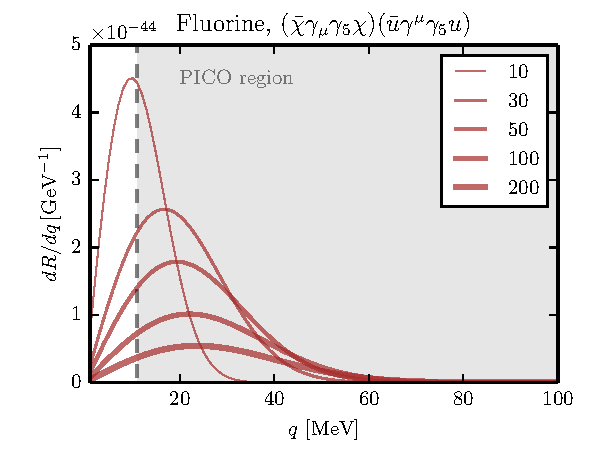
\includegraphics[scale=0.8]{figs/PlotqF19}\hspace*{0.2cm}
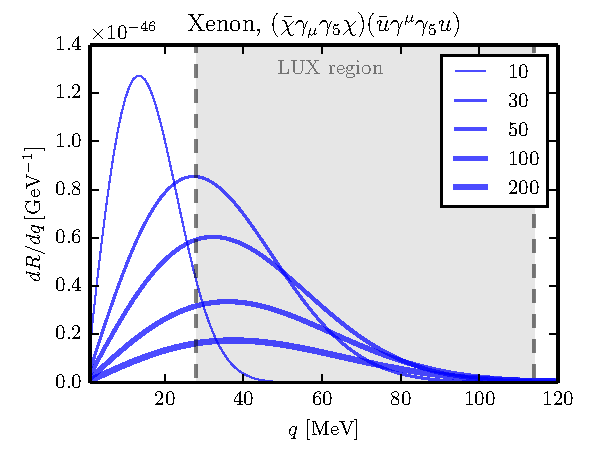
\includegraphics[scale=0.8]{figs/PlotqXe}
\end{center}
\caption[Momentum exchange distributions]{\em\label{fig:dRdq} The {\bfseries momentum exchange distributions}, $dR/dq$, for DM scattering rates on a representative light nucleus, ${}^{19}{\rm F}$ (left) and on heavy nucleus, {\rm Xe} (right), for spin-dependent scattering. The approximate experimental thresholds are denoted by dashed vertical lines. Figure from~\cite{Bishara:2017pfq}.   \label{fig:direct:qexchange}}
\end{figure}


In general, the energy transferred from DM to the nucleus as measured in the center of mass frame, is an ${\mathcal O}(1)$ fraction of the kinetic energy of the DM--nucleus two body system, 
$K=\mu_A v^2/2$, where  $\mu_A = M m_A/(M+m_A)$ is the reduced mass of the DM--nucleus system, and $v\approx 10^{-3}$ is the relative velocity.
Numerically,  $K\approx 20\keV$, if DM has a mass comparable to the heavy nuclei, $M\approx m_A\approx 100\GeV$.  
This is small enough that the scattering is elastic, i.e., that after collision the nucleus remains   in the same state  as before the collision. At the same time, $K$ is also large enough that the scattering event can be detected.

More precisely, a typical momentum exchange during the collision is $q\sim 20$ MeV for scattering on light nuclei, such as F, and $q\sim 60$ MeV for scattering on heavy nuclei, such as Xe (see 
fig.\fig{direct:qexchange}).
Experiments can tag the scattering events and reconstruct $K$ by observing
at least one of the following three end-products:
i) heat (phonons); ii) ionization; iii) scintillation. 






The expected number of events per unit of time, assuming that DM particles have velocity $v$, is given by
\beq
\hbox{event rate} = N_T \frac{\rho_{\odot}}{M} v \sigma_A \approx
\frac{1.5}{\hbox{yr}} \times \frac{m_T/A}{{\rm kg}}
\frac{\sigma_A}{10^{-39}\cm^2}\times 
\frac{\rho_{\odot}}{0.4\displaystyle\sfrac{\GeV}{\cm^3}}\times 
\frac{v}{200\displaystyle\sfrac{\km}{\rm s}}
\times \frac{100\GeV}{M},
\eeq
where $m_T = N_{T} m_{A} $ 
is the mass of the detector
composed of $N_{T}$ nuclei with atomic number $A$ and mass $m_{A}\approx A m_N$, where $m_N=0.939$~GeV is the nucleon mass, and $\sigma_A$ is the DM cross section for scattering on the {\em nucleus}. For comparison, a typical cross section for particles that interact via QCD such as $p, \pi$ is $\sigma \approx 10^{-26}\,\text{cm}^{2}$, while for neutrinos of energy $E_\nu$ scattering on nucleons, a scattering that is mediated by the weak force, the cross section is $\sigma_{\nu N\to \nu X}/E_\nu\approx 10^{-38}\,\text{cm}^2/\text{GeV}$. We see that for weak scale cross sections one can expect only a few events per kg of material per year. Note that the above  simple minded estimate has many caveats, which we will delve more into in the rest of this section. In particular, 
we assumed that the mean DM density in our local neighborhood is given by the value in eq.\eq{rhosun:value}. However, inhomogeneities are expected, and thus 
the solar system could be in an over- or under-density (probabilities are estimated by \arxivref{0801.3269}{Kamionkowski and Koushiappas} in~\cite{BoostFactorDD}), modifying the expected average scattering rates by orders of magnitude. 


The DM cross section for scattering on a {\em nucleus}, $\sigma_A$, is usually converted to a cross section for DM scattering on a {\em nucleon}, $\sigma_N$. 
Quite often such scattering does not depend on nuclear spin.
Then the main observable to be measured is the spin-independent cross section for DM scattering on nucleons,
$\sigma_N=\sigma_{\rm SI}$. This is related to the cross section for heavy DM scattering on nuclei as
$\sigma_{\rm SI}\approx \sigma_A/A^4$  
(see eq.~\eqref{eq:SI:param} below).

\begin{figure}[t]
\begin{center}
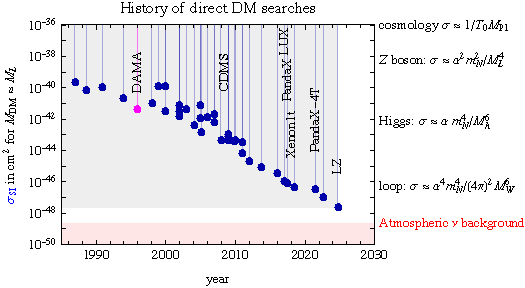
\includegraphics[width=0.8 \textwidth]{figs/directdetectionhistory} 
\end{center}
\caption[History of direct detection]{\em {\bfseries History of direct detection bounds} for spin-independent DM--nucleon scattering, setting the DM mass around the $Z$ boson mass. Only the most stringent bounds (blue) at any given moment are shown, along with the claimed DAMA signal (section~\ref{sec:DAMA}).}
\label{fig:history:direct}
\end{figure}


The historic progression of bounds on spin-independent scattering cross section is summarised in fig.\fig{history:direct}, 
assuming for concreteness DM with mass $M\approx M_Z$, which roughly maximises the bounds.
The most sensitive experiments at present, {\sc LZ} \cite{LZ}, {\sc Xenon1T} \cite{Xenon-1T} and {\sc PandaX-4T} \cite{PandaX-4T}, 
set a bound on the DM/nucleon cross section down to 
$ \sigma_{\rm SI}\circa{<}10^{-46}\cm^2$, with the complete $M$ dependence of the exclusion  shown in fig.\fig{sigmaSIbound}.
Figure\fig{history:direct}   also shows the expected  DM scattering cross sections for several examples of DM interactions:
\begin{itemize}
\item[$\triangleright$] DM particles which undergo strong interactions would have
$\sigma_{\rm SI} \sim 1/\Lambda_{\rm QCD}^2 \sim 10^{-26}\,{\rm cm}^2$.
As discussed in section~\ref{sec:SIMP}, such DM particles would have been stopped by collisions in the upper atmosphere and have been largely excluded.

\begin{figure}[t]
\begin{center}
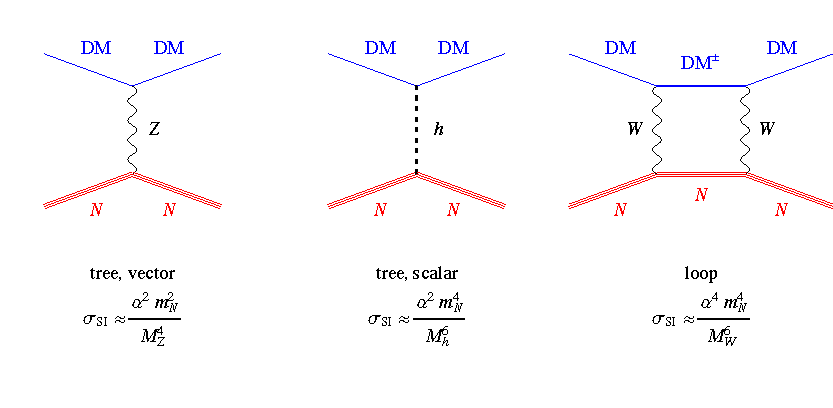
\includegraphics[width=0.8 \textwidth]{figs/DMsigmaSI} \vspace{-1.5cm}
\end{center}
\caption[Typical direct detection effects]{\em Typical values of the {\bfseries DM scattering} cross sections from tree level $Z$ exchange (left), Higgs exchange (middle), and 1 loop electroweak correction (right). 
}
\label{fig:direct:typical}
\end{figure}


\item[$\triangleright$] Tree-level $Z$ exchange would give 
$\sigma_{\rm SI} \sim  \alpha_{Y}^2 Y^2_{\rm DM} m_N^2/M_Z^4 \sim 10^{-38}\cm^2$ and is essentially excluded,
unless DM has a small (effective) hypercharge $|Y_{\rm DM}|  \circa{<} 10^{-4}$.

\item[$\triangleright$] Tree-level  Higgs exchange {(with one loop coupling to gluons)} would give $\sigma_{\rm SI} \sim \alpha_{\rm DM} m_N^4/M_h^6 \sim 10^{-43}\cm^2$
where $\alpha_{\rm DM} \sim y_{\rm DM}^2/4\pi$, if DM is a fermion with a Yukawa coupling
$y_{\rm DM}$, presently constrained to be smaller than about 0.1.


\item[$\triangleright$] DM with $\SU(2)_L$ interactions and $Y=0$ can 
scatter  through 1-loop electroweak diagrams as in fig.\fig{direct:typical},
giving $\sigma_{\rm SI} \sim \alpha_2^4 m_N^4/M_W^6 \sim 10^{-45}\cm^2$.
Computations find numerical factors of order $10^{-2}$
(see table~\ref{tab:MDM}), so this is allowed.
\end{itemize}
Experimental progress will become more difficult when experiments reach the background due to solar and atmospheric neutrinos, plotted as a grey region in  fig.\fig{sigmaSIbound} (bottom) and discussed further in section~\ref{nubck}.


\subsection{Direct detection of strongly-interacting DM}\label{sec:SIMP}
\index{Direct detection!of strongly-interacting DM}
In principle, DM particles could have large scattering cross sections with matter.\footnote{Usually, `strong interactions' is synonymous with `QCD interactions'. However, in the case of strongly interacting DM the large cross sections may be either due to QCD or due to new interactions. Note that `strongly interacting massive particle (SIMP)' acronym has been used both for the case where DM has strong interactions with normal matter, as well as for the case where there are strong interactions within the dark sector but only feeble interactions with normal matter.}
Such DM particles would hit the Earth with velocity $v \sim 10^{-3}$  (kinetic energy $E = M v^2 /2$)
and get stopped by the Earth's atmosphere, without reaching the underground detectors.
Heavy neutral particles loose energy in matter as~\cite{SIMP}
\beq\label{eq:dEdx}
\frac{d E}{d x} = -E \sum_A  n_A \sigma_A   \frac{2m_A }{M}   
=- 2 E \rho \langle A^4 \rangle \frac{ \sigma_{\rm SI}}{M}
\qquad \hbox{for $m_A\ll M$},
\eeq
where $n_A$ is the number density of nuclei with atomic number $A$ and mass $m_A \approx A m_N$, 
$2m_A/M$ is the fractional energy loss per collision, 
while $\sigma_A\approx \sigma_{\rm SI} \, A^2 (\sfrac{m_A}{m_N})^2$ is the coherently enhanced
cross section for DM scattering on a nucleus, with $\sigma_{\rm SI}$ denoting the spin independent scattering cross section for DM scattering on a single proton or neutron (assumed to be the same for simplicity, see also discussion in section \ref{sec:SI} below).
The number densities of targets in matter can be written as $n_A = f_A \rho/m_A$,  where
$\rho$ is the total mass density and $f_A$ the mass fraction of material $A$, such that $\sum_A f_A =1$.
Eq.\eq{dEdx} leads to the following expression for the energy loss of DM when passing through the material,
\beq
\label{eq:flightpathdEdx} E(x)=E_0  \exp\bigg[-
\frac{\TeV }{ M}
\frac{ \sigma_{\rm SI}}{\pi/\Lambda_{\rm QCD}^2}
\frac{\int \rho \,dx\,}{7\,{\rm kg}/{\rm m}^2}
\frac{\langle A^4 \rangle}{16.6^4}
 \bigg],
\eeq
where for convenience we normalized the $\sigma_{\rm SI}$ to the typical QCD cross section, $\pi/{\Lambda_{\rm QCD}^2}\approx 1.6 \cdot 10^{-26}\cm^2$.
The Earth's atmosphere has a column depth $\int \rho\, dx =10^4 \, {\rm kg/\m}^2$ and $\langle A^4 \rangle^{1/4} \approx 16.6$.
The crust  has $\langle A^4 \rangle^{1/4}\approx 31$ and density $\rho\approx 3\,{\rm g/cm}^3$.
This explains why underground detectors cannot probe too large values of $\sigma_{\rm SI}/M$, as plotted in fig.\fig{sigmaSIbound} (top).
Close to the upper boundary of the area excluded by the underground detectors (red shaded area in fig.\fig{sigmaSIbound} (top)), the strongly interacting DM particles undergo multiple interactions in detectors, a signature that is usually rejected in direct detection searches, and thus dedicated analyses of data are needed. This provides a {\em ceiling} to the reach of underground detectors, as pointed out by \arxivref{astro-ph/0301188}{Albuquerque and Baudis (2003)} and more recently refined by \arxivref{1712.04901}{Kavanagh (2018)}~\cite{SIMP}.

\smallskip

For larger cross sections, DM particles never reach the underground detectors.
These larger values of $\sigma_{\rm SI}$ can be tested by a combination of DM searches performed using surface detectors, airborne experiments on balloons, rockets or satellites~\cite{SIMP}. The extensive excluded areas are shaded in blue in fig.\fig{sigmaSIbound} (top). 
A related exclusion can be derived exploiting the fact that, upon multiple scatterings, heavy enough DM particles with galactic initial velocity $v \sim 10^{-3}$ slowly sink into the Earth, thermalizing with the atmosphere or the rock. Such a population of trapped, low-energy DM has been probed by  collisions on excited tantalum: its nucleus has
an excited state with angular momentum $\ell=9$, which is so long lived that its decay has never been observed. DM would de-excite the nucleus, which then places a bound $\sigma_{\rm SI}\lesssim 10^{-31}\cm^2$ at $M \sim\TeV$ (\arxivref{1911.07865}{Lehnert et al.~(2020)} in~\cite{SIMP}).

\smallskip

Another complementary exclusion (magenta region in fig.\fig{sigmaSIbound} (top)) arises from requiring that  the measured terrestrial heat flow is not appreciably altered by the energy deposited in annihilations of DM particles that got captured by the Earth (see \arxivref{0705.4298}{Mack et al.~(2007)}, \arxivref{1211.1951}{Mack \& Manohar~(2013)} and \arxivref{1909.11683}{Bramante et al.~(2020)}). 
\arxivref{2505.24070}{Cappiello and ~(2025)} extended this constrain down to about $\sigma_{\rm SI}\lesssim 10^{-38}\cm^2$ at $M \sim 80 \, \GeV$ by requiring that the inner core is not melted by dark matter annihilations. Note that these bounds therefore only apply to annihilating DM.

\smallskip

Very large cross sections (gray shaded area in fig.\fig{sigmaSIbound} (top)) are excluded by the absence of modifications in the CMB and the large scale structure power spectrum, since a large interaction between (cold) DM and baryonic matter would imply an excessive momentum transfer among the two species. This upper bound falls roughly at the same place as the constraints on DM self-interaction discussed in section \ref{sec:bullet}.
Slightly weaker constraints are obtained from the non-observation of a flux of $\gamma$-rays produced by the decay of neutral pions, which would have originated from collisions between the DM particles and the Galactic cosmic rays. BBN also imposes bounds, though orders of magnitude weaker than the ones above. All these bounds hold up to $M  \sim 10^{16}\GeV$, above which the DM flux becomes too small to be observable by the current DM detectors. 
A dedicated analysis using the massive {\sc Deap} detector reaches almost the Planck mass. 

\bigskip



Finally, the bounds discussed here apply to {\em spin-independent} (SI) DM/matter scattering (see section \ref{sec:SI}). A subset of analogous constraints for the {\em spin-dependent} (SD) scatterings (see section \ref{sec:SD}) have also been computed, though a systematic analysis is still lacking\footnote{The bounds from {\sc Icecube} on annihilating DM captured in the Sun (\arxivref{1001.1381}{Albuquerque and Perez de los Heros (2010)}~\cite{SIMP}) and from the heating of Jupiter (\arxivref{2309.02495}{Croon and Smirnov (2023)}~\cite{DMandplanets}) are relevant for the SD case. See also the discussion in section \ref{sec:DMinstars}.}. As a rule of thumb, the bounds on SD interactions derived from nuclear scatterings are about 3 to 5 orders of magnitude looser than the corresponding SI bounds, since the latter benefit from the $A^2$ scaling with the nuclear mass number $A$ (see section \ref{sec:SI}).
However, as pointed out by \arxivref{1907.10618}{Digman et al.~(2019)}, the constraints based on the scattering on {\em nuclei} at large values of the cross sections ($\sigma_{\rm SI} \gtrsim 10^{-32}- 10^{-27}$ cm$^2$) should be taken with care, as the $A^2$ scaling may fail.
The constraints based on the scattering on {\em protons}, such as those from the CMB and the cosmic rays, are not affected by these considerations.



 \begin{figure}[t]
$$
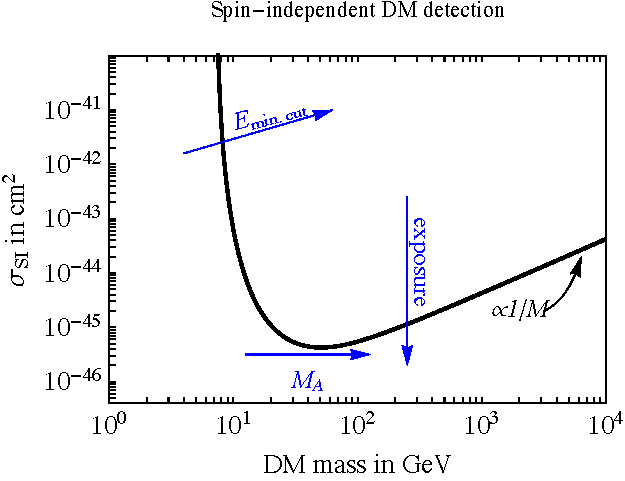
\includegraphics[width=0.47 \textwidth]{figs/directDDIlustrArrows}\qquad
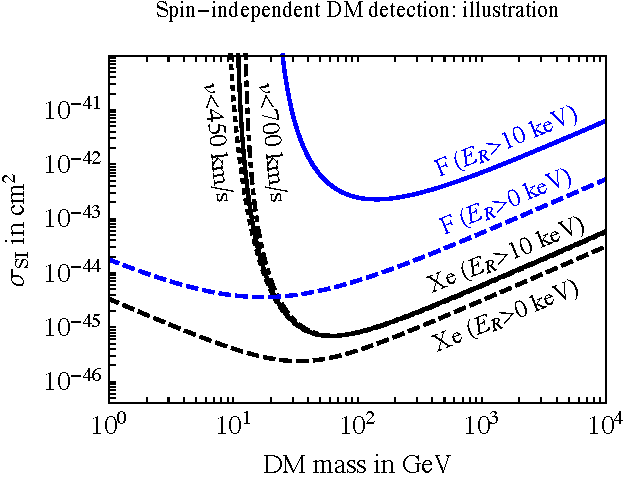
\includegraphics[width=0.47 \textwidth]{figs/directDDIlustr} 
$$
\caption[Direct detection bounds]{\em {\bfseries Left}: a {\bfseries typical exclusion curve} from a direct detection experiment, with cross sections and DM masses above the curve excluded. 
{\bfseries Right}: examples of exclusion curves for SI scattering on xenon (black curves) and fluorine (blue) for two choices of recoil energy cut, $E_R>10\,{\rm keV}$ (solid), and no energy cut (dashed), assuming no backgrounds. The variation on galactic escape velocity of the DM halo model, eq.~\eqref{eq:MB}, is only visible for low DM masses ($v_{\rm esc}=450 \,{\rm km/s}$, $550\,{\rm km/s}$, $700\, {\rm km/s}$ are shown  with dotted, solid and dot-dashed lines). }
\label{fig:DD:illustrations}
\end{figure}





\subsection{Direct detection of weakly-interacting DM: generalities}
\index{Direct detection!of weakly-interacting DM}
\label{SISD}

Next, we assume that DM particles interact weakly enough so that they reach the underground detectors.
The event rate of  DM scattering on nucleus, ${\rm DM}+{A}\to {\rm DM}+{A}$ (defined as\ the number of counts per time interval per target mass, $R_{\rm ev}=dN_e/dt\times 1/m_T$) is 
\beq
\label{eq:NevER}
\frac{dR_{\rm ev}}{dE_R}=\frac{N_{T}}{m_T}  \int_{v>v_{\rm min}}^\infty
\frac{d\sigma_A}{dE_R} v ~dn_{\rm DM}(\vec v), \qquad {\rm with }  \quad
d n_{\rm DM} = \frac{\rho_\oplus}{M} f_\oplus(\vec v) d^3 \vec v.
\eeq
Here $N_T$ is the number of nuclei in the target of mass $m_T$, and $E_R\sim {\mathcal O}({\rm keV})$ is the recoil energy of nucleus.  If there is more than one species of nuclei in the target, $N_T d\sigma_A/dE_R$ is replaced with a sum over different nuclei, $\sum_i N_{T,i}d\sigma_{A,i}/dE_R$. The integration is over the DM velocity in Earth's frame, $v$, with $\rho_\oplus$ the DM density at Earth's location. 
Normally this is the same as the DM density at the position of the solar system, 
$\rho_\oplus=\rho_\odot\approx 0.4 \GeV/{\rm cm}^{3}$, see eq.~\eqref{eq:rhosun:value}. The DM velocity distribution on Earth,  $f_\oplus(\vec v)$, is normalized such that $\int d^3 \vec v\, f_\oplus (v)=1$. It is obtained from the DM velocity distribution in the rest frame of the Galaxy  through a Galilean transformation to the Earth's frame, see eq.~\eqref{eq:fearth}.  For further details on the DM velocity distribution see section~\ref{sec:DMv}.



In order to transfer a kinetic energy $E_R$ to the nucleus, the incoming DM needs to have a minimal velocity
 \beq \label{eq:vmin}
 v_{\rm min} =
 \sqrt{\frac{m_{A} E_R}{2\mu_A^2}},\qquad \hbox{where}\qquad
 \mu_A= \frac{m_{A} M}{m_{A}+ M}\quad
 \hbox{is the nucleus--DM reduced mass.}
 \eeq
 The integral over the DM velocity in eq.~\eqref{eq:NevER} is then from $v_{\rm min}$ up to the escape velocity from the Galaxy (transformed into the Earth's frame), which is about $\sim 550 {\rm ~km}/{\rm sec}$, see eq.~\eqref{eq:vesc:range}. 
 Typical DM velocity is $\sim 200$ to $300  {\rm ~km}/{\rm sec}$, see eq.~\eqref{eq:rms:v0}.
 
 
 
In eq.~\eqref{eq:NevER} the particle physics is  encoded  in the DM--nucleus scattering cross section, $d\sigma_A/dE_R$. The description of this scattering is simplified by the fact that both the incoming DM and the nucleons inside the nucleus are non-relativistic, with typical velocities of ${\mathcal O}(10^{-3})$ and ${\mathcal O}(0.1)$, respectively. 
Ignoring velocity-suppressed terms there are only two possibilities for non-relativistic interactions: either the interactions involve nuclear spin, giving spin-dependent (SD) scattering, or they do not involve nuclear spin, resulting in spin-independent (SI) scattering.  
The UV models of dark matter more often than not lead to SI interactions.  If the SI interactions are present, these usually give the dominant contributions to the DM-nucleus scattering rates because of the coherent enhancement. The predictions for the SI scattering are also under better theoretical control, so that we focus on these first, 
followed by the discussion of  the SD scattering. The discussion of more general DM interactions, including velocity suppressed ones, is deferred  to section~\ref{sec:Effective:operators}. 


\subsection{Spin-independent scattering}\index{Direct detection!spin-independent}\index{Spin-independent scattering}
\label{sec:SI}
The SI cross section for DM scattering on {\em nucleus} is given by (see, e.g., G.\ Jungman et al.\ in \cite{otherpastDMreviews} or \cite{hep-ph/0010036,0912.4264,0803.2360})
\beq 
\label{eq:dsigmaAdER}
\frac{d\sigma_{{\rm SI}}^{A}}{dE_R} =\frac{m_A }{2v^2 \mu_N^2}
A^2  \sigma_{\rm SI} F^2(q),
\eeq
where $ \sigma_{\rm SI}$ is the average cross section for DM scattering on {\em nucleons} and $F(q)$ the nuclear form factor;  $A$ is the atomic mass number of the nucleus with charge $Z$;
$\mu_N$ is the reduced mass of the nucleon/DM system, $\mu_N=m_N M/(m_N+M)$ (for simplicity we work in the isospin limit, $m_p=m_n\equiv m_N$); 
the momentum exchange is given by $q = \sqrt{2m_A E_R}$ 
where $m_A \approx A m_N$ is the mass of the nucleus. The SI scattering rate of eq.~\eqref{eq:NevER} becomes
\beq
\frac{dR_{\rm ev}}{dE_R}= \frac{A^2  \sigma_{\rm SI} F^2(q)}{2 \mu_N^2}
 \frac{\rho_\oplus}{M} \eta(v_{\rm min}) , \qquad {\rm where} \quad \eta(v_{\rm min})= \int_{v>v_{\rm min}}^\infty
\frac{f_\oplus(\vec v)}{v}  d^3 \vec v,
\eeq
with $v_{\rm min}$ given in eq.~\eqref{eq:vmin}. Above, we assumed for simplicity that the target only contains a single species of nuclei. All the astrophysical uncertainties in predicting the DM scattering rates are contained in 
the local DM density $\rho_{\oplus}$ times a single function $\eta(v_{\rm min})$, encoding the dependence of the signal on the DM velocity distribution. 
These are then multiplied by the nuclear inputs such as the average cross section, $ \sigma_{\rm SI}$,  
given by\footnote{Note that  since $\sigma_{\rm SI}^{p(n)}\propto (c_1^{p(n)})^2$, it does not matter whether $\sigma_{\rm SI}^p$ or $\sigma_{\rm SI}^n$ is used on the r.h.s.\ of the first equality in eq.~\eqref{eq:hat:sigmaN}.}
\beq\label{eq:hat:sigmaN}
\sigma_{\rm SI}=\left(\frac{Z c_1^p+(A-Z) c_1^n}{A c_1^{p(n)}}\right)^2 \sigma_{\rm SI}^{p(n)}\approx \frac{1}{4}\sigma_{\rm SI}^{p}\pm\frac{1}{2}\sqrt{\sigma_{\rm SI}^{p}\sigma_{\rm SI}^{n}}+\frac{1}{4}\sigma_{\rm SI}^{n}, 
\eeq
where 
\beq
\sigma_{\rm SI}^{p(n)}=\frac{\mu_N^2}{\pi} (c_1^{p(n)})^2,
\eeq
is the SI cross section for  DM scattering on a single proton (neutron). Here, $c_1^p,c_1^n$ are the SI couplings of DM to non-relativistic protons and neutrons in the non-relativistic interaction Lagrangian (see also eq.~\eqref{eq:LNR} below),
\beq
\label{eq:SI:nonrel}
\Lag_{\rm int}^{\rm NR}= \sum_{N=n,p} c_1^N  1_N 1_{\rm DM},
\eeq
where $1_N$ ($1_{\rm DM}$) counts the number of nucleons (DM particles). The second, approximate, equality in \eqref{eq:hat:sigmaN} assumes $A\approx 2 Z$, which is a very good approximation for 
light nuclei, such as fluorine. The upper (lower) sign in eq.~\eqref{eq:hat:sigmaN} is for the same (opposite) signs of $c_1^p$ and $c_1^n$ (for simplicity we assume that these are real). For $c_1^p=-c_1^n$ one can therefore have an almost complete negative interference for the scattering on light nuclei. In heavier nuclei such as xenon or tungsten there are up to 50\% more neutrons than protons and thus the last relation in eq.~\eqref{eq:hat:sigmaN} becomes less accurate. 
In short, $ \sigma_{\rm SI}$ in eq.~\eqref{eq:hat:sigmaN} implicitly depends on the choice of target through $A$ and $Z$,
which means that cancellations between $c_1^p$ and $c_1^n$ cannot be exact for all isotopes and elements. 



The limit of small momenta exchanged between DM and nucleus, $q\to 0$, corresponds to the long wavelength limit or, equivalently, to the point particle approximation for the nucleus. In this limit DM couples coherently to all the nucleons inside the nucleus,  and so the scattering is coherently enhanced by a factor $A^2$. This is readily seen from eq.~\eqref{eq:dsigmaAdER} once the normalization of the nuclear form factor, $F(0)=1$, is taken into account. In the limit of small momenta transfers,  $q\to 0$, the  integrated cross section for DM scattering on nucleus is  
\beq
\label{eq:SI:param}
\sigma_{\rm SI}^A \Big|_{q\to0}= A^2  \sigma_{\rm SI}  \frac{\mu_{\chi A}^2}{\mu_{\chi N}^2}\approx  \sigma_{\rm SI}
\left\{
\begin{array}{ll}
A^2  & \text{for~} M\ll m_{N},
\\[1mm]
A^4/(1+ A m_N/M)^2 & \text{for~} m_{N}\ll M< m_{A},
\\[1mm]
A^4  &  \text{for~} M\gg m_{A},
\end{array}
\right.
\eeq
where the additional factor of $A^2$ in the scattering of heavy DM is due to the different
available recoil energies, 
\beq
\label{eq:ERmax}
E_{R,{\rm max}}=2\mu_{A(N)}^2 v^2/ m_{A(N)},
\eeq
 for scattering on nucleus (nucleon). For heavy DM, $M\gg m_{N,A}$,  we have $\mu_{\chi A}/\mu_{\chi N} \approx A$,  while $\mu_{\chi A}/\mu_{\chi N} \approx 1$ for GeV or sub-GeV DM, $M\ll m_{N,A}$.

\smallskip

 The decoherence for nonzero $q$ is reasonably well approximated by a Helm nuclear
form factor $F(q) = 3e^{-q^2 s^2/2}[\sin(qr)-qr\cos(qr)]/(qr)^3$, with $s=1$~fm, $r = \sqrt{R^2 - 5s^2}$, $R = 1.2A^{1/3}$~fm.
The decoherence can be important for typical momenta exchanges when scattering on heavy nuclei. For instance, $F(100{\rm~MeV})\big|_{A=19}=0.77$, $F(100{\rm~MeV})\big|_{A=132}=0.35$, for scattering on fluorine and xenon, respectively.  Note that eq.~\eqref{eq:dsigmaAdER}, where a single form factor  describes the nuclear response to both scattering on neutrons and on protons, applies only in the isospin limit. The isospin-breaking corrections are typically small, at the percent level. If they are included, the single $F$ is replaced by three form factors, one each for response to scattering on protons and on neutrons, and one for the interference term.\footnote{If the difference between proton and neutron distributions in the nucleus is taken into account,  eq.~\eqref{eq:dsigmaAdER} becomes,
\beq 
\frac{d\sigma_{{\rm SI}}^{A}}{dE_R} =\frac{m_A }{2 \pi v^2}
\Big[Z^2  \big( c_1^p F^{(p,p)}\big)^2+(A- Z)^2  \big( c_1^n F^{(n,n)}\big)^2 + 2 Z (A- Z)  c_1^n c_1^p \big(F^{(n,p)}\big)^2 \Big].
\eeq
In the isospin limit the three form factors are equal, and are the same as the one used in eq.~\eqref{eq:dsigmaAdER},  
$F^{(p,p)}=F^{(n,n)}=F^{(n,p)}=F$. 
In~\cite{Anand:2013yka} the definite isospin notation was used for the coupling coefficients, $c_i^{0(1)}=(c_i^p\pm c_i^n)/2$, along with squares of form factors of definite isospin,  i.e., the so-called nuclear response functions, $W_{M}^{00}, W_M^{01}, W_M^{11}$, where
$W_M^{00,11}=\kappa_A \big[Z^2 F^{(p,p)2}+ (A-Z)^2 F^{(n,n)2} \pm 2 Z(A-Z) F^{(n,p)2}\big] $ and $W_M^{01}= \kappa_A \big[Z^2 F^{(p,p)2}- (A-Z)^2 F^{(n,n)2}\big] $, with $\kappa_A= (2J_A+1)/4\pi $, and $J_A$ the spin of the nucleus. In the isospin limit, $W_M^{00}=\kappa_A A^2 F^2 $,  $W_M^{11}=\kappa_A (A-2Z)^2 F^2$, $W_M^{01}= - \kappa_A A(A-2Z) F^2 $, which shows that  in general $W_M^{00}\gg W_M^{01}, W_M^{11}$. In particular, for small $q$ we have, $W_M^{00}\simeq \kappa_A A^2$,  $W_M^{11}\simeq \kappa_A (A-2Z)^2 $, $W_M^{01}\simeq - \kappa_A A(A-2Z)$. Numerically, for fluorine $W_M^{00}\simeq 57$,  $W_M^{11}\simeq 0.16 $, $W_M^{01}\simeq - 3$, while for instance for heavy elements such as the xenon isotope ${}^{131}_{\,\,54}$Xe the SI form factors are significantly larger, $W_M^{00}\simeq 5.5 \cdot 10^3$,  $W_M^{11}\simeq 170 $, $W_M^{01}\simeq - 960$, as the result of coherent enhancement.
}

\medskip

An experimental bound on the number of scattering events, $N_{\rm ev}$, 
implies an upper bound on $\sigma_{\rm SI}$, see eq.s~\eqref{eq:NevER}, \eqref{eq:dsigmaAdER}. A typical bound in $M, \sigma_{\rm SI}$ plane is shown in fig.\fig{DD:illustrations} (left). The region above the curve is excluded. 
For large DM mass, $M\gg m_A$, the kinematics of the scattering is controlled by the mass of the nucleus, since this is the lighter of the two masses. This is the same as in the scattering of a bowling ball on a much lighter ping-pong ball ---  the momentum transfer is controlled by the relative velocity and by the mass of the ping pong ball only. In our expressions the DM mass enters through $v_{\rm min}$ dependence on $\mu_A$,  and through the DM number density, $n_{\rm DM}\propto 1/M$.  For heavy DM the reduced mass is approximately constant, $\mu_A \approx M_A$, so that
for heavy DM the direct detection bound on $\sigma_{\rm SI}$ scales as $\propto 1/M$. 

\smallskip

The exclusion in the low DM mass region is limited by the experimental
lower cut on the nuclear recoil energy, $E_R>E_{R\rm min}$.  
Experiments impose such a cut either due to the threshold in the sensitivity of the detectors or due to rising backgrounds at low recoil energies. 
Lowering $E_{R\rm min}$ makes experiments sensitive to lower DM masses, which is easy to understand from the kinematics. The lighter  the DM, the higher the minimal velocity for fixed $M_A$ and $E_R$. At some point, for lighter and lighter DM,  $v_{\rm min}$ becomes larger than the escape velocity in the Galaxy ($v_{\rm esc}\approx 550$ km/s), transformed to the Earth's frame, and the event rate goes to zero. Typical DM mass for which this happens in the present experiments is in the range of a few GeV. This is illustrated in the right panel of fig.\fig{DD:illustrations}. 
Without a cut on $E_R$ the experiments could in principle be sensitive to arbitrarily small DM masses (dashed curves). 
The sensitivity to  $\sigma_{\rm SI}$ is strongest for $M \approx M_A$, 
where the exact value 
depends on $E_{R\rm min}$ (compare the solid and dashed curves in the right panel of fig.\fig{DD:illustrations}). 

\medskip


Direct detection depends on relatively well-known DM astrophysical quantities: 
the DM density and the DM velocity distribution, $f_\oplus(\vec v)$. In fig.\fig{DD:illustrations} (right) we used the standard halo model with the escape velocity $v_{\rm esc}=550$ km/s. Variation in $v_{\rm esc}$ affects the exclusion for low DM masses, signalling that this probes the tails of the DM velocity distribution, especially for the scattering on heavy nuclei. 
This issue is discussed further in section~\ref{astrodirect}.

\bigskip

The current constraints on SI scattering cross section are shown in fig.~\ref{fig:sigmaSIbound}. The upper panel considers a wider set of cross sections and DM masses, as discussed in section \ref{sec:SIMP}. 
For smaller $\sigma_{\rm SI}$, the lower panel in  fig.~\ref{fig:sigmaSIbound} shows the current most stringent constraints from the underground detectors, using different materials. Note that direct detection experiments can exclude only DM cross sections that are small enough such that DM reaches the underground detectors (the upper boundary of the red excluded region in the upper panel in fig.~\ref{fig:sigmaSIbound}). For clarity we do not plot this upper boundary of exclusion for individual experiments in the lower panel in fig.~\ref{fig:sigmaSIbound}. For very large cross sections, above $\sigma_{\rm SI}\gtrsim 10^{33}\,\text{cm}^2$ it is also hard, if not next to impossible, to write down explicit models, where the mediators, because of their large couplings to visible matter, are not already completely excluded by other searches (such as the monojet searches at the LHC, rare kaon decays, cooling of stars, etc~\cite{2011.01939}). 


\begin{figure}[p]
\begin{center}
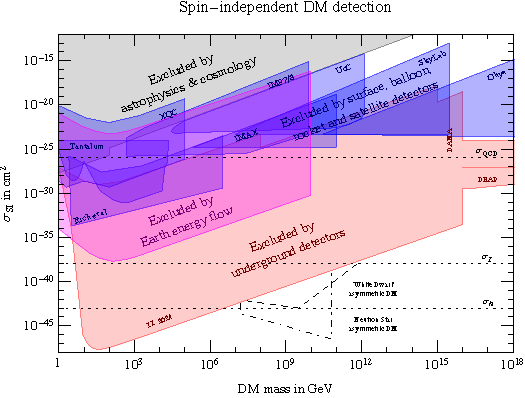
\includegraphics[width=0.72\textwidth]{figs/direct25Big} 
\\[2mm]
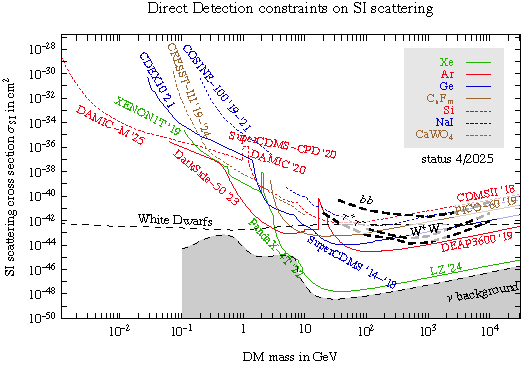
\includegraphics[width=0.72\textwidth]{figs/direct25} 
\end{center}
\vspace{-0.5cm}\caption[Bounds on $\sigma_{\rm SI}$]{\label{fig:sigmaSIbound}
\em {\bfseries Bounds on the spin-independent cross section} from Dark Matter direct detection. 
The {\bfseries top} panel shows a large range of cross sections, 
including the ranges for which DM does not reach the underground detectors, or leads to multiple scatterings 
(section~\ref{sec:SIMP} and~\cite{SIMP}).
The dashed (dot-dashed) black curves are bounds from White Dwarfs (Neutron Stars)
applicable to asymmetric DM (see sections \ref{sec:CaptureWD} and \ref{sec:CaptureNS}).
The dotted horizontal lines indicate the typical QCD, tree level $Z$, or $h$-mediated cross sections. 
This figure effectively connects with fig.\fig{MacroCompositeDM} at very large masses.
The {\bfseries bottom} panel shows the most stringent upper bounds, for different target materials, from the current underground detectors, table~\ref{tab:DDexp}, rescaled using the local DM density in eq.~\eqref{eq:rhosun:value}. For clarity we do not indicate the upper ranges of exclusions, where for $\sigma_{\rm SI}\sim 10^{-30}\cm^2$ the sub-$\GeV$ DM does not reach even the surface detectors (upper panel). For large DM masses the quoted exclusions are naively linearly extrapolated. The dashed black lines show the bounds that require annihilating DM:  from {\sc IceCube}~\cite{1612.05949} (for three DM annihilation modes that produce neutrinos in the Sun, 
see section~\ref{sec:DMnu}), and from White Dwarfs (see section \ref{sec:CaptureWD}). The neutrino background is discussed in section~\ref{nubck}.
The sub-$\GeV$ mass region is shown in further detail in fig.\fig{DirectDetectionSubGeVDM}.
}
\end{figure}



\subsection{Spin-dependent scattering}\index{Direct detection!spin-dependent}\index{Spin-dependent scattering}
\label{sec:SD}
If DM interactions with matter are predominantly through DM spin, $\vec S_{\rm DM}$, the description of the DM--nucleus scattering becomes more involved. In the non-relativistic limit there are  two types of interactions between DM spin $\vec S$ and the spin of nucleons, $\vec S_N$  (we use the notation of~\cite{Anand:2013yka,Bishara:2017pfq}), 
\beq
\label{eq:SD:nonrel}
\Lag_{\rm int}^{\rm NR}= \sum_{N=n,p} c_4^N \vec S\cdot \vec S_N+ c_6^N \Big(\vec S\cdot \frac{\vec q}{m_N}\Big)\Big( \vec S_N\cdot \frac{\vec q}{m_N}\Big),
\eeq
where $\vec q$ is the three-momentum transferred in the scattering.  Its size is $|\vec q|\sim \mu_A v\sim 100$ MeV for scattering on heavy nuclei, and $|\vec q|\sim \mu_N v\sim 1$ MeV for scattering on a free nucleon (in each case assuming $M \gtrsim m_{A,N}$).  The two non-relativistic coefficients, $c_4^N, c_6^N$, are affected differently by the QCD dynamics. 
For the case where heavy mediators couple DM to quarks, the $c_4^{p,n}$ coefficients do not depend on $q^2$  (the same as $c_1^{p,n}$ did not for the SI scattering). The $c_6^N(q^2)$, on the other hand, receive contributions from tree level exchanges of light mesons, $\pi^0$ and $\eta$, and are of parametric size $c_6^N\sim m_N^2/(m_\pi^2+\mb{q}^2)$, see eq.~\eqref{eq:c4N:c6N:axial} below. 

For DM scattering on free nucleons or on light nuclei the contributions from $c_6^N$ are suppressed by ${q}^2/m_\pi^2$ and it suffices to include only the $c_4^N$ terms in eq.~\eqref{eq:SD:nonrel}. This gives for the SD scattering of DM with incoming velocity $v$ on the unpolarized free nucleon:
\beq
\label{eq:SD:N}
\frac{d \sigma_{\rm SD}^N}{dE_R}= \frac{\sigma_{\rm SD}^N}{E_{R,{\rm max}}},\qquad \text{where}\qquad \sigma_{\rm SD}^N=J_{\rm DM}(J_{\rm DM}+1) \frac{(c_4^{N})^2\mu_N^2}{4\pi}
\eeq
is the total cross section, and $E_{R, {\rm max}}$ is the maximal recoil energy given in eq.~\eqref{eq:ERmax}, while $J_{\rm DM}$ is the DM spin. 

For SD scattering on heavy nuclei both terms in eq.~\eqref{eq:SD:nonrel} are of similar parametric size, giving the scattering cross section \cite{Anand:2013yka}\footnote{The other commonly used notation for the transverse spin form factors/nuclear response functions, 
see  e.g.~\cite{0803.2360,Bednyakov:2006ux}, is $S_{00(11)}(q)= W_{\Sigma'}^{00(11)}(q)/4$, $S_{01}(q)= W_{\Sigma'}^{01}(q)/2$. In the isospin limit the $S_{\tau\tau'}$ and $W_{\Sigma'}^{\tau\tau'}$ can be expressed in terms of the proton spin averaged over the  nucleus, $S_p$, and the averaged neutron spin, $S_n$. In terms of these, the $S_{\tau\tau'}$ nuclear form factors are given by $S_{00}=C(J_A) (S_p+S_n)^2$, $S_{11}=C(J_A)(S_p-S_n)^2$, $S_{01}=2 C(J_A) \big(S_p^2-S_n^2\big)$, where $C(J_A)=(2J_A+1)(J_A+1)/(4\pi J_A)$, with $J_A$ the spin of the nucleus. This then gives $W_{\Sigma'}^{00}=4  C(J_A) (S_p+S_n)^2$,   $W_{\Sigma'}^{11}=4 C(J_A) (S_p-S_n)^2$, $W_{\Sigma'}^{01}=4 C(J_A) (S_p^2-S_n^2)$. For nuclei with an unpaired proton, $S_p\simeq 0.5$, $S_n\simeq 0$ (and vice versa for nuclei with an unpaired neutron). An example of a nucleus with an unpaired proton is the stable isotope of fluorine ${}^{19}_{\,\,9}$F that has spin $J_A=1/2$,  
 so that $W_{\Sigma'}^{00}\simeq  W_{\Sigma'}^{11} \simeq W_{\Sigma'}^{01}\simeq 0.5$ in the long wavelength limit (a nuclear shell model calculation in \cite{Anand:2013yka} obtains $\approx 0.4$ for the three form factors). For the two stable xenon isotopes with nonzero nuclear spin, ${}^{129}_{\,\,54}$Xe with $J_A=1/2$ and ${}^{131}_{\,\,54}$Xe with $J_A=3/2$, one has both $S_p$ and $S_n$ nonzero and $W_{\rm \Sigma'}^{\tau\tau'}\sim {\mathcal O}(0.1)$.   }
\beq 
\label{eq:dsigmaAdER:SD}
\frac{d\sigma_{{\rm SD}}^{A}}{dE_R} =\frac{m_A }{6 v^2} \frac{J_{\rm DM} (J_{\rm DM}+1)}{2J_A+1} \sum_{\tau\tau'} \biggr[ c_4^\tau c_4^{\tau'} W_{\Sigma'}^{\tau\tau'}(q)+\biggr( \frac{ q^2}{m_N^2}\big(c_4^\tau c_6^{\tau'}+c_6^\tau c_4^{\tau'}\big)+\frac{ q^4}{m_N^2} c_6^\tau c_6^{\tau'} \biggr) W_{\Sigma''}^{\tau \tau'}(q)\biggr].
\eeq
The sum runs over isospin, $\tau,\tau'=0,1$, where the non-relativistic coefficients are $c_i^{0(1)}=(c_i^p\pm c_i^n)/2$. The nuclear response functions $W_{\Sigma'}^{\tau\tau'}(q^2), W_{\Sigma''}^{\tau \tau'}(q^2)$ give the transverse and the longitudinal responses to the DM spin interactions.  They take into account both the magnitude of the spin of the nucleus as well as the spatial distribution of the proton and neutron spins in the nucleus. In the nuclear shell model the SD nuclear form factors are expected to be larger, if the nucleus contains unpaired nucleons. Therefore the values of the SD form factors differ significantly between different isotopes of the same element.  In the long wavelength limit, $ q\to 0$, the two sets of nuclear response functions are proportional to each other, $W_{\Sigma'}^{\tau\tau'}(0)=2 W_{\Sigma''}^{\tau \tau'}(0)$,  but differ at finite $ q^2$. The values of the SD form factors are much more sensitive to the nuclear structure than the SI form factors are, and can differ substantially between different nuclear calculations (currently, the ab initio calculations are not possible for the heavy nuclei  and thus various approximations are required). Note however, that the suppression of SD form factors with increasing $q$ is slower than for the SI form factors. Typically, the SD nuclear response functions are suppressed by a factor of a few at $q=100$ MeV  and by about two orders of magnitude at $q=200$ MeV compared to their long wavelength values at $q=0$. 

\smallskip

If the $c_6^\tau$ contributions can be neglected, the SD scattering of DM on nucleus can be written in a form similar to the  SI scattering, eq.~\eqref{eq:hat:sigmaN},
\beq 
\label{eq:dsigmaAdER:SD:limit}
\frac{d\sigma_{{\rm SD}}^{A}}{dE_R} =\frac{m_A }{2v^2 \mu_N^2} \sigma_{\rm SD} S(q),
\eeq
where $\sigma_{\rm SD}=\sigma_{\rm SD}^p+\sigma_{\rm SD}^n$,
is the sum of cross sections for SD scattering on proton and neutron, eq.~\eqref{eq:SD:N}. The SD nuclear response functions are collected in
\beq
S(q)=\frac{1}{3(2J_A+1)}\Big[ W_{\Sigma'}^{00}+W_{\Sigma'}^{11}+2 c_{2\theta}W_{\Sigma'}^{01}+s_{2\theta}\big(W_{\Sigma'}^{00}-W_{\Sigma'}^{11}\big)\Big],
\eeq
where $c_{2\theta}\equiv\cos(2\theta)$ and $s_{2\theta}\equiv\sin(2\theta)$ parametrise the dependence on the ratio of SD couplings of DM to neutrons and protons, $\tan\theta\equiv c_4^n/c_4^p$. The simplified form of the cross section in eq.~\eqref{eq:dsigmaAdER:SD:limit} makes it easier to see that, unlike the SI cross section \eqref{eq:SI:param}, the SD scattering is not coherently enhanced. In the $ q\to 0$ limit the total SD scattering cross section is 
\beq
\sigma_{\rm SD}^A \Big|_{q\to0}= \sigma_{\rm SD} S(0)  \frac{\mu_{\chi A}^2}{\mu_{\chi N}^2}  \approx 
 \sigma_{\rm SD} S(0) \times
\left\{
\begin{matrix}
1& \text{for~} M\ll m_{N,A},
\\[1mm]
A^2  &  \text{for~} M\gg m_{N,A}.
\end{matrix}
\right.
\eeq
For GeV or sub-GeV DM the SD scattering cross section is given by SD scattering on individual nucleons, modified by the averaging over nuclear wave functions, encoded in $S(0)$. For heavy DM there is an extra $A^2$ factor due to the larger available kinetic energy.  Note that compared to the SI scattering, eq.~\eqref{eq:SI:param}, the SD cross section does not have  the additional enhancement due to the $A^2$ coherent factor.
This gives the weaker experimental bounds plotted in fig.\fig{DDSDbounds}.


Next, let us quantify how good is the approximation of neglecting the $\sigma_6^\tau$ terms in eq.~\eqref{eq:dsigmaAdER:SD}.
We illustrate this using two examples of DM interactions, the axial vector currents and the tensor interactions. For simplicity we assume that DM is a Dirac fermion, and that only couplings to $u$ and $d$ quarks are nonzero (a more complete treatment, including other possible interactions, is deferred to section~\ref{sec:Effective:operators}).





\subsubsection*{DM with axial-vector interaction} 
Here, we assume that the effective DM interaction, which follows from integrating out some heavy mediators, takes the form
(we use the notation and numerical values in \cite{Bishara:2017pfq})\footnote{For Majorana fermion DM, $\chi_{\rm M}$, the definition of the Wilson coefficient includes and extra factor of $1/2$ , $\Lag_{\rm int}=\sum_{q=u,d} \tfrac{1}{2} \hat {\cal C}_{4,q}^{(6)} \big(\bar \chi_{\rm M} \gamma^\mu \gamma_5 \chi_{\rm M})(\bar q \gamma_\mu \gamma_5 q)$. The factor of $1/2$ compensates the additional Wick contractions for the Majorana fermion, so that the expressions for the non-relativistic coefficients in \eqref{eq:c4N:c6N:axial} in terms of $\hat {\cal C}_{4,q}^{(6)}$ remain unchanged. } 
\beq
\Lag_{\rm int}=\sum_{q=u,d} \hat {\cal C}_{4,q}^{(6)} \big(\bar \chi \gamma^\mu \gamma_5 \chi)(\bar q \gamma_\mu \gamma_5 q),
\eeq
where the coefficients $\hat {\cal C}_{4,q}^{(6)}$ have dimensions of ${\rm mass}^{-2}$ and encode the particle physics --- the mass and the couplings of the heavy mediators (see also Section \ref{sec:benchmark:models} below). The two non-relativistic coefficients in eq.~\eqref{eq:SD:nonrel} are
\beq
\label{eq:c4N:c6N:axial}
c_4^N=- 4 \sum_{q=u,d}\Delta q_N \hat {\cal C}_{4,q}^{(6)}, \qquad c_6^N=\frac{m_N^2}{m_\pi^2+ q^2}\sum_{q=u,d} a_{P',\pi}^{q/N} \hat {\cal C}_{4,q}^{(6)},
\eeq
where $ \Delta u_p=\Delta d_n \equiv \Delta u=0.897(27)$ and $ \Delta d_p=\Delta u_n \equiv \Delta d=-0.376(27)$ are
the quark axial charges of proton and neutron (in the isospin limit), with $a_{P',\pi}^{u/p}=-a_{P',\pi}^{d/p}=a_{P',\pi}^{d/n}=-a_{P',\pi}^{u/n}=2(\Delta u-\Delta d)$. For weak scale DM, $M\sim {\mathcal O}(100\,{\rm GeV})$, the momentum exchange is comparable to the pion mass, $q\approx m_\pi$, see fig.~\ref{fig:direct:qexchange}. The two contributions in eq.~\eqref{eq:SD:nonrel} are thus parametrically similar in size, with the $c_6^N$ term only suppressed by $q^2/m_\pi^2$ (note that the $m_N^2$ factor in  \eqref{eq:c4N:c6N:axial} cancels the $1/m_N^2$ supression factor in eq.~\eqref{eq:SD:nonrel}).

\smallskip

We expect the $c_6^N$ terms to be numerically important for a heavy DM scattering on a heavy nucleus, such as xenon or tungsten. Ignoring $c_6^N$ term can then lead to an ${\mathcal O}(1)$ error in the predictions.\footnote{For instance, the predictions for the scattering rates for scattering of DM with mass $M=100\GeV$ on ${}^{131}$Xe 
are ${\mathcal O}(\{1\%, 30\%, 60\%, 20\%\})$ higher, if one ignores the $c_6^N$ terms, taking as the DM coupling benchmarks $\{\hat {\cal C}_{4,u}^{(6)}=\hat {\cal C}_{4,d}^{(6)},\hat {\cal C}_{4,u}^{(6)}=-\hat {\cal C}_{4,d}^{(6)}, \hat {\cal C}_{4,u}^{(6)}\ne 0, \hat {\cal C}_{4,d}^{(6)}\ne 0\}$ (keeping all the other couplings zero). Here, the $\hat {\cal C}_{4,u}^{(6)}=\hat {\cal C}_{4,d}^{(6)}$ benchmark is special, since in this case the pion pole contribution vanishes. The small correction comes from the exchange of the next lightest pseudoscalar meson, $\eta$.} 
In contrast, for the scattering of GeV/sub-GeV DM or for  the scattering on light nuclei, such as fluorine or oxygen, the $c_6^N$ terms can be safely ignored and one can use the simplified expression for the SD cross section, eq.~\eqref{eq:dsigmaAdER:SD:limit}.


\subsubsection*{DM with tensor interactions} 
If the DM interactions have the form
 \beq
 \label{eq:tensor:int}
\Lag_{\rm int}=\sum_{q=u,d} \hat {\cal C}_{9,q}^{(7)} m_q \big(\bar \chi \sigma^{\mu\nu} \chi)(\bar q \sigma_{\mu\nu} \gamma_5 q),
\eeq
the non-relativistic coefficients are 
\beq
\label{eq:c4:tensor}
c_4^N=8 \sum_{q=u,d}m_q A_{T,10}^{q/N}(0)  \hat {\cal C}_{9,q}^{(7)}, \qquad c_6^N=0,
\eeq
with the generalized tensor form factors at zero recoil given by the quark tensor charges, 
$A_{T,10}^{u/p(d/n)}(0)=g_T^u=0.794\pm0.0015$, $A_{T,10}^{d/p(u/n)}(0)=g_T^d=-0.204\pm0.08$.
The tensor interactions thus lead to pure $\vec S_{\rm DM}\cdot \vec S_N$ interactions. They are an example of DM couplings for which the simplified expression for the SD cross section, eq.~\eqref{eq:dsigmaAdER:SD:limit}, applies to both the scattering of GeV/sub-GeV and heavy DM, and for scattering on either light or heavy nuclei. 

\begin{figure}[p]
\begin{center}
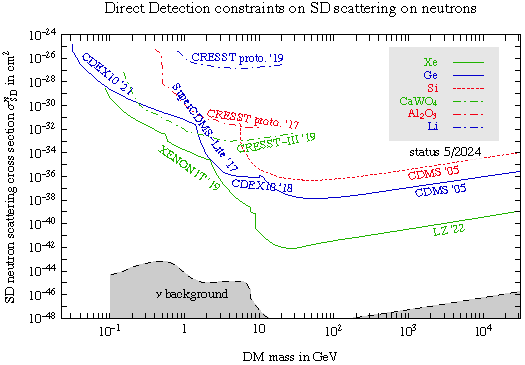
\includegraphics[width=0.72 \textwidth]{figs/Direct24SDn}
\\[2mm]
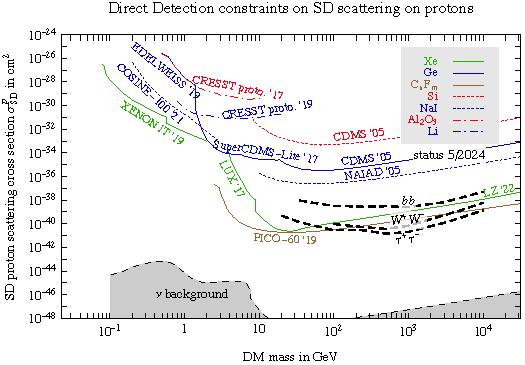
\includegraphics[width=0.72 \textwidth]{figs/Direct24SDp}
\end{center}
\caption[Bounds on $\sigma_{\rm SD}$]{\em\label{fig:DDSDbounds} 
As in fig.~\ref{fig:sigmaSIbound} (bottom), but for bounds on the {\bfseries spin-dependent} direct detection cross sections on neutrons 
$\sigma_{\rm SD}^n$ (top) and on protons
$\sigma_{\rm SD}^p$ (bottom) from underground detectors, 
and from {\sc IceCube}~\cite{1612.05949} 
(black dashed lines, for the indicated DM annihilation modes that produce neutrinos from the Sun,
as discussed in section~\ref{sec:DMnu}).}
\end{figure}





\subsection{Benchmark models for DM direct detection}
\label{sec:benchmark:models}
\index{Mediators!direct detection}

We list  benchmark models that lead to either SI or SD scattering, and the corresponding values  for the DM/nucleon scattering cross sections,  $\sSI^N$, $\sSD^N$.



\subsubsection*{$Z$-mediated DM interactions}\index{Mediators!$Z$}
The $Z$ boson might couple to DM so that the relevant part of the interaction Lagrangian is $\Lag_{\rm int}\supset - Z^\mu J_\mu$, where $J_\mu=J_\mu^{\rm SM}+ J_\mu^{\rm DM}$ is the sum of the SM and the DM current,
\beq\label{eq:DMZcouplings}
J_\mu = J_\mu^{\rm SM}+ \frac{g_2}{\cos\theta_{\rm W}} \left\{\begin{array}{ll}
\bar{\chi}\gamma_\mu (g^{V}_{\rm DM}+\gamma_5 g^{A}_{\rm DM})  \chi, & \hbox{if DM is a fermion $\chi$},\\
 g^S_{\rm DM}   [S^*( i\partial_\mu S)- (i\partial_\mu S^*) S], & \hbox{if DM is a scalar $S$,}
 \end{array}\right.
\eeq
with $g_2$ the weak coupling constant, and $\theta_W$ the weak mixing angle. 
The couplings $g^{V/A}_{\rm DM}$, $g^S_{\rm DM}$ depend on the details of the DM model. They are ${\mathcal O}(1)$ for DM that is part of an EW multiplet, and can be much less than one for DM mass eigenstates that are mostly EW singlet with only a small admixture of the EW charged component. 

Integrating out the $Z$ boson at tree level (see fig.\fig{direct:typical}a) gives the effective interaction between DM and the SM $\Lag_{\rm eff}=-J^{\rm SM} J^{\rm DM}/M_Z^2$. 
This leads to SI scattering if DM is either a fermion with vector interactions ($g_{\rm DM}^V \ne 0$), or if DM is a scalar. The non-relativistic coefficients of eq.\eq{SI:nonrel} are given by
\beq \label{eq:DDZmediated}
c_1^n = \Big(\frac{g_2}{2 c_{\rm W}}\Big)^2  \frac{g_{\rm DM}}{M_Z^2}\approx 0.13 \frac{g_{\rm DM}}{M_Z^2}, \qquad
c_1^p =\big(4s_{\rm W}^2-1\big)c_1^n \approx -0.01   \, \frac{g_{\rm DM}}{M_Z^2},
\eeq
where $c_W\equiv \cos\theta_W$, $s_W\equiv\sin\theta_W$.
Neglecting $|c_1^p|\ll |c_1^n|$ the SI scattering cross section is
\beq
\sigma_{\rm SI}\approx \frac{1}{4}\sigma_{\rm SI}^n =\frac{\GF^2 \mu_N^2}{2\pi} g_{\rm DM}^2
\approx 7.4 \,10^{-39}\cm^2 \,   \frac{\mu_N^2}{m_n^2}\,  g_{\rm DM}^2,
\eeq
where $g_{\rm DM}=g^V_{\rm DM} (g^S_{\rm DM})$ for fermion (scalar) DM. 
Large DM couplings, $g_{\rm DM}\sim {\mathcal O}(1)$, which one would obtain in the case of EW charged Dirac fermion DM, are excluded, see fig.\fig{history:direct}.
Direct detection data imply $g^{V,S}_{\rm DM} \circa{<} 2~10^{-4}$ for electroweak scale DM masses, $M\sim {\mathcal O}(M_Z)$, while the bound becomes progressively less stringent for heavier or lighter DM, see fig.~\ref{fig:sigmaSIbound}.

\medskip

Fermionic DM with just the axial couplings only produces spin-dependent scattering.
The vanishing of $g^{V}_{\rm DM}=0$ in eq.\eq{DMZcouplings}
is automatic for Majorana fermion DM, 
since for an anti-commuting Majorana fermions, $\bar \chi_i \gamma^\mu \chi_j=-\bar \chi_j \gamma^\mu \chi_i$, 
and thus Majorana fermion DM only has the axial coupling  $g^{A}_{\rm DM}$.
Integrating out the $Z$ gives 
\beq
\hat {\cal C}_{4,q}^{(6)}= \Big(\frac{g_2}{2 c_{\rm W}}\Big)^2 \frac{g_{\rm DM}^A}{M_Z^2}T_3^q, \qquad \text{where}\qquad T^u_d = \frac12, \quad T^d_3 = - \frac12,
\eeq
with the non-relativistic coefficients for SD scattering given in eq.\eq{c4N:c6N:axial}. This gives the same scattering cross section for DM scattering on protons and on neutrons, $\sigma_{\rm SD}^p=\sigma_{\rm SD}^n$, so that
\beq
\sigma_{\rm SD}=J_{\rm DM}(J_{\rm DM}+1) \frac{4 G_F^2 \mu_N^2}{\pi} \big(g_{\rm DM}^A\big)^2 \big(\Delta u-\Delta d\big)^2.
\eeq
The SD scattering is subject to a weaker direct detection bound, $\sigma_{\rm SD}\lesssim 10^{-41}\,\text{cm}^2$, cf. fig.\fig{DDSDbounds},
and thus $g_{\rm DM}^A \circa{<}10^{-2}$ for $M \sim M_Z$.

Small $g_{\rm DM}$ couplings can arise if DM has a small mixing with a hypothetical state that carries a hypercharge $Y\sim 1$. Another possibility is 
that DM has a large coupling to a hypothetical heavy  vector, $Z'$, and this has only a small mixing with the SM $Z$ boson. 
Integrating out the heavy $Z'$ gives an $\SU(2)_L$ gauge-invariant higher dimension effective interaction,  $\propto J_{\rm DM}^\mu  \big(H^\dagger D_\mu H\big)/M_{Z'}^2$, which after electroweak symmetry breaking gives a coupling between $Z$ and DM, $\Lag_{\rm int}\propto J_{\rm DM}^\mu Z_\mu v^2/M_{Z'}^2$.





\subsubsection*{Higgs-mediated DM interactions}\index{Mediators!Higgs}
The Higgs boson $h$ might couple to DM, $\Lag_{\rm int}\supset -h J_h$, where\footnote{We work after electroweak symmetry breaking. The $\SU(2)_L$-invariant generalization of the DM interaction to the Higgs is obtained by
promoting $h$ to $H^\dagger H/(\sqrt{2}v)$, see table~\ref{tab:SM}.} 
 \beq\label{eq:DMHiggscouplings}
J_h = J_h^{\rm SM}+  \left\{\begin{array}{ll}
\bar{\chi}(y_{\rm DM}+ i\gamma_5 \tilde y_{\rm DM})  \chi & \hbox{if DM is a fermion $\chi$,}
\\
 \lambda_{\rm DM}   v S^2/2 & \hbox{if DM is a real scalar $S$,}
 \\
 \lambda_{\rm DM}   v S^* S  & \hbox{if DM is a complex scalar $S$,}
 \end{array}\right.
 \eeq
with $v\approx 174\GeV$.
Integrating out the Higgs boson (see fig.\fig{direct:typical}b) gives  the effective interaction $\Lag_{\rm int}\supset J_h^{\rm SM} J_h^{\rm DM} /M_h^2$.
Scalar DM and fermionic DM with Yukawa interactions
produce the spin-independent scattering
with non-relativistic coefficients 
\beq 
\label{eq:c1n:c1p:Higgs}
c_1^n \simeq c_1^p =  \frac{f_N}{\sqrt 2} \frac{m_N }{M_h^2 v} 
\left\{\begin{array}{ll}
 y_{\rm DM}& \hbox{if DM is a Dirac fermion $\chi$},\\
 2 y_{\rm DM}& \hbox{if DM is a Majorana fermion $\chi$},\\
\lambda_{\rm DM} v/2 M & \hbox{if DM is a scalar $S$,}
 \end{array}\right. \eeq
 where $f_N\approx 0.3$ is the Higgs coupling to nucleons,\footnote{It is given by $f_N=2/9+\sum_{u,d,s} 7 \sigma_q^N/(9 m_N)$, where $\sigma_q^N$ is the scalar sigma term for quark $q$, $\sigma_q^N \bar u_N u_N=\langle N|m_q \bar q q|N\rangle$, and have the values $\sigma_s^N\approx 40$ MeV, and  $\sigma_{u,d}^N\approx 20-30$ MeV \cite{Bishara:2017pfq}.}  resulting in the SI cross section
\beq 
\label{eq:Higgs:sigmaSI}
\sigma_{\rm SI}=  \frac{\mu_N^2}{2 \pi} \Big(\frac{f_N m_N }{v}\Big)^2\frac{1}{M_h^4} 
\left\{\begin{array}{ll}
 y_{\rm DM}^2& \hbox{if DM is a Dirac fermion $\chi$},\\
 4 y_{\rm DM}^2& \hbox{if DM is a Majorana fermion $\chi$},\\
(\lambda_{\rm DM} v/2 M)^2 & \hbox{if DM is a scalar $S$.}
 \end{array}\right. \eeq
Compared to the SI scattering induced by the tree level exchange of $Z$, eq.\eq{DDZmediated},
the Higgs exchange induced scattering is suppressed by the Higgs couplings to matter, $f_N m_N /v$, and so
 the DM/Higgs couplings are less severely constrained.
Numerically, 
$y_{\rm DM}\lesssim 0.02$ for Dirac fermion DM with mass $M\sim {\mathcal O}(M_Z)$. Note that
$y_{\rm DM}\sim {\mathcal O}(1)$ has been excluded already for some time, see fig.\fig{history:direct}. 
For heavier DM the bound on $\sigma_{\rm SI}$ scales as $1/\sqrt{M}$, giving
 $y_{\rm DM}\lesssim 0.1 \sqrt{M/10\text{\,TeV}}$ for fermion DM, 
and  $\lambda_{\rm DM}\lesssim \big(M/2.0\text{\, TeV}\big)^{3/2}$ for scalar DM.
The pseudo-scalar Yukawa coupling, $\tilde y_{\rm DM}$, only gives spin-dependent scattering, which is further suppressed by the transferred momentum $q$, and is thus not subject to significant bounds.

\smallskip

The above cases for $\sigma_{\rm SI}$ in eq. \eqref{eq:Higgs:sigmaSI}
can be shortened into a single result by noticing that the Higgs contribution to the DM mass and the DM-Higgs coupling are related, given that they both arise from the same Higgs doublet field, $\langle H\rangle \to v+h/\sqrt 2$. Defining the Higgs-dependent DM mass $M(h) \gg m_N$, the tree level Higgs exchange induced direct-detection cross section is then for any DM spin given by,
\beq
\sigma_{\rm SI}=\frac{g_{\rm DM}^2}{2 \pi v^2} \frac{f_N^2 m_N^4 }{  M_h^4},\qquad\text{where}\quad
g_{\rm DM} = \frac{\partial M}{\partial h},
\eeq
and we approximated $\mu_N\simeq m_N$. 
For Dirac fermion DM, Majorana fermion DM, and scalar DM this reproduces the couplings in eq.\eq{c1n:c1p:Higgs}, $g_{\rm DM}=\{y_{\rm DM}, 2 y_{\rm DM}, \lambda_{\rm DM} v/2M\}$, respectively. 




\subsubsection*{$W$-mediated DM interactions}\index{Mediators!$W$}
DM might be the neutral component of a weak multiplet with hypercharge $Y=0$, in which case DM has a vanishing coupling to the $Z$ boson.
The scattering of DM on a nucleon is then induced at one loop by the weak couplings of DM to the $W^\pm$ gauge bosons, whereby the virtual emission of a $W^\pm$  changes DM to a charged component of the electroweak multiplet (see fig.\fig{direct:typical}c).
Integrating out the $W^\pm$ bosons 
gives a direct detection cross section 
\beq
 \sigma_{\rm SI} \sim \alpha^6 m_N^2/M_W^6 ,
\eeq
which is around or below the present experimental bounds, see fig.\fig{history:direct}.
Theories of this type are discussed in more detail in
section~\ref{sec:MDMDD}, see also fig.\fig{MDMOmega}a.



\subsubsection*{DM interactions mediated by a hypothetical dark photon} \index{Dark photon}
The interactions between DM and the SM can be mediated by light intermediate states. The difference with respect to the above results with the heavy mediators is that now even the $c_1^{N}$ in the non-relativistic Lagrangian \eqref{eq:SI:nonrel} are $q$ dependent, due to the propagator of the light mediator. An example of such a model is the dark photon, $A_\mu'$, a light vector boson that couples to the SM electromagnetic current, $J_{\rm em}^\mu$, and to DM, $\chi$, 
\beq
\Lag_{\rm int}\supset - e \epsilon J_{\rm em}^\mu A_\mu' - g_D A_\mu' \bar\chi \gamma^\mu \chi,
\eeq
where $\epsilon\ll1$ (see section \ref{sec:VectorPortal} for further details).
The non-relativistic coefficients in \eqref{eq:SI:nonrel} are given by
\beq\label{eq:c1p:c1n:darkphoton}
c_1^p=-\frac{e\varepsilon g_D}{q^2+m_{A'}^2}, \qquad c_1^n=0,
\eeq
so that for $m_{A'}$ lighter than a few 10s MeV the $c_1^p$ becomes $q^2$ dependent (see fig.~\ref{fig:direct:qexchange}). This means that the SI cross section for scattering on nuclei has additional $q$ dependence, 
\beq
\frac{d \sigma_{\rm SI}^A}{dE_R}=\frac{m_A}{2 \pi v^2} Z^2 \big[c_1^p (q)\big]^2,
\eeq
 and therefore the bounds on DM scattering derived from direct detection under the assumption of a constant $c_1^N$ need to be reexamined. The kinetic mixing parameter is constrained by other searches to be $10^{-3} \lesssim \epsilon \lesssim 10^{-5}$ for $m_{A'}\gtrsim 10$ MeV, see fig.~\ref{fig:dark:photon:constraints} below, while direct detection bounds require $\epsilon g_D\lesssim 10^{-10}$ for  DM with electroweak scale mass. For lighter DM masses the bounds from scattering on nuclei become less stringent. For sub-GeV DM, the main constraints on dark photon mediated scattering are obtained from bounds on possible DM scatterings on electrons, for which the dark photon model is one of the main benchmark models (see also the discussion in section~\ref{sec:direct:electrons}).




\begin{figure}[t]
\begin{center}
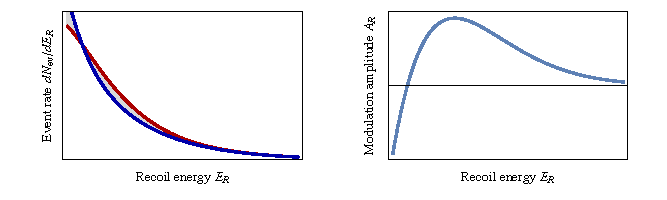
\includegraphics[width=0.9\textwidth]{figs/DDModAmpSchematic}
\end{center}
\caption[Direct detection modulation]{\em Illustrative example of {\bfseries DM-induced
nuclear recoil rates} $dN_{\rm ev}/dE_R$ at $t=$June 2nd (red) and $t=$Dec.\ 2nd (blue dashed).
The right handed plot shows the modulation amplitude $A_R(E_R)$.}
\label{fig:DD:modulation:DMwind}
\end{figure}


\subsection{Annual modulation}\label{DMmodulation}\index{Direct detection!annual modulation}\index{Annual modulation}
The direct detection event rate $dR_{\rm ev}/dE_R$, eq.~\eqref{eq:NevER}, contains an annual modulation induced by the Earth orbiting around the Sun \cite{DM:annual:mod}, see figure~\ref{fig:DD:modulation:DMwind}.
Indeed, as discussed in section~\ref{sec:DM:velocity:Earth},
the DM gas is on average at rest with respect to the galactic frame\footnote{The possibility that the DM halo co-rotates with the disk is addressed in section~\ref{sec:halocorotation}.},
where DM particles have an average velocity $v_0\approx {\mathcal O}(200)$km/s, see eq.~\eqref{eq:rms:v0}. 
The Sun orbits the center of the Galaxy and moves through the DM gas with a speed of about $v_\odot\approx233$~km/s, see eq.~\eqref{eq:vodot}. 
This induces a 233~km/s DM wind in the frame of the solar system. 
In addition, the Earth orbits the Sun with velocity $V_\oplus\approx 29.8\,{\rm km/s}$, 
which induces an annual modulation in the DM wind speed observed on Earth, see also fig.~\ref{fig:DMwind}. This affects the predicted DM scattering rate, $dR_{\rm ev}/dE_R$.  The integrand in~\eqref{eq:NevER} --- the DM flux, $v \, d n_{\rm DM}(\vec v)$ ---  changes slightly throughout the year, because the relative velocity between the Earth and the DM halo changes. Because the velocity integral  has a fixed lower cut-off at the minimal velocity $v_{\rm min}$, this induces a modulation in $dR_{\rm ev}/dE_R$, 
\beq
\label{eq:annual:mod}
\frac{dR_{\rm ev}}{dE_R}=\overline{\frac{dR_{\rm ev}}{dE_R}}\,
\Bigg[1+A_R(E_R) \cos\Big(\omega(t-t_c)\Big)\Bigg],
\eeq
where $\omega=2\pi/\yr$ and we expanded to first order in $V_\oplus$. 
The annual modulation amplitude is of order $A_R\approx {\mathcal O}(V_\oplus/v_{0,\odot})\approx 0.01-0.1$,
with the maximal rate expected on $t_c={\rm June~2}$, see eq.~\eqref{eq:voplus:time}. 
The average DM speed and thereby nuclear recoil energy is higher at $t_c$
than at $t_c + {\rm yr}/2 = $  December 2nd.
As a consequence, higher-energy events have a larger rate at $t_c$,
while lower-energy events have a larger rate at $t_c + {\rm yr}/2$.
If the velocity distribution $f_\oplus(\vec v)$ is known, the value of $E_R$ at which $A_R(E_R)$ changes sign can be used to measure the DM mass $M$.



\smallskip

There is also a day-night modulation induced by the rotation of Earth around its axis.  The {\bf diurnal modulation} is maximal for a detector on the equator, where the surface speed due to Earth's rotation is $\approx 0.5$ km/s. Even for this maximal case the diurnal modulation is still smaller than the annual modulation and can usually be neglected. A possible exception are the diurnal modulations of average scattering directions, which could be used as a signal in the future directional DM detectors, cf.~section~\ref{sec:dir:detection}. This is especially true for scattering of  sub-GeV DM, with masses below 100 MeV, where the diurnal modulation can be significantly enhanced by anisotropies in the target material such as organic crystals, which are planned to be used in the detection of such sub-GeV DM. Similarly, annual modulation can be important to distinguish signal from backgrounds also for sub-MeV dark matter scattering on electrons, which we discuss in section \ref{sec:direct:electrons}.




\subsection{Astrophysical uncertainties}
\label{astrodirect}
\index{DM abundance!direct detection}
\index{Direct detection!astrophysical uncertainties}
\index{Milky Way!direct detection}

The event rate for DM direct detection, eq.\eq{NevER},
depends on the product of the cross section times the local DM density, $\sigma_A \rho_\odot$,\footnote{Strictly speaking it depends on DM density on Earth, $\rho_\oplus$. In the vast majority of cases this is the same as the DM density at the position of the solar system, $\rho_\oplus=\rho_\odot$. However, there are known exceptions, see, e.g., \cite{MirrorDM:DD}.} 
and on the DM velocity distribution, $f_\oplus (\vec v)$, eq. \eqref{eq:fearth}. 
Converting a bound on $\rho_\odot \sigma_A$ into a bound on  $\sigma_A$ requires 
the determination of $\rho_\odot$ from astrophysical observations. 
While the local DM density has some uncertainty, see eq.~\eqref{eq:rhosun:value}, 
all the direct detection experiments assume a conventional value $\rho_\odot =0.3$~GeV/cm${}^3$ when interpreting their results, about $30\%$ less than the present best value of $0.4$~GeV/cm${}^3$ 
quoted in eq.~\eqref{eq:rhosun:value} and used throughout this review. 
The commonly used value of $\rho_\odot$ facilitates a quick comparison between different experiments. 
A different $\rho_\odot$ implies a rescaling of all bounds on $\sigma_A$, as we did for the bounds shown in fig.s \ref{fig:sigmaSIbound}, \ref{fig:DDSDbounds}, and \ref{fig:DDSIelec:bounds}.

The dependence of bounds on the local DM velocity distribution, $f_{\oplus}(\vec v)= f(\vec v+\vec v_\oplus(t))$, is less trivial. The astrophysical uncertainties in $f(\vec v)$ can sometimes lead to large uncertainties. 
This is especially true for the $\sigma_{\rm SI, SD}(M)$ exclusion curves at low DM masses, controlled by the $E_{R\rm min}$ threshold, see fig.~\ref{fig:DD:illustrations}.   
In this parameter region the  scatterings come from DM with velocities close to the Galactic escape velocity. 
For such velocities a large galactic variance of $f(\vec v)$ is expected, as shown by the $N$ body simulations, see fig.~\ref{fig:vel:dep}. This translates to a significant uncertainty in the expected event rates in direct detection and complicates the comparison of direct detection bounds obtained using different nuclei.
For simplicity this issue is often ignored and the bounds on DM scattering are plotted using the standard DM halo model, eq.~\eqref{eq:MB}.

\smallskip


If the dependence on $f_{\oplus}$ is important for the problem at hand, one can scan over a collection of reasonable  DM velocity distributions, such as discussed in section~\ref{sec:DMv}.
One can be even more conservative, however, and compare the results of direct detection experiments 
in a way that is independent of astrophysical uncertainties (`halo independent method'). The crucial insight is that the recoil energy $E_R$ is directly related to $v_{\rm min}$, see eq.~\eqref{eq:vmin}. The distribution of events, $d R_{\rm ev}/dE_R$, can thus be translated into the $v_{\rm min}$ space. In the $v_{\rm min}$ space the properly normalised $d R_{\rm ev}/dE_R$ distributions from all experiments should look the same. 

For instance, for SI scattering, where $d\sigma_A^{\rm SI}/dE_R\propto 1/v^2$, 
eq.~\eqref{eq:dsigmaAdER}, one can rewrite the scattering rate, eq.~\eqref{eq:NevER}, as~\cite{Astro:out}
\beq\label{eq:astro:indep}
\frac{d R_{\rm ev}}{dE_R}=\tilde  \eta(v_{\rm min}) \frac{dH_A}{dE_R} ,
\eeq
where the velocity dependence is encoded entirely in the function
\beq
\tilde \eta(v_{\rm min})=\frac{\rho_\oplus \sigma_\text{ref}}{M}\int_{v_{\rm min}}^\infty d^3 \vec v\, \frac{f_\oplus(\vec v)}{v},
\eeq
where $v_{\rm min}$ is given in eq. \eqref{eq:vmin}.
Here, $\sigma_\text{ref}$ is a reference cross section, for which we take the average total cross section for DM scattering on a single proton and a single neutron, $\sigma_\text{ref}=(\sigma_p^{\rm SI} +\sigma _n^{\rm SI})/2$ (other choices are equally viable). The remaining  factor in eq.~\eqref{eq:astro:indep} does not depend on DM velocity profile at all
\beq
\frac{dH_A}{dE_R}= \frac{N_T}{m_T}  v^2 \frac{d\sigma_A^{\rm SI}}{dE_R}=\frac{m_A}{2m_T\mu_N^2}\frac{ \sigma_{\rm SI}}{\sigma_\text{ref}}A^2 F^2(q).
\eeq
In the last equality we used eq.~\eqref{eq:dsigmaAdER}. The function $dH_A/dE_R$ differs for different nuclei, because of changes in $m_A$, $\sigma_{\rm SI}$, $A$, and $F(q)$.
On the other hand, the normalized scattering rate $\frac{d R_{\rm ev}}{dE_R}/\frac{dH_A}{dE_R}$ is the same for all nuclei, when expressed as a function of $v_{\rm min}$.
 Particle physics is encoded in $\sigma_{\rm SI}$ and $\sigma_{\rm ref}$, where $\sigma_{\rm SI}$ depends on the choice of the nuclear target, while $\sigma_{\rm ref}$ by definition does not. The ratio $\sigma_{\rm SI}/\sigma_\text{ref}$ only depends on the ratio of DM couplings to protons and neutrons, $c_1^p/c_1^n$. Choosing this ratio, and fixing the DM mass $M$, completely determines $dH_A/dE_R$ for each nuclear target.  Barring cancellations one has $ \sigma_{\rm SI}/\sigma_\text{ref}\sim {\mathcal O}(1)$, and thus the dependence of $dH_A/dE_R$ on the assumed particle physics is relatively mild. Furthermore, for not too light DM, $M\gg m_N$, the reduced mass $\mu_N\simeq m_N$ is almost completely independent of the value of $M$, and so is $dH_A/dE_R$.  

\smallskip

Fixing the DM mass $M$ and `particle physics', i.e., the ratio $c_1^p/c_1^n$,  
the experimental bound on ${d R_{\rm ev}}/{dE_R}$ 
implies a bound on $\tilde  \eta(v_{\rm min})$, where $v_{\rm min}=(E_R m_A/2)^{1/2}/\mu_A$ is determined by the measured recoil energy, $E_R$. A nonzero  signal, ${d R_{\rm ev}}/{dE_R}$,  would similarly imply a measurement of $\tilde  \eta(v_{\rm min})$. One can thus map all the bounds on (or measurements of) the scattering rates, ${d R_{\rm ev}}/{dE_R}$,  into the exclusion lines (signal regions) in the $(v_{\rm min},\tilde \eta)$ plane. If a signal from one experiment, translated to a nonzero value of $\tilde \eta (v_{\rm min})$, is contradicted by a bound from another experiment, then the potential DM SI scattering signal is excluded irrespective of the DM velocity profile. Note that in this comparison  the DM mass and particle physics couplings needed to be held fixed. To completely exclude the putative DM scattering signal one needs to marginalize over different values of $M$, and different ratios of particle physics couplings, $c_1^p/c_1^n$. 
The outlined statistical procedure is aided by the fact that $\tilde \eta(v_{\rm min})$ is a monotonically decreasing function.
The approach has been extended to include annual modulation, as well as general DM couplings  to nucleons~\cite{Astro:out}.




\subsection{Effective operators}\label{sec:Effective:operators}
\index{Direct detection!effective operators}
\index{Effective operators!direct detection}

If the interactions between dark and SM particles
are mediated by particles heavier than the typical momentum exchange in direct detection, $q\lesssim 200$ MeV, 
it is convenient to integrate out the heavy mediators and end up with an Effective Field Theory (EFT) description of the interactions with DM (just like the electro-weak theory is approximated at low energies by Fermi four-fermion effective operators).
As a simple example consider a scalar mediator, $\phi$,  that couples to both the DM $\chi$ and quarks, 
with the interaction Lagrangian $\Lag\supset y_\chi \,\phi \bar\chi \chi+ y_q\, \phi \bar q q$. 
The resulting DM/quark scattering amplitude ${\cal M}$ is given by
\begin{equation}
i{\cal M}=- i  \big(\bar u_\chi u_\chi\big)\frac{y_\chi y_q}{q_\mu q^\mu-m_\phi^2} \big(\bar u_q u_q\big) \stackrel{q\ll m_\phi}{\simeq}
 i \frac{ y_\chi y_q}{m_\phi^2} \big(\bar u_\chi u_\chi\big) \big(\bar u_q u_q\big) 
 +{\mathcal O}\Big(\frac{q^2}{m_\phi^2}\Big),
\end{equation}
where we expanded in $q^2/m_\phi^2 \ll 1$ and kept the leading term only. 
DM scattering is then equally well described by the 
local interaction operator  
${\cal C} \big(\bar \chi \chi\big)\big(\bar q q\big)$, 
where  all the relevant physics of the mediator is encoded in the value of its coefficient, ${\cal C}=y_\chi y_q/m_\phi^2$.
This EFT approach to direct detection is illustrated in fig.~\ref{fig:scalar:matching}. 
It allows to be quite agnostic about the high-energy theory of DM:
the only thing that matters for direct detection is the effective interaction.

\begin{figure}[!t]
\begin{center}
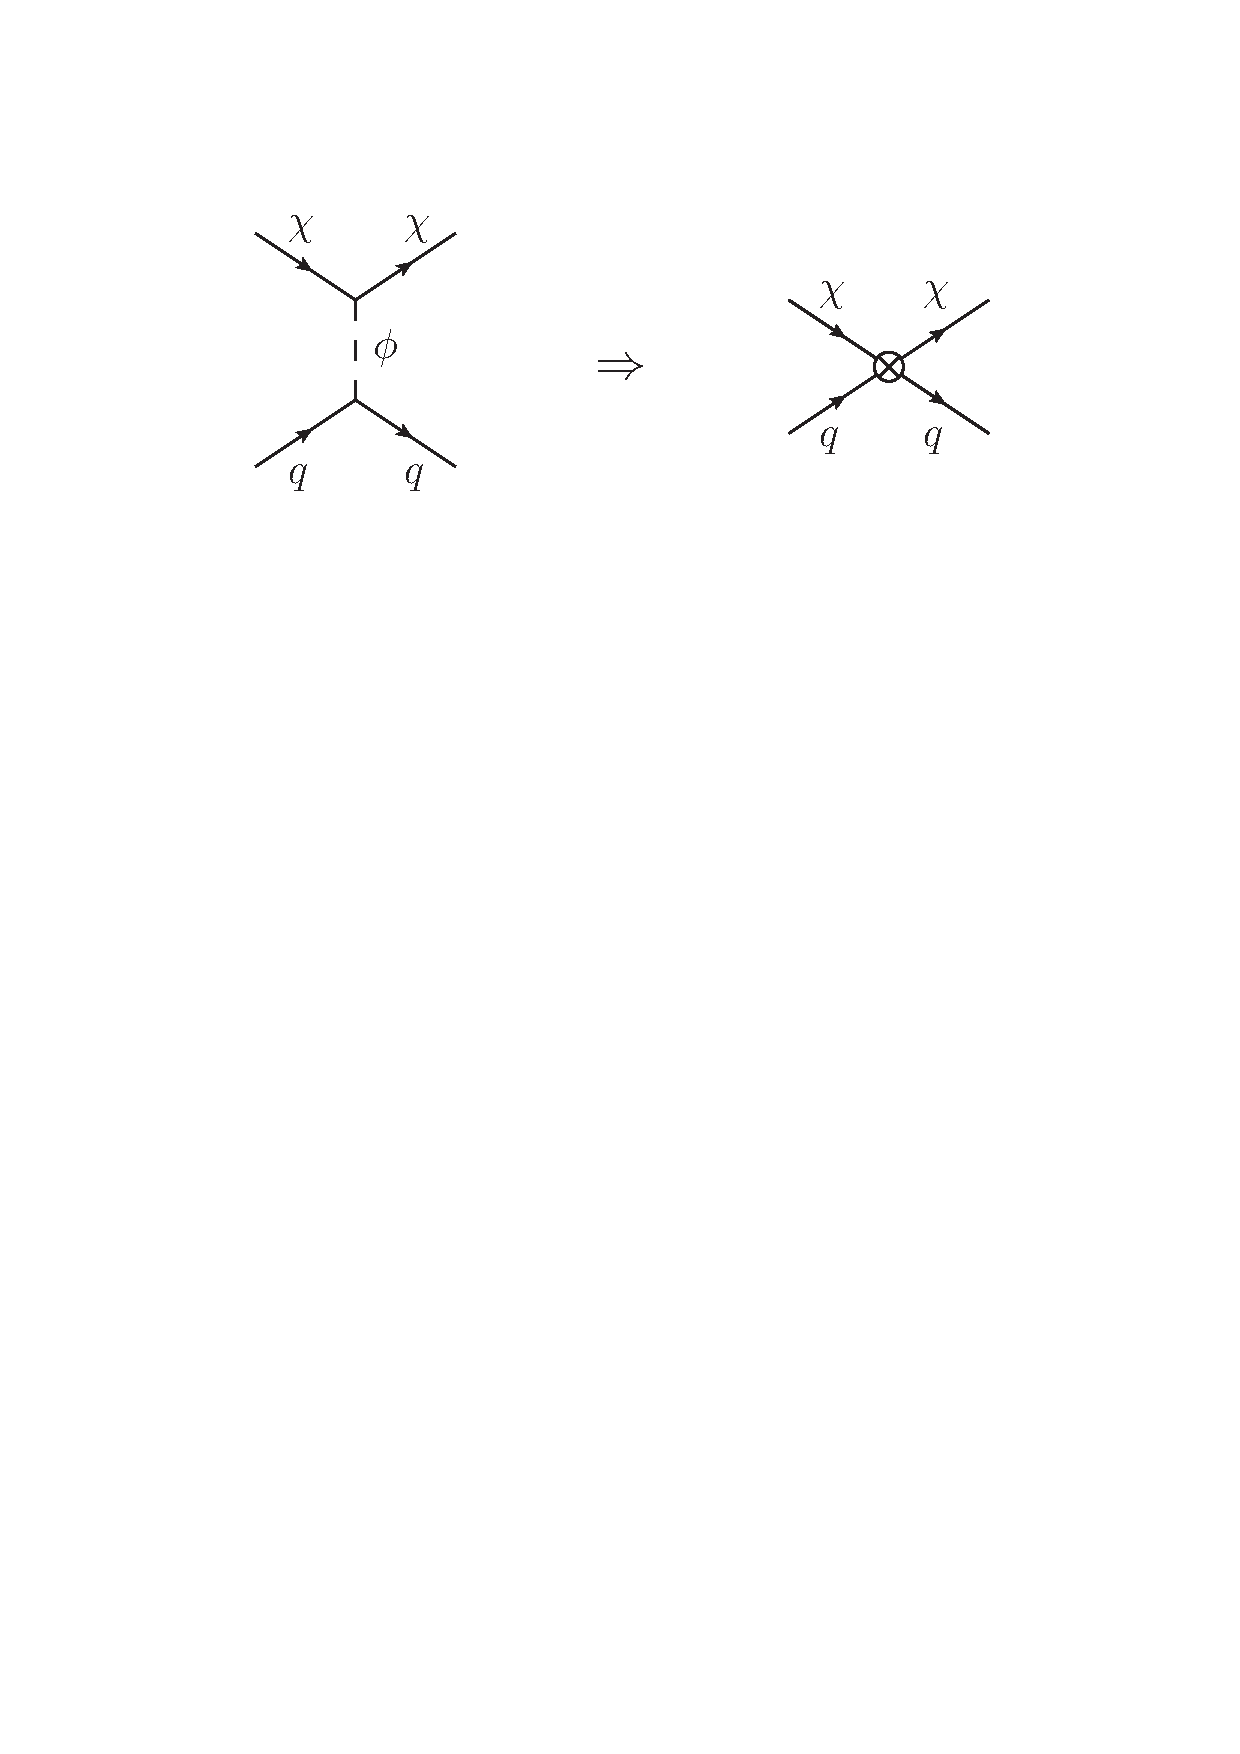
\includegraphics[scale=0.7]{figs/scalar_matching.pdf}
\end{center}
\caption[Direct detection EFT example]{\label{fig:scalar:matching}\em Sample model where DM interacts with the SM 
via a scalar mediator $\phi$ that couples to quarks.}
\end{figure}
 
Effective operators are conveniently ordered in terms of their dimensionality,
\begin{equation}\label{eq:lightDM:Lnf5}
\Lag_{\rm EFT}=\sum_{a,d}
\frac{{\cal C}_{a}^{(d)}}{\Lambda^{d-4}}  \Op_a^{(d)}. 
\end{equation}
Here the ${\cal C}_{a}^{(d)}$ are dimensionless coefficients encoding the UV couplings, while the scale
$\Lambda$ can be identified with the mass of the mediators  (in the above example $\Lambda=m_\phi$). 
The sums run over
dimensions of the operators, $d=\{5,6,7,\ldots\}$, and 
labels $a$, denoting operators with differing field contents and Lorentz structures.
Operators with lowest dimensions typically dominate the scattering rate,
so that stopping at $d=7$ provides a quite general and accurate approximation.


\begin{figure}[t]\centering
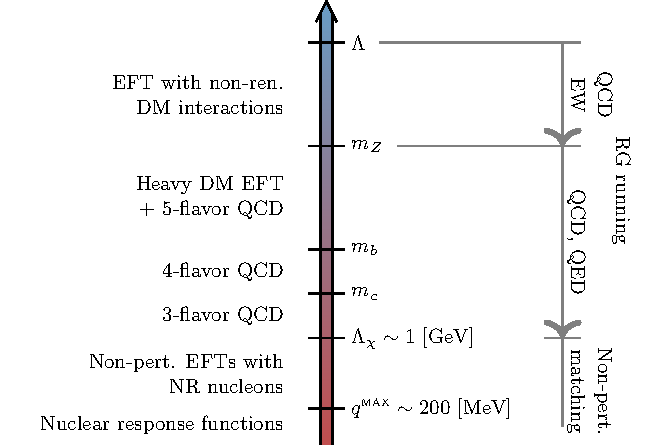
\includegraphics[scale=1]{figs/tower-of-efts}
\caption[EFT for direct detection]{\label{fig:eft-tower}\em 
The tower of effective field theories linking the UV scale $\Lambda$ to the scale
  of interactions between the nucleons and the DM. (From~\cite{Bishara:2018vix}.)}
\end{figure}

\smallskip

The EFT description of DM interactions has the following two main uses.
First, it allows to relate the results of different direct detection experiments with minimal assumptions about the origin of DM interactions. For instance, if a single direct detection experiment observes a putative signal of DM, while all  the other experiments only set limits, the immediate question would be: 
do the other experiments exclude such a DM signal? 
Using DM EFTs, one can answer such a question for all the models of DM for which the mediators are heavier than a few 100 MeV, such that a few coefficients ${\cal C}_{a}^{(d)}$ in eq.~\eqref{eq:lightDM:Lnf5}
describe all experiments.

Second, DM EFTs can be used to relate the processes involving DM that occur at very different energies, $\mu$. 
Concerning collider signals,
the typical energy for DM production at the LHC  (to be discussed in section~\ref{sec:EFTs?})
is set by the cuts on the visible final state particles and is typically around a TeV.
Concerning indirect detection signals,
annihilations of two non-relativistic DM particles release energy $2M$ into
SM particles, so that the appropriate EFT that describes such indirect detection signals
includes all particles lighter than DM.
The structure of the EFT describing DM interactions depends on the typical energy (or momentum) exchange, the scale $\mu$. 
Instead of a single DM EFT there is a tower of different DM EFTs, depending on the scale $\mu$, as illustrated in fig.~\ref{fig:eft-tower} for heavy mediators and electroweak scale DM mass (i.e.~$\Lambda\gg v_{\rm EW}\sim M$). 


At a particular scale $\mu$ the appropriate EFT includes the relevant propagating degrees of freedom. 
At the highest energy $\mu\sim \Lambda$ one needs the
full theory of DM interactions.
At $\mu\lesssim \Lambda$ the mediators can be integrated out, leading to an EFT
with non-renormalizable interactions between the DM and SM particles.
At $\mu\lesssim M_Z$ the top quark, the Higgs, and the $W,Z$ bosons can be integrated out
and the DM interactions are therefore
described by non-renormalizable operators in an EFT that contains only
DM and the light SM particles: the photon, the gluons, the leptons, the $b$, $c$, $s$, $d$, $u$ quarks.
At $\mu\sim m_b$ one integrates out the bottom quark, 
and at $\mu \sim m_c$ the charm quark. 
Finally, at
$\mu\sim {\mathcal O}(1)$~GeV a non-perturbative matching to a
chiral EFT with pions and nucleons is performed. 
This is then used to obtain the hadronic matrix elements for DM scattering on nuclei. 
Furthermore, DM can be conveniently described by a non-relativistic field at energies below its mass.

\smallskip
  
Quantum corrections can be important and need to be taken into account
when obtaining the low-energy EFT from the high-scale physics at $\mu\sim \Lambda$.
Fig.~\ref{fig:RG:EFT} illustrates three such examples of radiative corrections. 
For instance (left panel), if DM couples to the Higgs, integrating out the Higgs and the top quark at $\mu\simeq v_{\rm EW}$  induces  an effective coupling of DM to gluons. 
Even though this contribution is loop suppressed, it can be numerically important  for direct detection scattering since nucleons have a large gluon content.
Another example are the one loop exchanges of weak bosons, since these distinguish between left-handed and right-handed SM fields. Such radiative corrections can induce DM couplings to vector SM  currents, even if in the UV theory the DM particle couples only to the axial SM currents (at tree level). 
Axial and vector currents have very different non-relativistic limits, and thus the induced mixing of operators can be numerically important. Finally, even if DM couples only to leptons at tree level, the radiative corrections such as the photon exchange in the right panel in fig.~\ref{fig:RG:EFT}  
induce DM couplings to quarks, and thus scattering of DM on nuclei. 

In the rest of this section we focus on the DM EFT appropriate around the QCD scale  $\mu\sim 2\GeV$ 
and how such interactions of DM with quarks, gluons and photons induce scattering on nuclei. 
That is, we are interested in the last three steps in fig.~\ref{fig:eft-tower}: 3-flavor QCD, non-perturbative EFT with non-relativistic nucleons, and the nuclear response functions. 

\begin{figure}[!t]
\begin{center}
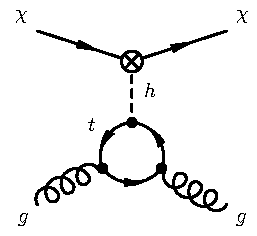
\includegraphics[scale=0.8]{figs/dim7-gg.pdf}~~~~
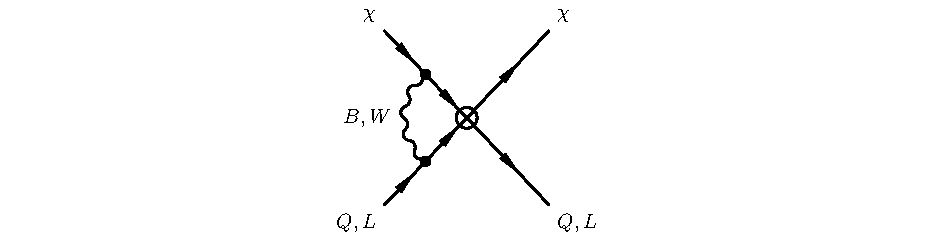
\includegraphics[scale=0.8]{figs/D6_4ferm.pdf}~~~~
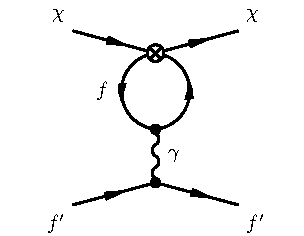
\includegraphics[scale=0.8]{figs/d6-photon-penguin.pdf}
\end{center}
\caption[DM EFT]{\label{fig:RG:EFT}\em Examples of one loop corrections that induce couplings to gluons (left), mix operators with different non-relativistic limits (middle), mix leptophilic and leptophobic interactions (right).  
(From \cite{Bishara:2018vix}.)}

\end{figure}

\subsubsection*{Quark level DM effective field theory}\index{Effective operators!quark level}  
We first focus on the DM EFT with three quark flavors, which has as propagating degrees of freedom the light quarks, $u,d,s$, the gluons, photons, and SM leptons. For definiteness we set $\mu=2\GeV$, which is a conventional scale choice for lattice QCD determinations of the nuclear matrix elements. 
The form of the operators in the EFT Lagrangian in eq.~\eqref{eq:lightDM:Lnf5} depends on whether DM is a scalar, a fermion or some higher spin particle. 
For instance, the complete basis for the EFT expansion up to dimension 7 contains 8 operators of dimension 6 for complex scalar DM. 
For a Dirac fermion DM there are two operators of dimension 5, four operators of dimension 6 and twenty-two operators of dimension 7, not counting fermion flavor multiplicities~\cite{Brod:2017bsw}. 

\smallskip

To gain  further insight we focus on DM as a spin 1/2 Dirac fermion $\chi$, 
and write the subset of operators, which are phenomenologically  most interesting.  
\begin{enumerate}
\item[5)] The two dimension-five operators  are (in the notation of~\cite{Brod:2017bsw})
\begin{equation}
\label{eq:dim5:nf5:Q1Q2:light}
\Op_{1}^{(5)} = \frac{e}{8 \pi^2} (\bar \chi \sigma^{\mu\nu}\chi)
 F_{\mu\nu} \,, \qquad \Op_2^{(5)} = \frac{e }{8 \pi^2} (\bar
\chi \sigma^{\mu\nu} i\gamma_5 \chi) F_{\mu\nu} \,,
\end{equation}
where $F_{\mu\nu}=\partial_\mu A_\nu-\partial_\nu A_\mu$ is the electromagnetic field strength tensor.  
The magnetic dipole operator $\Op_1^{(5)}$ is CP-even, while the electric
dipole operator $\Op_2^{(5)}$ is CP-odd. 
Both flip DM chirality.
Due to gauge invariance these operators are generated 
by integrating out heavy mediators at loop level \cite{DM:EM:moments},
and thereby include a loop suppression factor $e/8\pi^2$.


\item[6)] The dimension-six operators are
\begin{align}
\Op_{1,q}^{(6)} & = (\bar \chi \gamma_\mu \chi) (\bar q \gamma^\mu q),
 &\Op_{2,q}^{(6)} &= (\bar \chi\gamma_\mu\gamma_5 \chi)(\bar q \gamma^\mu q), \label{eq:dim6EW:Q1Q2:light}
  \\ 
\Op_{3,q}^{(6)} & = (\bar \chi \gamma_\mu \chi)(\bar q \gamma^\mu \gamma_5 q)\,,
  & \Op_{4,q}^{(6)}& = (\bar
\chi\gamma_\mu\gamma_5 \chi)(\bar q \gamma^\mu \gamma_5 q).\label{eq:dim6EW:Q3Q4:light}
\end{align}
Here, $q=\{u,d,s\}$ denote the light quarks (we limit ourselves
to flavor-conserving operators).  Such dimension 6 operators are for instance generated by $Z$-mediated DM interactions discussed in  section~\ref{sec:benchmark:models}. 
While tree level $Z$ exchange generates all four types of coefficients, ${\cal C}_{i,q}^{(6)}$, the phenomenologically relevant ones are ${\cal C}_{1,q}^{(6)}$, since these induce SI scattering.\footnote{Identifying $\Lambda=m_Z$ as the mass of the mediator gives  ${\cal C}_{1,q}^{(6)}=g_{\rm DM}\big(T^3_q-2 s_W^2 Q_q\big)/2$, where $T^3_q=1/2$ is the weak isospin of $u$ quark and $T^3_q=-1/2$ for $d,s$ quarks, and $Q_q$ the electromagnetic charge of quark $q$.} The other operators give SD scattering and can thus be neglected, if ${\cal C}_{i,q}^{(6)}$ is nonzero. The situation is different for Majorana fermion DM for which the  $\Op_{1,q}^{(6)}$ and $\Op_{3,q}^{(6)}$ operators vanish, and thus SD scattering is the leading interaction.\footnote{For Majorana DM the definitions of the operators conventionally include an extra factor of $1/2$ in the four component notation, to compensate for the two possible contractions, simplifying the common notation for cross sections. See \cite{Bishara:2017nnn} for more details.} 

\item[7)] A selection of (possibly phenomenologically most interesting) dimension-seven operators is
\allowdisplaybreaks
\begin{align}
\Op_{1}^{(7)} & = \frac{\alpha_{\rm s}}{12\pi} (\bar \chi \chi)
 G^{a\mu\nu}G_{\mu\nu}^a\,, 
& \Op_{4}^{(7)}& = \frac{\alpha_{\rm s}}{8\pi}
(\bar \chi i \gamma_5 \chi) G^{a\mu\nu}\widetilde G_{\mu\nu}^a \,, \label{eq:dim7:Q3Q4:light}
\\
\Op_{5,q}^{(7)} & = m_q (\bar \chi \chi)( \bar q q)\,, 
&
\Op_{9,q}^{(7)} & = m_q (\bar \chi \sigma^{\mu\nu} \chi) (\bar q \sigma_{\mu\nu} q)\,, 
 \label{eq:dim7EW:Q9Q10:light} 
\\
\label{eq:Q7:11}
\Op^{(7)}_{11} &= \frac{\alpha}{12\pi}(\bar{\chi}\chi)\,
F^{\mu\nu} F_{\mu\nu}\,,  &\quad
\Op^{(7)}_{14} &=  \frac{\alpha}{8\pi}(\bar{\chi}i\gamma_5\chi)\, F^{\mu\nu} \tilde{F}_{\mu\nu}\,,
\end{align}
where the labeling is as in~\cite{Brod:2017bsw}, where also the remaining dimension 7 operators can be found.
Here, $G_{\mu\nu}^a$ is the QCD field strength tensor, and
$\widetilde G_{\mu\nu} = \frac{1}{2}\varepsilon_{\mu\nu\rho\sigma}
G^{\rho\sigma}$ is its dual, and similarly for the electromagnetic 
field strength tensor $F_{\mu\nu}$ and its dual $\tilde F_{\mu\nu}$. 
The index $a=\{1,\dots,8\}$ runs over color $\SU(3)_c$ generators. 
\end{enumerate}
Dimension seven operators are encountered as the leading operators in many theories of DM. 
For instance, the Higgs-mediated DM interactions ($y_{\rm DM}\ne0$ in eq.~\eqref{eq:DMHiggscouplings}) generate the operator $\Op_{1}^{(7)}$ 
at one loop after the Higgs and $t, b,c$ quarks are integrated out, see the left panel in fig.~\ref{fig:RG:EFT}. 
The operators $\Op_{5,q}^{(7)}$ arise from tree level Higgs exchanges, with the corresponding coefficients given by 
${\cal C}_{1}^{(7)}/\Lambda^3 =- 3{\cal C}_{5,q}^{(7)}/\Lambda^3= 3 y_{\rm DM} /(\sqrt 2 v M_h^2 )$.  
For this result, note that the proportionality of Higgs/quarks couplings to quark masses was already included in the definition of the $\Op_{5,q}^{(7)}$ operators. Furthermore, the dependence on the heavy quark mass drops out in the result for the gluonic operator due to the required two chiral insertions in the loop cancelling the $1/m_q^2$ suppression from the loop propagators. The operators $\Op_{1}^{(7)}$ and $\Op_{5,q}^{(7)}$ all lead to SI scattering. 

\smallskip

Pseudo-scalar mediators such as Goldstone bosons and axion-like (ALP) particles,
on the other hand, couple to pseudo-scalar SM currents. Integrating out the ALP mediators coupling to gluons or photons
generates the operators $\Op_{4}^{(7)}$ and $\Op_{14}^{(7)}$, respectively. If ALP couples to quarks, it would also generate the equivalent of $\Op_{5,q}^{(7)}$ but with $i\gamma_5$ insertions in the scalar currents. All these operators lead to SD scattering.\index{Axion-like particles}

\smallskip

The Rayleigh operators $\Op^{(7)}_{11}, \Op^{(7)}_{14}$, encode DM polarizability, which can be a sign of composite nature of DM or of (pseudo-)scalar mediators coupling to photons.  Rayleigh operators are not the  operators of lowest dimension that involve the DM and electromagnetic fields, because these arise already at dimension 5, see $\Op^{(5)}_{1,2}$ in eq.~\eqref{eq:dim5:nf5:Q1Q2:light}. 
However, these magnetic and electric dipole moment operators  vanish for Majorana fermion DM, 
so it may well be that the interactions to the SM only arise from DM polarizability, i.e., from the operators such as $\Op^{(7)}_{11}, \Op^{(7)}_{14}$. 
In fact, this would be a generic feature of models  where DM is a Majorana fermion, that is not coupled to colored particles~\cite{DM:Rayleigh}. 

\medskip

Eq.s \eqref{eq:dim5:nf5:Q1Q2:light} to \eqref{eq:Q7:11} (plus the undisplayed dimension 7 operators) 
provide a complete basis of EFT operators of up to and including dimension 7.
One could have chosen a different basis, with a different set of operators. 
Different choices of EFT bases describe the same physics: using equations of motion and performing integration per parts, 
one can convert these to the basis used here.
For example, our basis
does not include the DM anapole operator, $(\bar \chi\gamma_5\gamma^\mu\chi) \partial^\nu F_{\mu\nu}$, which is sometimes assumed to give dominant interactions for DM with higher dimension electromagnetic interactions (the so called {\em anapole DM}~\cite{Anapole:DM}).\index{Anapole} 
The electromagnetic equations of motion
$\partial^\mu F_{\mu\nu}+\sum_f e Q_f \bar f\gamma_\nu f=0$ allow to express the anapole operator in terms of the dimension 6 operators in eq.~\eqref{eq:dim6EW:Q1Q2:light} and \eqref{eq:dim6EW:Q3Q4:light},
\beq
\bar \chi\gamma_5\gamma^\mu\chi \partial^\nu F_{\mu\nu}= -  \sum_{q=u,d,s} e Q_q\Op_{2,q}^{(6)}-   \sum_{\ell=e,\mu,\tau} eQ_\ell\Op_{2,\ell}^{(6)}.
\eeq

\smallskip

The EFT operators depend on DM spin.  The EFT contains a smaller number of operators, if DM is a scalar $S$. 
We again list those relevant for the EFT at $\mu=2$ GeV:  the  effective interactions  only start at
dimension six, with the full operator basis given by 
\begin{align}
\label{eq:dim6:Q1Q2:light:scalar}
\Op_{1,f}^{(6)} & = \big(S^* i\overset{\leftrightarrow}{\partial_\mu} S\big) (\bar f \gamma^\mu f)\,,
 &\Op_{2,f}^{(6)} &= \big(S^* i\overset{\leftrightarrow}{\partial_\mu} S\big)(\bar f \gamma^\mu \gamma_5 f)\,, 
 \\
 \label{eq:dim6:Q3Q4:light:scalar}
 \Op_{3,f}^{(6)} & = m_f (S^* S)( \bar f f)\,, 
&{\cal
  Q}_{4,f}^{(6)} &= m_f (S^* S)( \bar f i\gamma_5 f)\,,
\\
\label{eq:dim6:Q5Q6:light:scalar}
  \Op_5^{(6)} & = \frac{\alpha_{\rm s}}{12\pi} (S^* S)
 G^{a\mu\nu}G_{\mu\nu}^a\,, 
 & \Op_6^{(6)} &= \frac{\alpha_{\rm s}}{8\pi} (S^* S) G^{a\mu\nu}\widetilde G_{\mu\nu}^a\,,
\\
  \label{eq:dim6:Q7Q8:light:scalar} 
 \Op_{7}^{(6)} &=\frac{\alpha}{\pi}(S^*
S) F^{\mu\nu}F_{\mu\nu}\,, 
& \Op_{8}^{(6)} &=\frac{3\alpha}{\pi}(S^*
S) F^{\mu\nu} \tilde F_{\mu\nu}\,, &~&
\end{align}
where $S^*\overset{\leftrightarrow}{\partial_\mu}S  \equiv  S^* (\partial_\mu S)- (\partial_\mu S^*)
S$. The operators $\Op_4^{(6)}$, $\Op_6^{(6)}$, and $\Op_8^{(6)}$ are CP-odd, while all the others are CP-even. 
The above operators for scalar DM have a similar form to a subset of the effective operators for spin 1/2 DM. 
The vector and axial vector currents operators  are of dimension 6 both for scalar DM, eq.~\eqref{eq:dim6:Q1Q2:light:scalar}, and for fermion DM, eq.s~\eqref{eq:dim6EW:Q1Q2:light}, \eqref{eq:dim6EW:Q3Q4:light}. 
The scalar operators in eq.s~\eqref{eq:dim6:Q3Q4:light:scalar} to \eqref{eq:dim6:Q5Q6:light:scalar} 
correspond to the dimension 7 scalar operator $\Op_{5,q}^{(7)}$ for fermion DM in eq.~\eqref{eq:dim6EW:Q1Q2:light}, along with the undisplayed operators with extra $i\gamma_5$ insertions.
In each case there are less operators for scalar DM, because for fermionic DM one can insert $\gamma_5$ in the currents and thus have scalar and pseudo-scalar (or vector and axial-vector) currents on the DM side. 
In the non-relativistic limit such operators give as the leading effect the coupling to the DM spin for spin $1/2$ DM, which is then absent for spin 0 DM.

Another important consequence of scalar DM being spin 0 is that the spin $1/2$ DM can have a nonzero magnetic or electric moment, i.e., it is possible to write down the dimension 5 operators in eq.~\eqref{eq:dim5:nf5:Q1Q2:light}. There is nothing equivalent for scalar DM. For uncharged DM the first nonzero electromagnetic interaction are therefore dimension 6 polarizability operators, eq.~\eqref{eq:dim6:Q7Q8:light:scalar}.


 

\medskip

\subsubsection*{Heavy DM effective theory}
\index{Effective operators!heavy DM}  

The above DM EFT holds if DM is much lighter than the mediators, $M\ll \Lambda$. 
If this is not the case, the expansion in powers of $1/\Lambda$ becomes problematic: since $(M/\Lambda)^n$ is no longer small, higher and higher dimension operators give sizeable contributions. 
As a concrete example consider two operators: a dimension 6 vector-vector operator and a dimension 8 operator with extra derivatives acting on DM,
\beq
\label{eq:example:HDMET}
\frac{1}{\Lambda^2} (\bar \chi \gamma_\mu \chi) (\bar q \gamma^\mu q)\sim \frac{M v_0^\mu}{\Lambda^2} (\bar \chi \chi) (\bar q \gamma^\mu q), \qquad \frac{1}{\Lambda^4} (\bar \chi \gamma_\mu \partial^2 \chi) (\bar q \gamma^\mu q)\sim \frac{M^3 v_0^\mu}{\Lambda^4} (\bar \chi \chi) (\bar q \gamma^\mu q).
\eeq
Above, we wrote the DM four-momentum as $p_\chi^\mu=M v_0^\mu +k^\mu$,
where $M v_0^\mu$ with $v_0^\mu=(1,0,0,0)$ is the four-momentum of DM at rest in the laboratory frame,
and $k^\mu\sim {\mathcal O}(M v)\ll M$ is  the remaining small momentum due to the relative motion of DM, with velocity $v \sim 10^{-3}$. In writing the r.h.s.~expressions in eq.~\eqref{eq:example:HDMET} we neglected corrections suppressed by powers of $k/M$. 
Eq.~\eqref{eq:example:HDMET} shows that, after taking the non-relativistic DM wave functions,
operators with dimension 6 and 8  contribute at the same level, if  $M/\Lambda \sim {\mathcal O}(1)$. In the example in~\eqref{eq:example:HDMET} they even correspond to the same non-relativistic operator.
In order to fully describe DM scattering, the relativistic operators of arbitrarily high dimensions are then needed in $\Lag_{\rm EFT}$, a problematic situation, but they do collapse to a smaller set of non-relativistic operators. 


\smallskip

The problem is that the total energy of DM,  $E\simeq M$, is large, while its kinetic energy is small.
The solution is a different EFT expansion that takes into account that DM is non-relativistic:
an expansion in its small momentum, $k/M\sim k/\Lambda$, is again dominated by the few lowest orders. 
In effect, one integrates out the heavy DM mass but leaves in the DM particle. 
Technically,  in the DM field $\chi$ we factor
out the phase factor due to the propagation of
the heavy DM mass, and split $\chi$ into particle and antiparticle fields, by defining
\begin{equation}\label{eq:chi-field-def}
  \chi (x) = e^{-i M v_0 \cdot x} \big( \chi_v (x) + X_v (x) \big) \,,
\end{equation}
where 
\begin{equation}\label{eq:chiv:Xv}
  \chi_v (x) =  e^{i M v_0 \cdot x} \frac{1 + {\slashed v_0}}{2} \chi
  (x) \,, \qquad X_v (x) = e^{i M v_0 \cdot x} \frac{1 - \slashed
    v_0}{2} \chi (x) \,.
\end{equation}
The field  $\chi_v$ describes the DM particle mode and is used to build the Heavy Dark Matter
Effective Theory (HDMET)\footnote{The name Heavy WIMP Effective Theory (HWET) is also used, especially if DM is part of an electroweak multiplet. }~\cite{HDMET}, giving an expansion
in $1/M$.    It plays the same role as the
heavy quark field in the Heavy Quark Effective Theory \cite{HQET}
that was first developed to deal with the non-perturbative nature of $b$ quark decays. HDMET can be used in two ways. 
If the complete UV model of DM is not known, HDMET still allows us to parameterize the scattering cross sections in terms of a few parameters, the coefficients of HDMET operators. 
If UV theory is known, matching onto HDMET is a technically useful step that simplifies calculations, 
for example by avoiding loop diagrams with very different scales.
An example are precise predictions for scattering rates of pure wino and higgsino DM, mediated by other supersymmetric particles with comparable masses.


The remaining $x$ dependence in $\chi_v(x)$, eq.~\eqref{eq:chiv:Xv}, is due to the soft
momenta. Direct detection scattering changes the soft
momentum of the DM by $q$ but does not change the DM velocity label
$v_0$. The velocity label $v_0^\mu$ can be identified with either the
incoming or the outgoing DM velocity four-vector, or any other velocity
four-vector that is non-relativistically close to these two. The simplest choice is to identify $v_0^\mu$ with the lab frame velocity, $v_0^\mu=(1, 0,0,0)$.



The ``small-component'' field $X_v$ in eq.~\eqref{eq:chiv:Xv} describes the antiparticle
modes. To excite an antiparticle mode requires absorption of a
hard  momentum, of order $2M$. In constructing HDMET  the anti-particle modes are integrated out. 
At tree-level this gives the following relation between $\chi_v$ and $\chi$~\cite{HQET,HDMET}
\begin{equation}
\chi=e^{-i M v_0 \cdot x} \Big(1 +\frac{i \slashed
  \partial_\perp}{i v_0\cdot \partial+2 M-i \epsilon}\Big)
\chi_v\,,\label{eq:chi:rel}
\end{equation}
where $\gamma_\perp^\mu = \gamma^\mu - v_0^\mu \slashed{v}$ and similarly $\partial_\perp^\mu=\partial^\mu - v_0^\mu \, v_0\cdot \partial$. The second term in parentheses arises from integrating out the antiparticle mode $X_v$, and is explicitly of ${\mathcal O}(k/M)$, since  $\partial_\perp$ acting on $\chi_v$  gives the soft momentum $\partial_\perp\sim {\mathcal O}(k)$.  
By substituting $\chi$ in terms of $\chi_v$ allows to build the HDMET Lagrangian 
\begin{equation} 
\label{eq:HDMET}
{\Lag}_{\rm HDMET}= \bar \chi_v (i v \cdot \partial) \chi_v
+\frac{\bar \chi_v (i \partial_\perp)^2 \chi_v}{2M}+\cdots+{\Lag}_{\rm int}.
\end{equation}
The first term in eq.~\eqref{eq:HDMET} is the leading-order HDMET Lagrangian for the free DM particle and contains
no explicit dependence on $M$. It is also independent of DM spin, as there are no $\gamma^\mu$ factors. 
The second term in eq.~\eqref{eq:HDMET} is the  ${\mathcal  O}(1/M)$ correction, 
and has the typical form of the non-relativistic kinetic energy, $k^2/2M$. The  ellipses denote the corrections to the free particle Lagrangian of higher order in the $1/M$ expansion. 
Many of the operators in the interaction Lagrangian, ${\Lag}_{\rm int}$, can be obtained from the operators for spin $1/2$ DM in the previous subsection, eq.s~\eqref{eq:dim5:nf5:Q1Q2:light} to \eqref{eq:Q7:11}, adding to them also higher dimension operators, and replacing the relativistic DM currents with their leading nonzero expressions in the $1/M$ expansion, such as,
  \beq
  \label{eq:chi:nonrel:limit}
  \begin{array}{lll}
\bar \chi \chi\to \bar \chi_v \chi_v,  &
\bar \chi i \gamma_5 \chi \to \partial_\mu \big(\bar \chi_v S^\mu \chi_v \big)/M,  &
 \bar \chi \sigma^{\mu\nu} \chi  \to -2 \epsilon^{\mu\nu\alpha\beta}v_{0,\alpha}\big(\bar \chi_v S_{\beta}\chi_v\big), \\
 \bar \chi \gamma^\mu \chi \to  v_0^\mu \bar \chi_v \chi_v, \qquad  &
 \bar \chi \gamma^\mu \gamma_5 \chi  \to  2 \bar \chi_v S^\mu \chi_v, & 
 \bar\chi \sigma^{\mu\nu} i\gamma_5 \chi\to  2\bar \chi_v S^{[\mu}v_0^{\nu]} \chi_v,
\end{array}
  \eeq
  where $\epsilon^{\mu\nu\alpha\beta}$ is the totally antisymmetric Levi-Civita tensor, with $\epsilon^{0123}=1$, and $S^{[\mu}v_0^{\nu]}=S^{\mu}v_0^{\nu}-S^{\nu}v_0^{\mu}$. In addition, there are also operators that are nonzero only for higher spin DM.
  
The  $1/M$ expansion is just a formal way of taking the non-relativistic limit in a QFT. 
The expanded expressions in eq.~\eqref{eq:chi:nonrel:limit} teach us something useful. 
The scalar and vector currents, $\bar \chi \chi$ and $\bar \chi \gamma^\mu \chi$, reduce to one unique DM number operator $\bar \chi_v \chi_v$, 
which counts the number of DM particles.
Both currents thus result in SI interactions in the non-relativistic limit. 
The non-relativistic limit of $\bar \chi \gamma^\mu \gamma_5 \chi$ involves the spin operator $S^\mu=\gamma_\perp^\mu \gamma_5/2 $. The $S^\mu$ operator sandwiched between the DM non-relativistic states gives the DM spin: $\bar u S^\mu u=(0, \vec S) \bar u u$ for DM at rest. 
The axial vector current therefore results in SD interactions. 
The pseudo-scalar current $ \bar \chi i \gamma_5 \chi$ also results in  SD interactions, which, however, are also momentum suppressed. 
Finally, the tensor currents, i.e.,~the last two currents in eq.~\eqref{eq:chi:nonrel:limit}, result in unsuppressed SD interactions. 

\smallskip

It is important to note that the procedure of replacing the relativistic currents with the $1/M$ expanded versions does not preserve the dimension of the operators. For instance, the non-relativistic limit of the dimension 7 operator $\Op_{6,q}^{(7)} = m_q (\bar \chi i \gamma_5 \chi)( \bar q q)$ gives an operator  of one dimension higher, $\partial_\mu \big(\bar \chi_v S^\mu \chi_v \big)( \bar q q)$. This is suppressed by one power of soft momentum and thus more suppressed than one would have naively guessed just from the dimensionality of the relativistic operator. The opposite is also true. 
The two operators in the example of eq.\eq{example:HDMET} collapse to the same HDMEFT operator.
More importantly, the following operators (of quite high dimension 8) 
have their dimensionality lowered by one when taking the non-relativistic limit due to the appearance of the large momentum $M v_0^\mu$:
\beq\label{eq:dim8:NRlimit}
\Op_{q(g)}^{(8)} =\big(\bar{\chi}\,i\overset{\leftrightarrow}{\partial_\mu}\gamma_\nu \chi\big) 
\Op_{q(g)}^{\mu\nu} \to 2 M v_{0,\mu} v_{0,\nu} \big(\bar \chi_v \chi_v \big)\Op_{q(g)}^{\mu\nu}.
\eeq
The quark and gluon currents in eq.~\eqref{eq:dim8:NRlimit} are known as ``twist-2'' and given by
\beq
\Op_q^{\mu\nu}=\frac{1}{2} \bar{q}\left(iD_-^{\{\mu}\gamma^{\nu\}}-\frac{g^{\mu\nu}}{4} i \slashed{D}_-\right)q,\qquad \Op_g^{\mu\nu}= \frac{g^{\mu\nu}}4 G^{a\rho\sigma}G^{a}_{\rho\sigma}
- G^{a\mu\rho}G^{a\nu}_\rho.
\eeq 
In the previous subsection we assumed  $M\ll \Lambda$ and considered the relativistic EFT up to dimension 7, 
and thereby ignored these dimension 8 operators in eq.s~\eqref{eq:dim5:nf5:Q1Q2:light} to \eqref{eq:Q7:11}. 
These contributions become leading when DM and mediators have similar masses. 
HDMET makes sure that all such leading terms are kept. 

Focusing on Spin-Independent scattering at $\mu=2$ GeV, the tower of DMEFT operators collapses to just four leading HDMET operators: 
\beq
{\Lag}_{\rm int}^{\rm SI}=\frac{1}{\Lambda_{\rm eff}^3}\bar \chi_v\chi_v\Big[ c_{1q}^{(0)} m_q\bar qq +c_{2}^{(0)}\big(G^a_{\mu\nu}\big)^2+v_{0,\mu}v_{0,\nu}\big(c_{1q}^{(2)}\Op_q^{\mu\nu}+c_{2}^{(2)}\Op_g^{\mu\nu}\big)\Big].
\eeq
If $M\ll \Lambda$ the leading contributions to SI scattering are fully described by the two twist-0 coefficients  $c_{1q}^{(0)}$, $c_{2}^{(0)}$, 
while for $M\sim \Lambda$ the twist-2  coefficients $c_{1q}^{(2)}, c_{2}^{(2)}$ are also required (but not the higher twists). 
An example where twist-2 contributions can be important is supersymmetric DM (section~\ref{sec:SUSYDM}),
if the DM neutralino is either part of the multiplet split only by electroweak terms
(a higgsino or wino), or when squarks and/or gluinos are close in mass to the neutralino. 
The scale $\Lambda_{\rm eff}$ is controlled by the mass splittings in the DM multiplet
and by the mediators (the $W,Z,t,h$).
For higgsino and wino DM these are both of electroweak size,
thus $\Lambda_{\rm eff} \sim v$ with $c_{1q}^{(0,2)}$ 
($c_{2}^{(0,2)}$) one (two) loop suppressed.



\subsubsection*{Nucleon level, non-relativistic}  
\index{Effective operators!nucleon level}  

The final two steps in the tower of EFTs for direct detection in fig.~\ref{fig:eft-tower} are the EFT that describes the interactions of DM with protons and neutrons, 
and the resulting scatterings on nuclei. Both DM and the nucleons inside nuclei are non-relativistic: the typical velocities are $v\sim 10^{-3}$ for DM and $v_N\sim 0.1$ for nucleons. 
This means that simple non-relativistic quantum mechanics can be used to describe the interactions of DM with nucleons. 
The operators in the interaction Lagrangian
\begin{equation}\label{eq:LNR}
\Lag_{\rm NR}=\sum_{i,N} c_i^N(q^2) {\cal O}_i^N,
\end{equation}
are constructed from Galilean-invariant quantities:
the momentum exchange, $\vec q=\vec k_2-\vec k_1$, the spin of DM and the nucleon, $\vec S$ and $\vec S_N$, as well as the relative velocity
$ \vec v_\perp=\big(\vec p_1+\vec p_2\big)/2{M}-\big(\vec k_1+\vec k_2\big)/2{m_N}$, where $\vec p_{1(2)}$ and $\vec k_{1(2)}$  are the incoming (outgoing) DM and nucleon three-momenta, respectively. The sum in eq.~\eqref{eq:LNR} runs over $N=p,n$ and over the non-relativistic operators, such as\footnote{
Our definition of $\vec q$ follows~\cite{Bishara:2016hek} (and thus differs from \arxivref{1308.6288}{Anand et al.~(2013)} in~\cite{Anand:2013yka} by a minus sign). 
The definitions of the operators coincide between  \arxivref{1308.6288}{Anand et al.~(2013)} ~\cite{Anand:2013yka} and~\cite{Bishara:2016hek}. Since the system is non-relativistic the four momentum $q^\mu$ is dominated by the spatial component, $q^\mu\simeq (0,\vec q)$ and thus $q^\mu q_\mu\simeq -\mb{q}^2=-q^2$.
}
\begin{align}
\label{eq:O1pO2p}
{\mathcal O}_1^N&= \One_{\rm DM} \One_N\,,
&{\mathcal O}_4^N&= \vec S \cdot \vec S_N\,,
\\
\label{eq:O5pO6p}
{\mathcal O}_5^N&= \vec S \cdot \Big(\vec v_\perp \times \frac{i\vec q}{m_N} \Big) \, \One_N \,,
&{\mathcal O}_6^N&= \Big(\vec S \cdot \frac{\vec q}{m_N}\Big) \, \Big(\vec S_N \cdot \frac{\vec q}{m_N}\Big).
\end{align}

Above, we list only the non-relativistic operators that will be needed below. The non-relativistic operators can be grouped in terms of how many derivatives  they contain, i.e.,~the number of insertions 
of $q/m_N\sim {\mathcal O}(0.1)$ and $v_\perp\sim {\mathcal O}(0.1)$. 
There are in total 14 operators with up to two derivatives (times 2, one set for $N=p$ and another for $N=n$), with the full list given in  \arxivref{1308.6288}{Anand et al. (2013)}~\cite{Anand:2013yka}. 
The expectation is that the operators with more derivatives are more suppressed. 
However, we already saw around eq.~\eqref{eq:c4N:c6N:axial} that the ${q}^2$ dependence of the non-relativistic coefficients $c_i^N(q^2)$ can compensate the derivative suppression in the operators.  
Is it then enough to include non-relativistic operators up to two derivatives? Should one include also operators with four, six,..., derivatives? Luckily, in the limit of heavy mediators (heavier than a few 100 MeV), all the ${q}^2$ dependence in $c_a^N(q^2)$ is due to known strong and electromagnetic interactions, and can be kept track of. A non-perturbative matching that we explain below leads to the leading order expressions
\begin{eqnsystem}{sys:tonuclei}
\label{eq:cNR1}
c_{1}^N &=& -\frac{\alpha}{2\pi M} Q_N \hat \C_1^{(5)}+ \sum_q \Big( F_{1}^{q/N} \, \hat
\C_{1,q}^{(6)} + F_{S}^{q/N} \, \hat \C_{5,q}^{(7)} \Big) + F_G^N \,
\hat \C_{1}^{(7)}  +\cdots,
\\
\label{eq:cNR4}
c_{4}^N &=& -\frac{2\alpha}{\pi}\frac{\hat \mu_N}{m_N} \hat\C_1^{(5)}- 4 \sum_q F_{A}^{q/N} \, \hat \C_{4,q}^{(6)}  +\cdots \,,
\\
\label{eq:cNR5}
c_{5}^N &=&\frac{2\alpha Q_N m_N}{\pi \mb{q}^{2}}\hat \C_1^{(5)},
\\
\label{eq:cNR6}
c_{6}^N &=& \frac{2\alpha}{\pi\mb{q}^{2}}\hat \mu_N m_N\hat \C_1^{(5)}+\sum_q F_{P'}^{q/N} \, \hat
\C_{4,q}^{(6)} +\cdots \,,
\end{eqnsystem}
where we shortened the coefficients in eq.\eq{lightDM:Lnf5} as
$\hat \C_1^{(d)}\equiv  \C_1^{(d)}/\Lambda^{d-4}$.
The form factors $F_a^{q/N}$ and $F_G^N$ are evaluated at $q^2=0$, except for $F_{P'}^{q/N} $, which is given by eq.~\eqref{eq:FA:FP':expand} below. The ellipses denote the contributions from the other DM EFT operators in $\Lag_{\rm EFT}$, eq.~\eqref{eq:lightDM:Lnf5}, that we did not touch upon above. The complete matching expressions can be found in~\cite{Bishara:2017pfq}.

In order to obtain eq.~\eqref{sys:tonuclei} we need a non-perturbative matching between 
$\Lag_{\rm EFT}$ in eq.~\eqref{eq:lightDM:Lnf5},
the DM EFT with quarks and gluons,\footnote{We focus on the non-relativistic DM EFT valid for DM lighter than mediators; a similar matching can be performed for HDMET.} and operators in eq.s~\eqref{eq:dim5:nf5:Q1Q2:light} to \eqref{eq:Q7:11}, onto the non-relativistic interaction Lagrangian $\Lag_{\rm NR}$, eq.~\eqref{eq:LNR}. Since the momentum exchange between DM and nucleus is relatively small, $q\lesssim 200$ MeV, the quarks and gluons remain confined inside hadrons during the scattering. 
The appropriate degrees of freedom are non-relativistic protons and neutrons
and the light $\pi, \eta$ mesons. 
For such small momenta exchanges, the strong nuclear force exhibits a special symmetry structure, a spontaneous breaking of a global $\SU(3)_L\otimes \SU(3)_R$ flavor symmetry, 
due to which the interactions between light mesons are derivatively suppressed.  The various contributions can then be organized using Chiral Perturbation Theory (ChPT) \cite{ChPT}. Each contribution to the scattering amplitude scales as $M\sim (p/4\pi f)^\nu$, where $p\sim m_\pi\sim q$ is the typical momentum exchange, while $4\pi f=1.2$ GeV is the cut-off of the ChPT effective theory. The suppression power $\nu$ depends on the form of the diagram and what types of vertices it contains --- for instance, more derivatives in the vertices gives a higher suppression, as do more loops. 
ChPT can be extended to describe the interactions with a single non-relativistic nucleon, 
giving the so called heavy baryon ChPT \cite{HBChPT}, 
or the interactions between nucleons, giving the chiral EFT for nuclear forces \cite{Chiral-EFT}. 

\begin{figure}[t]
\center
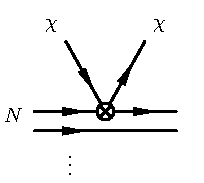
\includegraphics[scale=1]{figs/nuc-curr}
\hspace*{0.3cm}
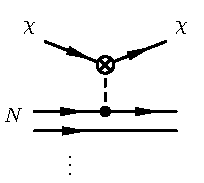
\includegraphics[scale=1]{figs/mes-curr}
\hspace*{0.3cm}
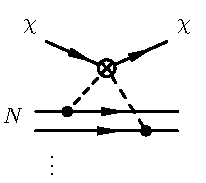
\includegraphics[scale=1]{figs/mes-curr-nlo1}
\hspace*{0.3cm}
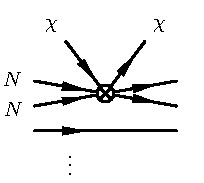
\includegraphics[scale=1]{figs/nuc-curr-nlo}
\caption[Chiral perturbation theory for DM]{\label{fig:DM:ChPT}\it The first and second panel from the left show the diagrams for DM-nucleus scattering that are of leading order in chiral counting. The long distance (third diagram) and short distance (fourth diagram) two nucleon interactions are examples of higher order correction in chiral counting. The effective DM--nucleon and DM--meson interactions is denoted by a circle, the dashed lines denote mesons, and the dots represent the remaining $A-2$ nucleon lines.  Adapted from \cite{Bishara:2016hek} ($\copyright$IOP Publishing, reproduced with permission).}
\end{figure}

There are several general lessons that one can draw from the above chiral expansion~\cite{Bishara:2017pfq,Bishara:2016hek,Chiral-EFT-DM}. 
Perhaps most importantly,  the chirally-leading contributions to DM scattering involve only scattering on a single nucleon. Such contributions are of two types. If DM couples to a nucleon through a point interaction (the first diagram in fig.~\ref{fig:DM:ChPT}) the resulting non-relativistic coefficient $c_i^N$ in \eqref{eq:LNR} is $q$-independent. 
If instead DM  interacts with a nucleon by emitting an off-shell light meson, $\pi^0$ or $\eta$, or a photon (the second diagram in fig.~\ref{fig:DM:ChPT}), this results in light meson or photon poles, $c_i^N\propto 1/(q^2 +m_\pi^2)$ and $c_i^N\propto 1/\mb{q}^2$.   
An explicit example of the former was encountered in eq.~\eqref{eq:c4N:c6N:axial}. 
The pole counteracts ${\mathcal O}(q^2)$ suppressions.  Therefore, the proper description of leading non-relativistic DM interactions in $\Lag_{\rm NR}$, eq.~\eqref{eq:LNR},  requires us to keep operators with up to two derivatives (but not with more derivatives).

For a number of DM EFT operators the hadronization is quite simple, and results, at leading order in the chiral expansion, in just one non-relativistic operator. For instance,\footnote{We define the form factors following~\cite{Bishara:2017pfq}:
\beq \langle N'| \big\{\bar q \gamma^\mu q, m_q \bar q   q,\frac{\alpha_{\rm s}}{8\pi} G^{a\mu\nu}\tilde G^a_{\mu\nu}, m_q \bar q \sigma^{\mu\nu} q \} |N\rangle= \bar u_N'\big\{F_1^{q/N}\gamma^\mu+\cdots, F_S^{q/N},F_G^{N}, F_{T,0}^{q/N} \sigma^{\mu\nu} +\cdots \big\}u_N,\eeq 
where the ellipses denote the form factors that, for the operators we are considering, contribute only at subleading orders in chiral expansion. At zero momentum exchange the vector currents count the number of
valence quarks in the nucleon. Hence, the normalization of the Dirac
form factors for the proton is $ F_1^{u/p}(0)=2,  F_1^{d/p}(0)=1, F_1^{s/p}(0)=0$. The scalar form factors $F_S^{q/N}$
evaluated at $q^2=0$ are conventionally referred to as the nuclear sigma
terms, $F_S^{q/N}(0)= \sigma_q^N\sim {\mathcal O}(10\text{s~MeV})$.  
  Another common notation
is $\sigma_q^N=m_Nf_{Tq}^{N}$. The trace of the stress-energy tensor gives for the gluonic form factor
$F_G^{N}(0)=-\frac{2}{27}(m_N-\sum_q \sigma_q^N)$. The tensor form factor at zero recoil is given by
$
F_{T,0}^{q/p}(0)=m_q A_{T,10}^{q/N}(0)=m_q  g_{T}^{q}$,
where the values of the tensor charges  $g_{T}^q(\mu)$ are listed below eq.~\eqref{eq:c4:tensor}. The arrows in \eqref{eq:Ops:NR} denote the replacements of operators to be done in \eqref{eq:lightDM:Lnf5}, which then give $\Lag_{\rm NR}$ in \eqref{eq:LNR}.
} 
\beq
\label{eq:Ops:NR}
\Op_{1,q}^{(6)}\to F_1^{q/N} {\mathcal O}_1^N, \qquad 
\Op_{1}^{(7)}\to  F_G^{N}{\mathcal O}_1^N, \qquad
\Op_{5,q}^{(7)}\to F_S^{q/N}{\mathcal O}_1^N\,, \qquad
\Op_{9,q}^{(7)}\to  8 F_{T,0}^{q/N} {\mathcal O}_4^N\,,
\eeq
where all the form factors are evaluated at zero momentum transfer, $q^2=0$,
resulting in constant non-relativistic coefficients, $c_{1,4}^N$. The non-relativistic reductions of vector-vector DM interactions ($\Op_{1,q}^{(6)}$, eq.~\eqref{eq:dim6EW:Q1Q2:light}), as well as scalar DM interactions with  gluons and quarks ($\Op_{1}^{(7)}$, $\Op_{5,q}^{(7)}$ in eq.s \eqref{eq:dim7:Q3Q4:light}, \eqref{eq:dim7:Q3Q4:light}),  all lead to SI scattering (they generate $c_1^N$). These were used in section \ref{sec:benchmark:models} to obtain the SI scattering cross sections for Higgs-mediated, eq.~\eqref{eq:Higgs:sigmaSI}, and for $Z$-mediated DM interactions, eq.~\eqref{eq:DDZmediated}. 
The tensor-tensor operator $\Op_{9,q}^{(7)}$, eq.~\eqref{eq:dim7EW:Q9Q10:light}, on the other hand, leads to spin-dependent scattering (it generates $c_4^N$, see also eq.~\eqref{eq:tensor:int}). 

\smallskip

On the other hand,
the chirally-leading hadronization  is quite complicated
for the magnetic moment operator $\Op_{1}^{(5)}$ in eq.~\eqref{eq:dim5:nf5:Q1Q2:light} and 
for the axial-axial operator $\Op_{4,q}^{(6)}$ in eq.~\eqref {eq:dim6EW:Q3Q4:light}:
\begin{align}
\begin{split}
\label{eq:Q15}
\Op_{1}^{(5)}\to& -\frac{\alpha}{2\pi} Q_{N}\Big(
\frac{1}{M}{\mathcal O}_1^N-4 \frac{m_N}{ q^2}
{\mathcal O}_5^N\Big)-\frac{2\alpha}{\pi
}\frac{\hat \mu_N}{m_N}\Big({\mathcal O}_4^N-\frac{m_N^2}{ q^2}
{\mathcal O}_6^N\Big)\,, 
\end{split}
\\
\begin{split}
\label{eq:Q46}
\Op_{4,q}^{(6)}\to& -4 F_A^{q/N} {\mathcal O}_4^N+F_{P'}^{q/N} {\mathcal O}_6^N,
\end{split}
\end{align}
where $Q_N$ ($\hat \mu_N$) is the nucleon's electric charge 
(magnetic moment, $\hat \mu_p\approx 2.793$, $\hat \mu_n\approx -1.913$),  
while $F_A^{q/N}(q^2), F_{P'}^{q/N}(q^2)$ are the form factors for the axial current
\beq
\label{axial:form:factor}
\langle N'|\bar q \gamma^\mu \gamma_5 q|N\rangle=\bar u_N'\Big[F_A^{q/N}(q^2)\gamma^\mu\gamma_5+\frac{1}{2m_N}F_{P'}^{q/N}(q^2) \gamma_5 q^\mu\Big]u_N\,.
\eeq
The form factors parametrise the response of a nucleon to an axial-vector probe $\bar q \gamma^\mu \gamma_5 q$ that gives  a four-momentum $q^\mu$ kick to the initial nucleon in a state $| N\rangle\equiv |
N(k_1)\rangle $, transforming it into the final nucleon state $\langle N'|\equiv\langle N(k_2)| $.  
The expressions in eq.s~\eqref{eq:Q15}, \eqref{eq:Q46} 
illustrate that a single relativistic operator can result in several non-relativistic operators $\Op_i^N$, and that the coefficients $c_i^N$ multiplying them depend on $q^2$. 
This $q^2$ dependence is  known. 
Let us first focus on the case of DM magnetic moment, eq.~\eqref{eq:Q15}. 
Tree-level photon exchange between DM and a nucleon gives rise to terms with $1/{q}^2$ poles (multiplying $\Op_{5,6}^N$ operators), as expected for a propagating photon. It also leads to ${q}^2$-independent contact terms (multiplying $\Op_{1,4}^N$ operators) because the magnetic moment interaction in eq.~\eqref{eq:dim5:nf5:Q1Q2:light} contains derivatives that can completely cancel the photon pole. The photon poles in eq.~\eqref{eq:Q15} then only multiply the operators with two derivatives, i.e., the two operators $\Op_{5,6}^N$ that are $\Op(q^2)$. All four terms in eq.~\eqref{eq:Q15} are thus of the same parametric order. Which contribution is the most important numerically, the SI contribution from $\Op_1^N$ or the SD contributions from $\Op_{4,5,6}^M$, depends on the type of nucleus and on the DM mass $M$. 

\smallskip

Finally, we turn to the hadronization of the axial-axial operator, eq.~\eqref{eq:Q46}. The $q^2$ dependence in the form factors $F_{A,P'}^{q/N}(q^2)$ leads to the $q^2$ dependence in the non-relativistic coefficients $c_{4,6}^N$  in $\Lag_{\rm NR}$, eq.~\eqref{eq:LNR}. We only need the chirally-leading behaviour, which amounts to expanding in small $q^2/m_N^2$
\beq
\label{eq:FA:FP':expand}
F_A^{q/N}(q^2)=\Delta q_N+\cdots,  \qquad F_{P'}^{q/N}(q^2)=\frac{m_N^2}{m_\pi^2+q^2} a_{q/N}+\frac{m_N^2}{m_\eta^2+q^2} \tilde a_{q/N} +\cdots.
\eeq
Both the value of $F_A^{q/N}(0)=\Delta q_N$ and the residua of the $\pi$ and $\eta$ poles, $a_{u/p}=-a_{d/p}=2 g_A$, $a_{s/p}=0$, $\tilde a_{u/p}=\tilde a_{d/p}=-\tilde a_{s/p}/2=2\big(\Delta
u_p+\Delta d_p-2 \Delta s_p\big)/3 $, are related to the axial charges of the proton,  $\Delta u\equiv \Delta u_p=0.897(27)$, $\Delta d\equiv \Delta d_p=-0.376(27)$, 
$\Delta s\equiv \Delta s_p=-0.031(5)$, where $g_A=\Delta u-\Delta d=1.2723(23)$  \cite{Bishara:2017pfq}. The expressions for neutrons are obtained by making the replacements $p\to n, u\leftrightarrow d$ (no change is implied for
$g_A$).  The resulting explicit forms of $c_{4,6}^N$, neglecting the $\eta$ pole, 
are given in eq.~\eqref{eq:c4N:c6N:axial}. 
The leading ChPT expression for $c_{4}^N$ is $q^2$ independent, i.e., the $\Op_4^N$ term corresponds to the first diagram in  fig.~\ref{fig:DM:ChPT}. The $c_6^N$ contains the light meson poles, and is thus given by the second diagram in fig.~\ref{fig:DM:ChPT}.  The pion pole enhancements compensates the $\Op(q^2)$ suppression in the $\Op_6^N$ operators, and thus the two terms in eq.~\eqref{eq:Q46} are of parametrically similar size. 


\bigskip

This completes our discussion of leading nonperturbative matching. The matching expressions in eq.s~\eqref{sys:tonuclei} get corrected at higher orders in chiral expansion. 
Going to higher orders requires inclusion of DM interactions with two nucleons. 
An example is the third diagram in fig.~\ref{fig:DM:ChPT}, where DM scatters off a pion exchanged between two nucleons. Such `long distance' contributions are expected to be most important for axial-vector--vector, scalar--scalar and pseudo-scalar--scalar forms of DM/SM interactions,  
for which they enter as ${\mathcal O}(q)$ corrections in chiral counting. In contrast,  the short distance two-nucleon contributions, 4th diagram in fig.~\ref{fig:DM:ChPT}, 
are nominally only an ${\mathcal O}(q^3)$ correction. 
However, non-perturbative renormalizations can change these scaling. Resumming ladder diagrams with long distance insertions may require counter-terms (short distance) contributions that are formally of higher order. This is understood for $np, nn, pp$ scattering to be a consequence of a new scale appearing in the low energy phenomenology --- the large scattering length and the existence of bound states, such as deuteron \cite{Chiral-EFT}. It can also be understood as a change of order due to divergence  of two-nucleon wave function at the origin \cite{PavonValderrama:2014zeq}. Such effects were found to be important for neutrino-less double-beta decays, where the long distance two body interaction is due to a tree level exchange of a light neutrino \cite{Chiral-EFT-0beta}. Two-body current contributions were included for scalar DM interactions in the mean field approximation in \cite{2body:currents:DM:scattering} and found to be numerically relevant only when the chirally leading terms have large cancellations. For most applications the chirally leading calculations thus suffice, especially in view of sizable systematic errors in the evaluation of some of the nuclear response functions that we discuss next. 



\subsubsection{Nuclear response functions} 
\index{Nuclear response functions}

Restricting the discussion to the chirally-leading order, 
the cross section for the DM scattering on a nucleus is obtained by taking the matrix element of DM interactions with single nucleon currents in the non-relativistic effective Lagrangian $\Lag_{\rm NR}$,  eq.~\eqref{eq:LNR},
\beq
\big|\mathscr{A}\big|^2_{\rm nucleus, NR}=\sum_{i,j}\sum_{N,N'} c_i^{N} c_j^{N'*}\langle A|\Op_i^N|A\rangle \langle A|\Op_j^{N'}|A\rangle,
\eeq 
where the sum runs over $N,N'=n,p$, and all the non-relativistic operators with up to two derivatives, $i,j=1,\ldots,14$ (see eq.s~\eqref{eq:O1pO2p}, \eqref{eq:O5pO6p} and  \arxivref{1308.6288}{Anand et al. (2013)}~\cite{Anand:2013yka}). 
The high-energy particle physics is encoded in the non-relativistic coefficients $c_i^{N}$. 
The products of nuclear matrix elements $\langle A|\Op_i^N|A\rangle \langle A|\Op_j^{N'}|A\rangle$, on the other hand, depend only on nuclear physics, and can be calculated once and for all. Once averaged over nuclear spin (we consider only scatterings on unpolarized nuclei), this results in eight nuclear response functions needed for the description of DM scattering on nucleus at leading order in chiral expansion. The nuclear response functions depend on $q=|\vec q\,|$ and have the
approximate scalings
\begin{equation}\label{eq:scaling}
W_M\sim {\mathcal O}(A^2)\,, \qquad W_{\Phi'' M} \sim {\mathcal O}(A), \qquad W_{\Sigma'}, W_{\Sigma''},
W_{\Delta}, W_{\Delta\Sigma'},W_{\tilde \Phi'}, W_{\Phi''}\sim{\mathcal O}(10^{-2})-{\mathcal O}(1)\,.
\end{equation}

The $W_{\Sigma'}, W_{\Sigma''}, W_{\Delta}$, and $W_{\Delta\Sigma'}$
response functions depend strongly on the detailed properties of
nuclei, for instance, whether or not these have an unpaired nucleon in the outer shell. 
Here:
\begin{itemize}
\item[$\ast$] $W_{\Sigma',\Sigma''}$ encode the spin content
of the nucleus discussed in section~\ref{sec:SD}.
\item[$\ast$] $W_{\Delta}$ encodes the average angular momentum in the nucleus, 
and $W_{\Delta\Sigma'}$ the interference of the two. 
\item[$\ast$]  $W_{\tilde \Phi'}$ and $W_{\Phi''}$ encode the size of spin-orbit coupling in the nucleus. 
They can thus differ drastically between different isotopes of the
same element. 
\item[$\ast$]  $W_M$ encodes the coherent scattering
enhancement, ${\mathcal O}(A^2)$, where $A$ is the atomic mass number.
\item[$\ast$] $W_{\Phi'' M}$ gives the interference between spin-orbit coupling operator and the coherent scattering. 
\end{itemize}
The coherence is achieved in the long-wavelength limit, $q\to 0$, where
DM scatters coherently on the whole nucleus, for instance, due to the
$\Op_1^N$ contact interaction (see also the discussion in section~\ref{sec:SI}). 

 The DM/nucleus scattering cross section is given by
\cite{Anand:2013yka},
\begin{equation}
\label{eq:dsigmadER}
\begin{split}
\frac{d\sigma^A}{d E_R} = \frac{2 m_A}{(2 J_A+1)v^2}\sum_{\tau,\tau'}
\bigg[ & R_M^{\tau\tau'}W_M^{\tau\tau'} +
  R_{\Sigma''}^{\tau\tau'}W_{\Sigma''}^{\tau\tau'} +
  R_{\Sigma'}^{\tau\tau'}W_{\Sigma'}^{\tau\tau'}  + \frac{{q}^{2}}{m_N^2}\Big(R_{\Delta}^{\tau\tau'}W_{\Delta}^{\tau\tau'}+
        \\ &
  +R_{\Delta
    \Sigma'}^{\tau\tau'}W_{\Delta\Sigma''}^{\tau\tau'}
  +R_{\tilde \Phi'}^{\tau\tau'}W_{\tilde \Phi'}^{\tau\tau'}+
    R_{\Phi''}^{\tau\tau'}W_{\Phi''}^{\tau\tau'} +R_{\Phi'' M}^{\tau\tau'}W_{\Phi'' M}^{\tau\tau'}
    \Big)\bigg]\,. 
\end{split}
\end{equation}
Here, $E_R$ is the recoil energy of the nucleus, $m_A$ the mass of the
nucleus, $J_A$ its spin, and $v$ the initial DM velocity in the lab
frame. The kinematical factors contain the $c_i^N$ coefficients,
\begin{eqnsystem}{sys:nuclkin}
\label{eq:RM}
R_M^{\tau\tau'}&=&c_1^\tau c_1^{\tau'}+\frac{1}{4}\frac{{q}^{2}}{m_N^2} v_T^{2} c_5^\tau c_5^{\tau'} +\cdots\,,
\\
R_{\Sigma''}^{\tau\tau'}&=&\frac{1}{16}\Big(c_4^{\tau}c_4^{\tau'}+\frac{{q}^{2}}{m_N^2}\big(c_4^\tau c_6^{\tau'}+c_6^\tau c_4^{\tau'}\big) + \frac{{q}^{4}}{m_N^4}c_6^\tau c_6^{\tau'}\Big)\,,
\\
\label{eq:RSigma}
R_{\Sigma'}^{\tau\tau'}&=&\frac{1}{16}c_4^\tau c_4^{\tau'}+\cdots \,, \qquad
R_{\Delta}^{\tau\tau'}=\frac{1}{4}\frac{{q}^{2}}{m_N^2}c_5^\tau c_5^{\tau'}+\cdots\,,\qquad
R_{\Delta\Sigma'}^{\tau\tau'}=\frac{1}{4}c_5^\tau c_4^{\tau'}+\cdots\,,
\end{eqnsystem}
where $ \vec v_T=\big(\vec p_1+\vec p_2\big)/2{M}-\big(\vec k_1+\vec k_2\big)/2{m_A}$, with $\vec p_{1(2)}$ and $\vec k_{1(2)}$  the incoming (outgoing) DM and nuclear three-momenta, respectively.
Note that for heavy nuclei such as xenon $ \vec v_T\sim v \sim {\mathcal O}(10^{-3})$ is much smaller than the equivalent perpendicular velocity $v_\perp\sim {\mathcal O}(0.1)$ 
for the scattering on nucleons, see also the discussion surrounding eq.~\eqref{eq:O5pO6p}. 
For light nuclei, on the other hand, $ \vec v_T\sim v_\perp$. The sum in eq.~\eqref{eq:dsigmadER} is over isospin,
$\tau,\tau'=0,1$, so that
\begin{equation}
c_i^{0(1)}=\frac{1}{2}\big(c_i^p\pm c_i^n\big)\,.
\end{equation} 
In eq.s~\eqref{sys:nuclkin} we set $J=1/2$ for simplicity and only displayed the dependence on the coefficients for the non-relativistic operators we focused on in the previous subsection, eq.s~\eqref{eq:O1pO2p}, \eqref{eq:O5pO6p}. 
The complete expressions for $R_i^{\tau\tau'}$ can be found in  \arxivref{1308.6288}{Anand et al. (2013)} in~\cite{Anand:2013yka}.

\smallskip

The form of the kinematical functions \eqref{eq:RM}-\eqref{eq:RSigma} agrees with the chiral counting we discussed in the previous subsection. 
The coefficients $c_{5,6}$, enhanced by a $1/{q}^2$ pole, 
come suppressed by either ${q}^2/m_N^2$ or $v_T^2$, 
and thus lead to parametrically similar contributions as the $c_1$ and $c_4$ coefficients. 
The new ingredient that was not captured by the chiral counting is the possibility of coherent enhancement of the nuclear response functions, eq.~\eqref{eq:scaling}. Both $\Op_1^N$ and $\Op_5^N$ operators contain the nuclear number operator $1_N$ and thus exhibit coherent enhancement in eq.~\eqref{eq:RM}. 
However, for $\Op_5^N$ all the nucleons need to scatter in the same direction, converting the individual $\vec v_\perp$ factor to their sum, resulting in a much smaller $v_T$ suppression, effectively negating the coherent enhancement. 

\smallskip

The precision of the cross section prediction for the DM scattering on nuclei  in eq.~\eqref{eq:dsigmadER} depends in large part on  how well the nuclear response functions can be predicted. 
While ab initio nuclear calculations are possible for light nuclei, 
and for some more symmetric not-so-light nuclei such as $^{40}$Ca, 
this is not the case for heavy nuclei such as Xe, W, where various approximations are needed. 
Typically, calculations are done using the shell model with different choices for nuclear potentials.  \arxivref{1308.6288}{Anand et al. (2013)} in \cite{Anand:2013yka} provided shell model calculations of response function $W_i$ for most nuclei used in direct detection experiments. Alternative calculations for spin independent response functions are available in~\cite{Hoferichter:2018acd} (though not using the $W_i$ notation, but also including two body current corrections). The systematic errors of these calculations are  not easy to estimate, though some guidance is provided by comparing the results of different groups, when these are available. For $W_M$ the precision of a few percent is possible, while for other $W_i$ the errors are typically expected to be much larger. 


\subsubsection{Modifications for light mediators}
Throughout this section we assumed that the mediators are heavier than a few GeV, so that the use of DM EFT Lagrangian, eq.~\eqref{eq:lightDM:Lnf5}, is warranted. 
What happens, if mediators are lighter? Since light mediators are necessarily color neutral 
(they do not feel the strong force), the required changes to the above formalism are rather straightforward. The point interaction between DM and SM fields gets replaced by long range interactions. That is, the Wilson coefficients in \eqref{eq:lightDM:Lnf5} become $q^2$ dependent. Apart from this modification all the results carry through unchanged. A concrete example of this type is the dark photon mediator. The resulting $q^2$-dependent $c_1^N$ coefficient, eq.~\eqref{eq:c1p:c1n:darkphoton}, can be used directly in the expression for the differential cross section for DM scattering on nuclei, eq.~\eqref{eq:dsigmadER}.

\subsection{Numerical codes}
A number of computer codes compute DM direct detection scattering rates. {\tt DirectDM} \cite{Bishara:2017nnn} in combination with {\tt DMFormFactor} \cite{Anand:2013yka} calculates the scattering cross sections for general DM interactions with the SM, based on the EFT approach discussed in section \ref{sec:Effective:operators}. This includes the SI and SD scattering, but also allows for more general interactions, starting either from the theory of DM interactions with quarks, gluons and photons, or from a non-relativistic description of DM interactions with nucleons. Another package with a similar scope is {\tt ChiralEFT4DM} \cite{Hoferichter:2018acd}. {\tt MadDM}  \cite{MadDM} calculates the SI and SD scattering rates starting from a Lagrangian for DM interactions with the SM. It is a plug-in for the very popular automatized matrix element generator {\tt MadGraph5\_aMC\@NLO} \cite{Alwall:2014hca}, and as such can utilize other popular tools such as {\tt FeynRules} \cite{Alloul:2013bka} that takes as input the DM interaction Lagrangian. 
The code {\tt micrOMEGAs} \cite{0803.2360} calculates the SI and SD scattering rates for a general set of DM models for which these are the leading scattering rates, and also provides the recasting of limits from experimental results to the space of DM couplings \cite{Belanger:2020gnr}. Such recasting can also be achieved using {\tt DarkBit} \cite{GAMBITDarkMatterWorkgroup:2017fax}.


\section{Scattering on electrons}\index{Direct detection!on $e$}
\label{sec:direct:electrons}

Scattering of DM on electrons is most important for probing sub-GeV DM, for which the mass of the target --- the electron --- is closer to the mass of DM and thus the energy transfer is most efficient. Lighter DM implies smaller kinetic energy, and thus smaller deposited energy and momenta exchanges in the scattering events. The deposited energy can even be comparable to the energy excitations of the collective modes in the target materials, such as plasmons or magnons, which then need to be taken into account. This is especially true for the absorption of a very light, ${\mathcal O}(10\text{\,eV})$, DM  in the material in which case also the kinematics matches with such collective mode excitations. The resulting current constraints on SI DM scattering on electrons are given in fig.~\ref{fig:DDSIelec:bounds}.

\begin{figure}[t]
\begin{center}
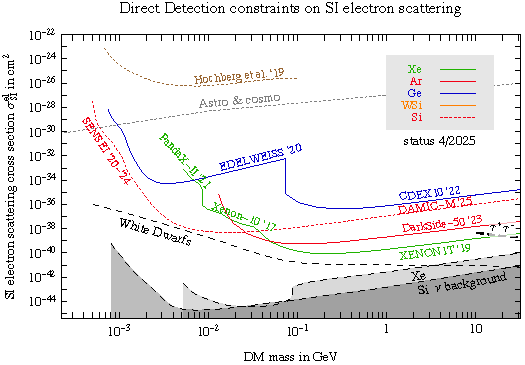
\includegraphics[width=0.72 \textwidth]{figs/Direct25SIelec}
\end{center}
\caption[Bounds on $\sigma_{\rm SI}^{\rm el}$]{\em\label{fig:DDSIelec:bounds} 
The same as in fig.~\ref{fig:sigmaSIbound} (bottom), but for bounds   from underground detectors on the spin-independent direct detection cross section for {\bfseries scattering on electrons} 
$\sigma_{\rm SI}^{\rm el}$ in the limit of heavy mediators, see eq.~\eqref{eq:sigma:el}. The estimate for neutrino backgrounds on Xe and Si targets is taken from \arxivref{2312.04303}{Carew et al. (2024)} in \cite{nubckg}  (see also section~\ref{nubck}). The White Dwarf bounds assume annihilating DM, see section \ref{sec:CaptureWD}. Black dashed line with the $\tau^+\tau^-$ label indicates the bound due to possible $\text{DM}+\text{DM}\to \tau^+\tau^-$ annihilation that would produce neutrinos from the Sun,
see section~\ref{sec:DMnu}. The Hochberg et al.\,'19 bound is obtained using superconducting nanowires, see section \ref{sec:novel:material} and \cite{DM:electron:superconductors:nanowiresHochberg}. The astrophysical and cosmological bound is taken from \arxivref{2107.12377}{Buen-Abad et al.~(2022)} \cite{SIMP}, see section \ref{sec:SIMP}.
}
\end{figure}
 
 To be able to describe the effects of scattering on bound electrons we need to extend the formalism of section \ref{sec:DMscatt:nuclei}, used for DM scattering on nuclei, such that it applies to the case of scattering of DM on bound electrons.\footnote{We follow the review \cite{dm:light:review}, where many more details can be found.} Starting with the Fermi's Golden rule the event rate per unit target mass, $R_{\rm ev}=dN_{\rm ev}/dt \times 1/m_T$, for DM scattering in a target with a volume $V$ and mass $m_T$ is given by \cite{SI:DM:electron:scattering,dm:light:review} 
 \beq
\label{eq:Fermi:rule}
R_{\rm ev}=\frac{1}{\rho_T}  \int
dn_{\rm DM}(\vec v)  \frac{V d^3 \vec p_2}{(2\pi)^3} \sum_f \big|\langle f, \vec p_2\big| H_{\rm int}\big|i, \vec p_1\rangle \big|^2 2\pi \delta(E_f-E_i+E_2-E_1),
 \eeq
 where $\rho_T=m_T/V$ is the mass density of the target material, 
 $\vec p_{1(2)}$ and $E_{1(2)}$ are the incoming (outgoing) DM  three momenta and energies, $H_{\rm int}$  the non-relativistic Hamiltonian describing DM--electron interactions,  $|i\rangle$ and $|f\rangle$ are the initial and final state of the detector with energies $E_i$, $E_f$, respectively, while $n_{\rm DM}(\vec v)$ is the volume density of DM particles with velocity $\vec v=\vec p_1/M$, see eq.~\eqref{eq:NevER}. The wave functions are unit normalized, $\langle i|i\rangle=\langle f |f\rangle= \langle \vec p_i|\vec p_i\rangle=1$. The factor $Vd^3\vec p_2/(2\pi)^3$ gives the density of states for the outgoing DM plane wave. The event rate is also proportional to the number of DM particles, $V \int dn_{\rm DM}(\vec v)$. Normalizing to the target mass, $m_T$, then results in the appearance of the $\int dn_{\rm DM}(\vec v)/\rho_T$ factor in eq.~\eqref{eq:Fermi:rule}. 
 
Eq.~\eqref{eq:Fermi:rule} generalizes the expression for DM scattering on a single nucleus, eq.~\eqref{eq:NevER}, 
by not requiring that the scattering is $2\to 2$ and not imposing the corresponding kinematic constraints, 
except for energy conservation. 
Eq.~\eqref{eq:Fermi:rule} therefore allows for DM scattering on many electrons at the same time (on collective modes, the quasi-particles). 
The simplification in the DM/electron scattering problem is that for most applications both DM and electrons are non-relativistic so that one can use the usual non-relativistic quantum mechanics to evaluate the matrix element in eq.~\eqref{eq:Fermi:rule}. However, the electrons are inside the medium, in a strongly interacting regime, so that the problem is far from a simple one. 
Luckily, one can use the tools developed for condensed matter problems to make headway.
 
 \smallskip
 
 The non-relativistic DM/electron interaction Hamiltonian takes a form of a product of DM and electron currents
 \beq
 H_{\rm int}=\int \frac{d^3\vec q}{(2\pi)^3} e^{i\vec q \cdot (\vec r_{\rm el}-\vec r_{\rm DM})} \sum_a c^{\rm el}_a (q)\,\, \Op_{\rm DM}^a \times \Op_{\rm el}^a,
 \eeq
 where the various operators are the same  as for the non-relativistic DM interactions with the nucleons, eq.~\eqref{eq:LNR}, but with nucleons replaced by electrons: $m_N\to m_e$ and $\vec S_N\to \vec S_e$. 
 The matrix elements therefore factorize into the DM and electron (target) parts, 
 $\langle f, \vec p_2\big| H_{\rm int}\big| i, \vec p_1\rangle\sim  c_{\rm el}^a \langle  \vec p_2\big| \Op_{\rm DM}^a\big| \vec p_1\rangle \langle f \big| \Op_{\rm el}^a\big| i \rangle$. 
 The DM matrix elements $\langle  \vec p_2\big| \Op_{\rm DM}^a \big| \vec p_1\rangle$ and the values of the coefficients $c_{\rm el}^a (q)$ change from one DM model to another. 
 In particular, for heavy mediators $c_{\rm el}^a$  are constant, while for light mediators  they are $q$-dependent due to the propagator of the light mediator,  signalling that in this case  $H_{\rm int}$ is nonlocal. 
 For instance, a tree level exchange of a dark photon  induces the operator ${\mathcal O}_1^{\rm el}= 1_{\rm DM} 1_{\rm el}$ with a coefficient (see also section~\ref{sec:VectorPortal})
 \beq
 c^{\rm el}_1 (q)=-\frac{\varepsilon e g_{\rm D}}{ q^2+m_{A'}^2},
 \eeq
 where $\varepsilon$ is the kinetic mixing parameter, $\Lag\supset \varepsilon F_{\mu\nu}'F^{\mu\nu}/2$, which induces the coupling of strength $\varepsilon e$ between electrons and the dark photon,  while $g_D$ is its coupling to DM. If  the dark photon mass $m_{A'}$ is comparable to the typical momentum exchange, the $ q$ dependence in $c^{\rm el}_1 (q)$ cannot be neglected. 
 
 \smallskip
 
Unlike the $c^{\rm el}_a (q)$ coefficients, which change model to model, the response of the target material, encoded in $|\langle f \big| \Op_{\rm el}^a\big| i \rangle |^2$ and in similar interference terms between different operators, can in principle be calculated once and for all. This has been performed for a number of operators and materials, such as the isolated atom and crystals, in~\cite{DM:electron:EFT}. However, by far the main focus of the research so far has been on spin-independent DM--electron scattering, partially because the most popular sub-GeV DM physics models lead to SI scattering, but also because the response to SI scattering can be related to the leading behaviour of material under electromagnetic probes and is thus better explored.   

From now on we thus limit the discussion to the SI interaction
 \beq
 H_{\rm int}^{\rm SI}= \int \frac{d^3\vec q}{(2\pi)^3} e^{i\vec q \cdot (\vec r_{\rm el}-\vec r_{\rm DM})} c_1^{\rm el} (q) 1_{\rm DM} 1_{\rm el},
 \eeq
for which the scattering rate can be written as 
 \beq
\label{eq:Fermi:rule:v2}
R_{\rm ev}^{\rm SI}=\frac{1}{\rho_T}  \int
dn_{\rm DM}(\vec v)  \int \frac{ d^3 \vec q}{(2\pi)^3}  d\omega \frac{\pi  \bar \sigma (q)}{\mu_e^2} \delta (\omega+E_2-E_1) S(\vec q, \omega),
 \eeq
 where $\mu_e$ is the reduced mass of the electron/DM system, $\mu_e=m_e M/(m_e+M)$. The quantity
 \beq
 \label{eq:sigma:el}
 \bar \sigma (q)=\frac{\mu_e^2}{\pi} [c_1^{\rm el}(q)]^2,
 \eeq
 reduces to the SI cross section for scattering of DM on free electrons, $\sigma_{\rm SI}^{\rm el}$, in the limit of a heavy mediator, $c_1^{\rm el}(q)\to c_1^{\rm el}(0)$. In general, however, it is $q$-dependent, and encodes the strength of the DM/electron interactions. In the literature, a common notation is to introduce the fiducial cross section $\sigma_T\equiv \bar \sigma(q_0)$ at a fixed momentum $q_0$, typically the inverse Bohr radius, $q_0=1/a_0=\alpha m_e\simeq 3.7$ keV, and write  $\bar \sigma (q)=\sigma_T F_{\rm DM}^2(q)$, where  $F_{\rm DM}(q)\equiv c_1^{\rm el}(q)/c_1^{\rm el}(q_0)$ is the {\em DM form factor}. This is somewhat of a misnomer since the $q$ dependence of $F_{\rm DM}(q)$ does not signal that DM is a composite object but rather comes from propagation of light mediators. For heavy mediators $F_{\rm DM}\to 1$, while for light mediators $F_{\rm DM}\to (q_0/q)^2$.
 
\smallskip 
 
The {\em dynamic structure factor}, \index{Dynamic structure factor}
 \beq
 \label{eq:S:electron:general}
S(\vec q, \omega)=\frac{2\pi}{V} \sum_f \big|\langle f \big| \sum_k e^{i\vec q \cdot \vec r_{k}}\big| i \rangle \big|^2 \delta(E_f-E_i-\omega),
 \eeq
gives the response of the material to the probe $ e^{i\vec q \cdot \vec r_{\rm el}} 1_{\rm el}$, resulting in the sum $\sum_k$ over all the electrons in the target. The  variable $\omega$ in eq.~\eqref{eq:Fermi:rule:v2} gives the energy deposited in the material during the scattering event. In deriving eq.~\eqref{eq:Fermi:rule:v2} from \eqref{eq:Fermi:rule} the conservation of DM three-momenta, $\vec q=\vec p_1-\vec p_2$ was used to convert the $d^3 \vec p_2 $ integral to an integral over $d^3\vec q$. However, the derivation of eq.~\eqref{eq:Fermi:rule:v2} did not assume the conservation of the three-momentum in the target. In fact, since the crystal lattice breaks translation invariance, the eigenstates of the target are in general not  eigenstates of momentum. 

For scattering on a dilute non-relativistic free electron gas at negligible temperature (i.e., for electrons essentially at rest) the structure function is given by
 \beq
 \label{eq:S:free:el}
S(\vec q, \omega)={2\pi}n_e \,\delta\Big(\omega- \frac{q^2}{2m_e}\Big),
 \eeq
where $n_e$ is the electron number density. 
The delta function in eq.~\eqref{eq:S:free:el} ensures that the deposited energy $\omega$ satisfies the non-relativistic dispersion relation. The limit of scattering on free electrons is approached for large momenta exchanges, $q\gg 1/a_0= \alpha m_e=3.73$~keV (the inverse of Bohr radius $a_0$ represents the typical extent of the electron wave-function)  
and for energy deposits $\omega \gg \alpha^2 m_e$ (the typical atomic electron binding energy). 
That is, for $q\gtrsim {\mathcal O}(\text{keV})$ and $\omega \gtrsim {\mathcal O}(10 \text{\,eV})$ the response of the material to the DM/electron interactions peaks around the free electron dispersion $\omega=q^2/2 m_e$, 
shown schematically as  the green band in fig.~\ref{fig:DM:electrons} (left). The momenta exchanges and energy deposits of this size are achieved only for scattering of heavy enough DM, with mass above ${\mathcal O}(\rm{GeV})$.  
For lighter DM masses it is important to take into account that the electrons are bound. First of all, many of the materials have energy gaps so that a minimal DM kinetic energy is required to be able to excite electrons, which then implies that there is a lower limit on the DM masses that can be probed by a given detector material. For very light sub-GeV DM, i.e., with a sub-MeV mass, the collective effects also become important. 




\begin{figure}[t]
$$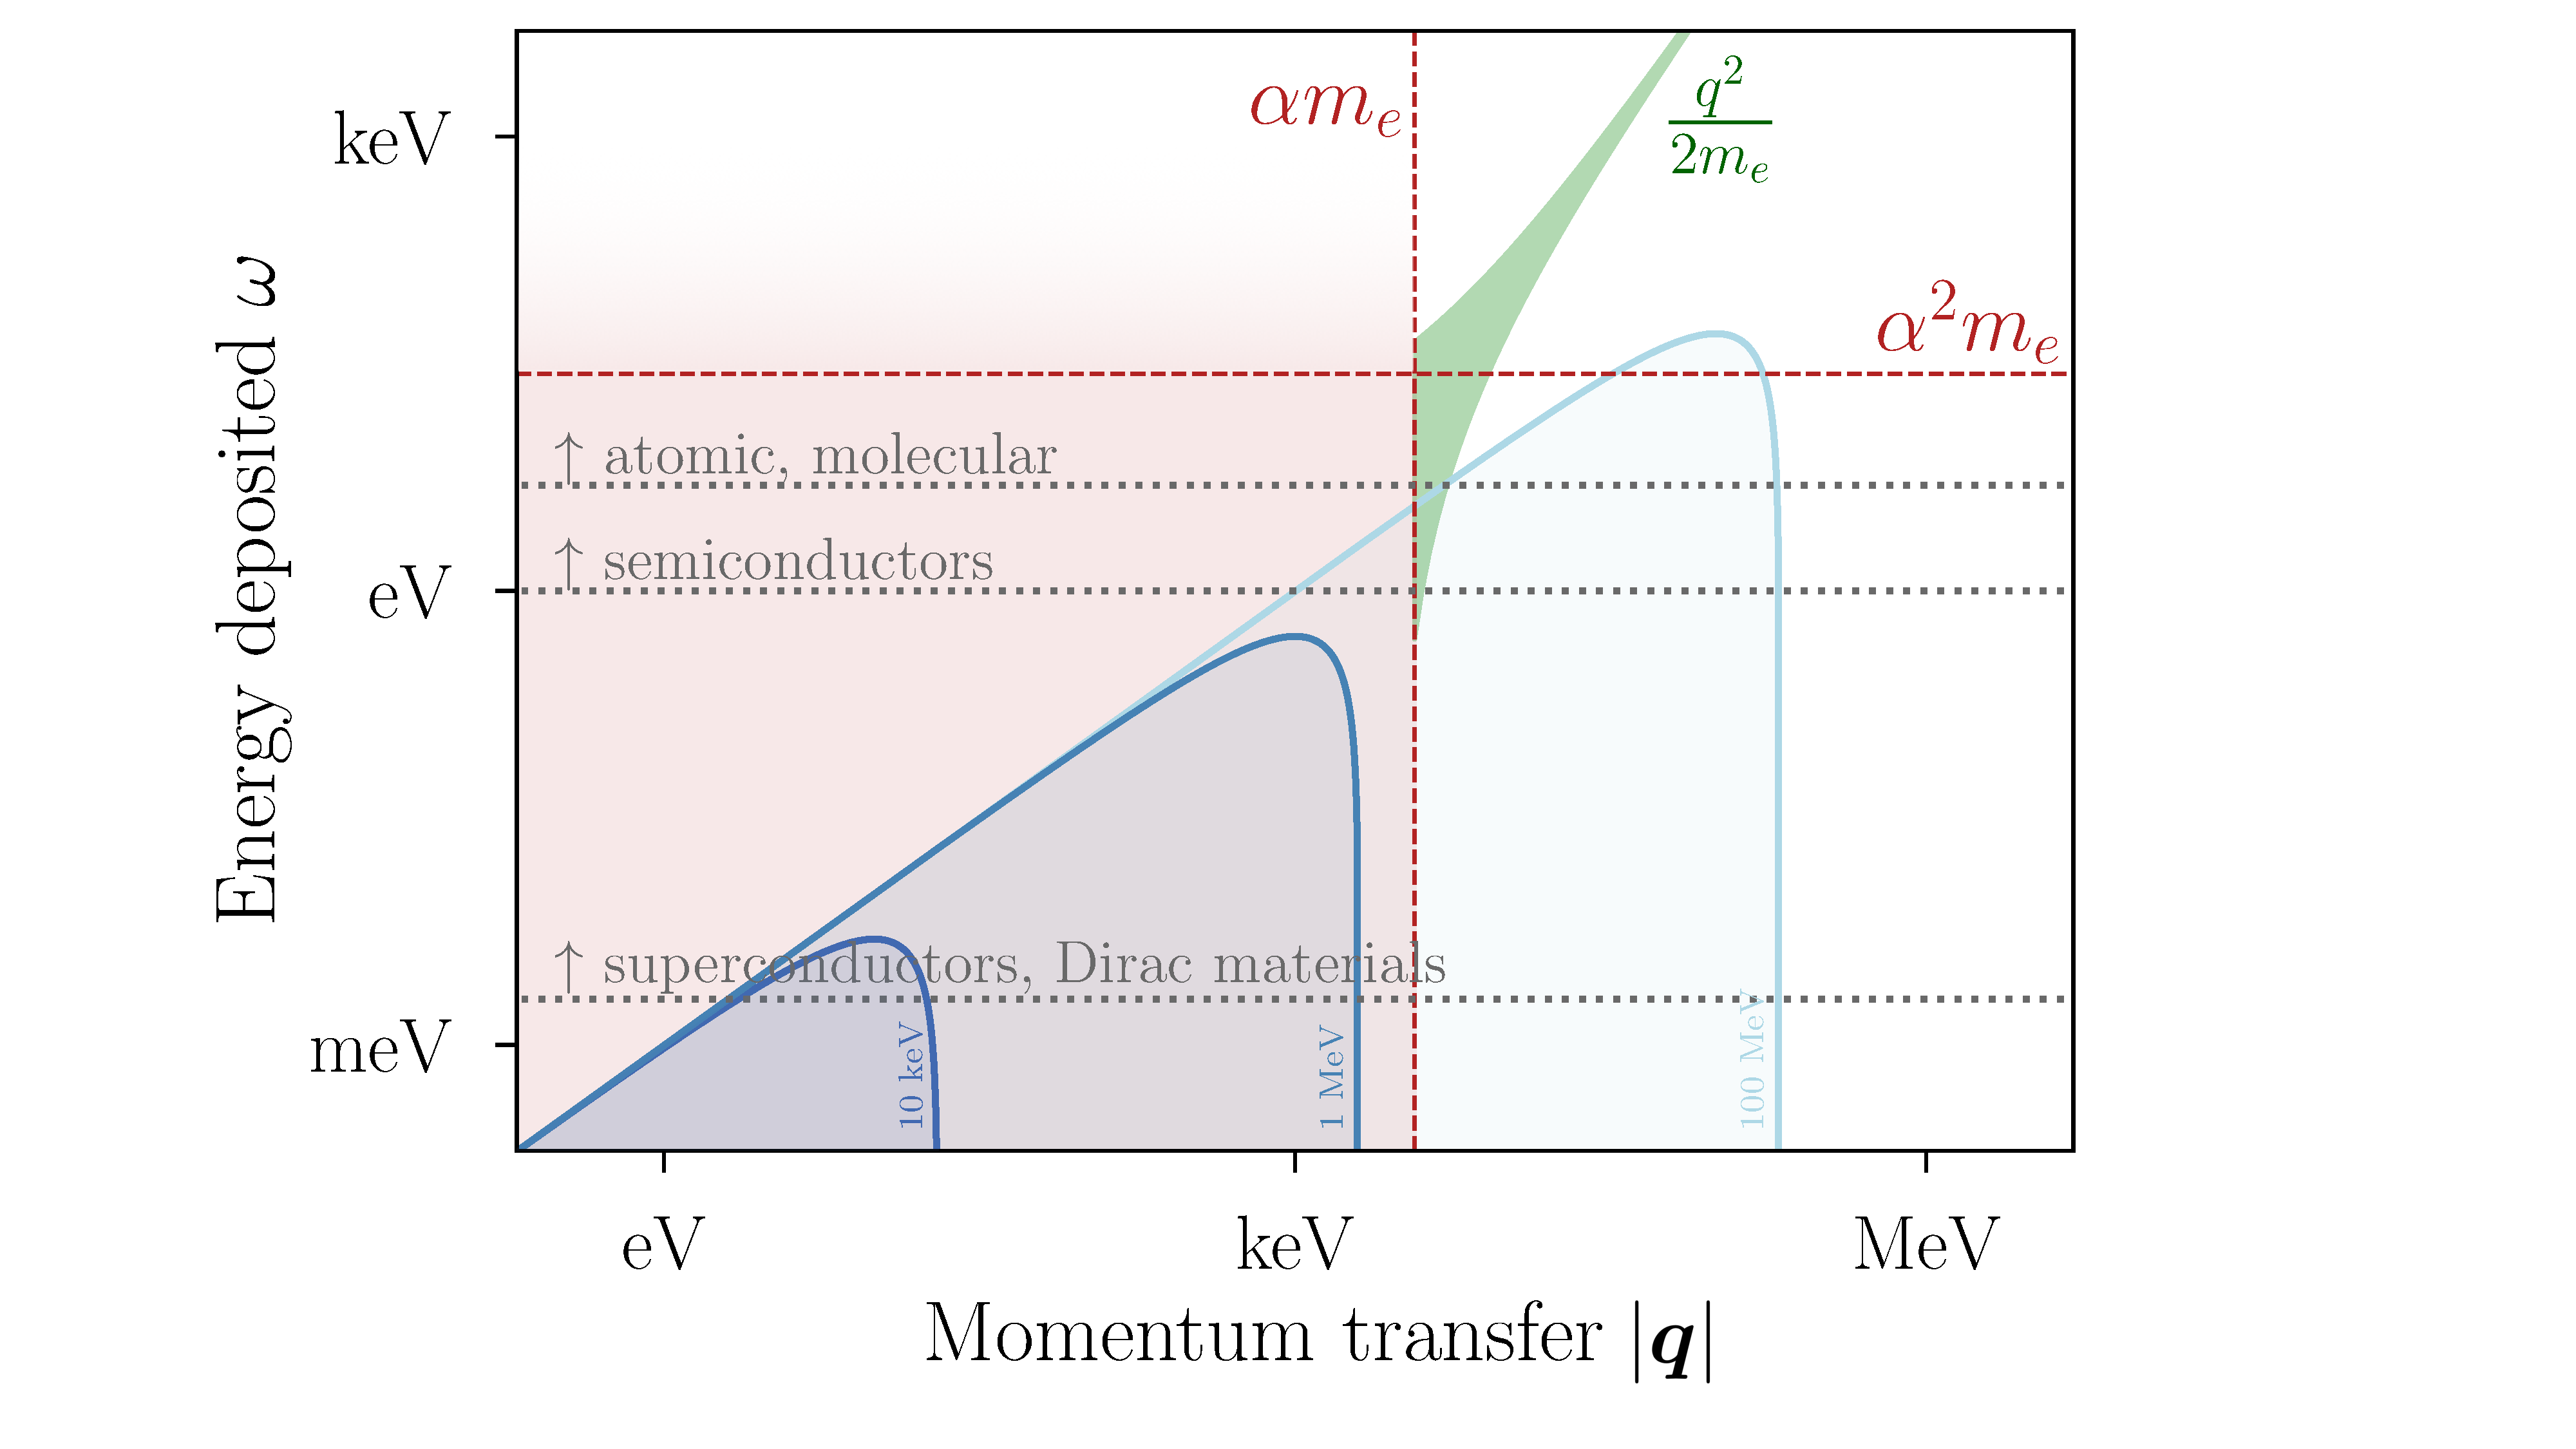
\includegraphics[width=0.45\textwidth]{figs/RPP_massparabolas_electron_gradient}
\qquad
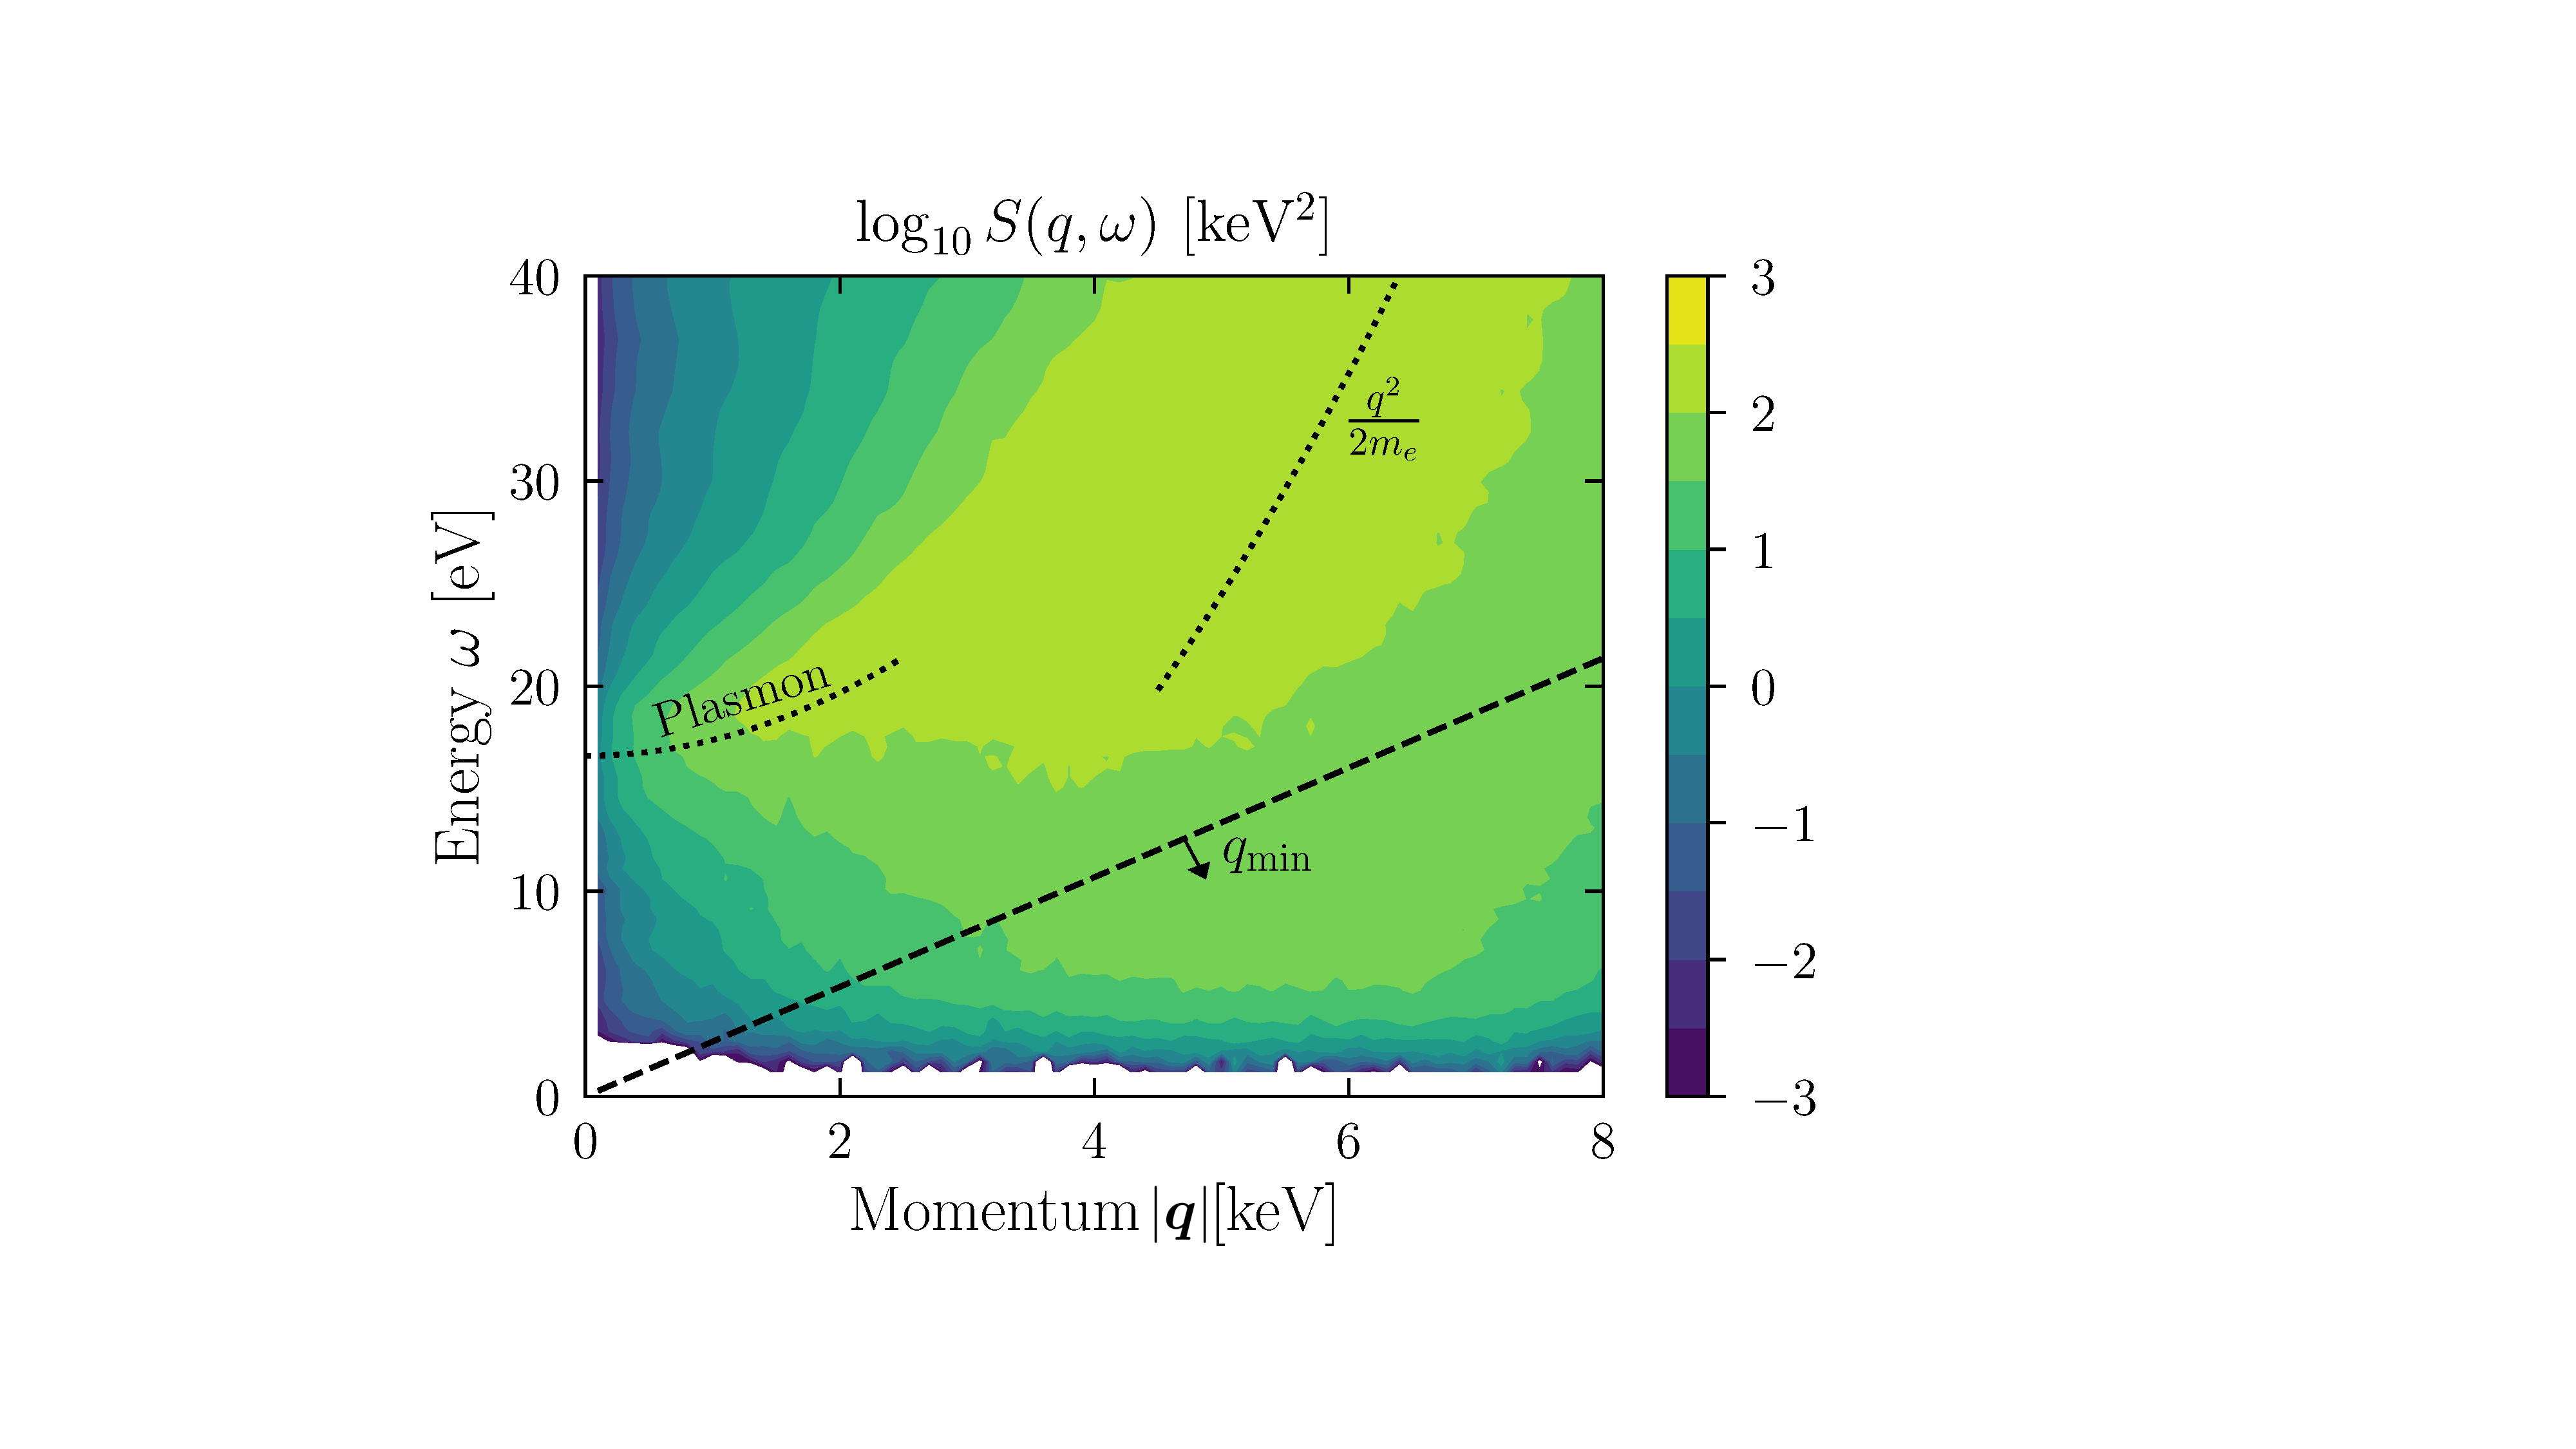
\includegraphics[width=0.48\textwidth]{figs/Si_Sqw}$$
\caption[Direct detection of sub-GeV DM]{\label{fig:DM:electrons}\it {\bfseries Left}: schematical kinematic regions for DM scattering on electrons with $q$ the momentum transfer and $\omega$ the energy deposit. The green band shows the typical response of the material close to the region where the free electron gas approximation becomes reasonable. The blue regions show the kinematically allowed energy deposits, $\omega$, as a function of the momentum exchange, $|\vec q|$, for DM masses $M=10{\rm \,keV}, 1{\rm \,MeV}, 100{\rm \,MeV}$ and initial DM velocity $v=10^{-3}$. The dashed red lines show the typical scale of the wave-function spread ($q\sim 1/a_0=\alpha m_e)$ and the energy ($\alpha^2 m_e)$ of bound electrons. The fact that the electrons are bound inside the material is typically important in the red shaded region. There is a lower bound on the required deposited energy $\omega$ due to energy gaps with typical values for different systems as indicated on the grey dotted lines. For small $\omega$ and $q$ also many body effects can become important.  {\bfseries Right}: the density plot of the dynamical structure factor $S(q,\omega)$ for ${\rm Si}$. From~\cite{dm:light:review} ($\copyright$IOP Publishing, reproduced with permission). 
}
\end{figure}



\smallskip

There is a completely general kinematical limit as to how big the energy deposit $\omega$ in the DM scattering event can be. From energy conservation we have
\beq
\omega(\vec q)=E_1-E_2=\frac{1}{2}M v^2 -\frac{1}{2M}\big(M\vec v -\vec q)^2=\vec q\cdot \vec v -\frac{\vec q^2}{2M}\leq q  v -\frac{ q^2}{2M},
\eeq
so that the deposited energy, $\omega \leq M v^2/2$, lies below a DM mass dependent parabola, shown with blue in fig.~\ref{fig:DM:electrons} (left panel, note that the log scale is used). 
The deposited energy is smaller for lighter DM. 
The kinematically allowed $(\omega,  q)$ region, where the free electron gas approximation can be used, is reached only for $M$ in the GeV regime and above. To have a good sensitivity to DM we want the structure function $S(\vec q, \omega)$ 
to be sizeable in the kinematically allowed region, which means that different materials may be most suitable to be used as targets for various DM masses. In particular, searching for sub-GeV to sub-MeV DM requires materials with small band gaps, as low as meV, such that DM scattering can still cause electronic response, see fig.~\ref{fig:DM:electrons} (left). 
This is sometimes called {\em kinematic matching}. Depositing  energy $\omega$ through DM scattering requires a minimal exchanged momentum
\beq
\label{eq:qmin}
q_{\rm min}=\frac{\omega}{v_{\rm max}}\simeq 3.7\, \text{keV} \biggr(\frac{\omega}{10\,\text{eV}}\biggr)\biggr(\frac{800\,\text{km/s}}{v_{\rm max}}\biggr),
\eeq
where $v_{\rm max}$ is the largest DM velocity in the Earth's frame, $v_{\rm max}\simeq v_\oplus+v_{\rm esc}\simeq 800\,\text{km/s}$, see section~\ref{sec:DMv}. The required momenta exchanges can be large compared to the typical momenta in the condensed matter systems, implying suppressed sensitivity to DM (for an example of such suppression see the discussion following eq. \eqref{eq:f:ion} below). 

\medskip

\subsection{Ionization}\index{Direct detection!ionization}

The ionization energies in atomic systems are controlled by the Rydberg constant, $R_\infty=13.6$ eV, i.e., the ionization energy of hydrogen, and are ${\mathcal O}(10\,\text{eV})$ for the outer shell electrons in noble gases such as xenon and argon, and about ${\mathcal O}(5\,\text{eV})$ for excitation gaps in organic molecules. This means that one can probe DM masses 
from tens of MeV to GeV using such systems as targets, since DM carries enough kinetic energy to ionize the atom or the molecule. However, even in that case there is a suppression associated with the fact that depositing ${\mathcal O}(10\,\text{eV})$ in a system for typical DM velocities requires minimal momentum exchanges that is larger than the inverse size of the bound electron wave functions, $q_{\rm min}> 1/a_0$. The DM scattering cross sections are thus suppressed either by powers of $1/(q_{\rm min} a_0)$, due to suppression of electron wave functions at high momenta~\cite{DM:electron:1203.2531}, 
or require DM from tails of velocity distributions, see eq.~\eqref{eq:qmin}.  
Using eq.~\eqref{eq:S:electron:general} the dynamic structure function for the ionization of atoms is 
\beq
\label{eq:S:ionization}
S(\vec q , \omega) =2 \pi n_{\rm atom} \int \frac{d^3\vec k_e}{(2\pi)^3}\delta( E_f-E_i-\omega) \big|f_{0\to \vec k_e}(\vec q)\big|^2,
\eeq
with $k_e=|\vec k_e|=[2 m_e (\omega -E_B)]^{1/2}$ the momentum of the outgoing electron, $n_{\rm atom}$ the number density of atoms, and $E_B$ the binding energy. The {\em atomic form factor}, $f_{0\to \vec k_e}(\vec q)$, for the electron transition from the ground state to the continuum state with  momentum $\vec k_e$, is given by the weighted overlaps of the initial and final wave functions. For the hydrogen atom it is 
\beq
\label{eq:f:atom}
f_{0\to \vec k_e}(\vec q)=\int d^3\vec r\, \psi_{\vec k_e}^*(\vec r) \psi_{100}(r) e^{i \vec q \cdot \vec r},
\eeq
where $\psi_{100}$ is the  ground state ($n=1,\ell=0, m=0$) wave-function of the hydrogen, and the continuum outgoing state is 
$\psi_{\vec k_e}\propto \exp (- \vec k_e \cdot \vec r)$ for $r\to \infty$. 
For heavier atoms (for instance for noble gas atoms commonly used in direct detection experiments) the two single electron wave functions in eq.~\eqref{eq:f:atom} are replaced by the corresponding multi-electron wave-functions, and $e^{i \vec q \cdot \vec r}\to \sum_i^{N_e} e^{i \vec q \cdot \vec r_i}$, where the sum is over all the electrons in the atom. In the Hartree-Fock approximation the exact many-electron wave functions are approximated by Slater determinants of single-particle wave functions, of $N_e$ bound electrons in the initial state, and of $N_e-1$ bound electrons and one continuum wave function in the final state~\cite{ionization:form:factors}.   


Often we are interested in the spectrum of ionized electrons, i.e., in the differential rate $dR/d E_e$, where $E_e=\omega-E_B$ is the energy of the ionized electron. To obtain $dR/d E_e$ we use a quantity related to the dynamic structure function in eq.~\eqref{eq:S:ionization}, but without evaluating the integral over the magnitude of the electron momentum, $k_e$. It is then convenient to define the {\em ionization form factor}
\beq
\label{eq:f:ion}
\big|f_{\rm ion}( k_e,  q)\big|^2=\sum_{\ell, m} \frac{2  k_e^3}{(2\pi)^3}\big|f_{0\to k_e,\ell,m}(\vec q)|^2,
\eeq
where $f_{0\to  k_e,\ell,m}(\vec q)$ is given by a similar overlap integral as in eq.~\eqref{eq:f:atom}, but now with the outgoing wave function $\psi_{ k_e,\ell,m}(\vec r)$ that describes a spherical wave with a definite angular momentum quantum numbers $\ell, m$. That is, the outgoing wave function $\psi_{\vec k_e}$ is expanded in spherical waves, and thus the integral over $d^3\vec k_e$ in eq.~\eqref{eq:S:ionization} is replaced by a summation over $\ell, m$ and an integral over $d k_e$. This gives
\beq
\frac{dR^{\rm SI}_{\rm ion}}{dE_e}=\frac{1}{E_e}\frac{N_T}{M_T}\frac{\rho_\oplus}{M} \frac{1}{8 \mu_e^2} \int dq \, q \, \bar \sigma(q)  \big|f_{\rm ion}( k_e,  q)\big|^2 \eta(v_{\rm min}),
\eeq
where $\bar \sigma(q)$ is given in eq.~\eqref{eq:sigma:el}, while the minimal DM velocity for obtaining an ionized state with an outgoing electron with energy $E_e$ is given by $v_{\rm min}=\big(E_e+E_B\big)/2 +q/2M$.

The scattering rates for ionization are suppressed by the relatively large exchange momenta compared to the atomic scales. 
Taking as an example the ionization from the ground state of the hydrogen atom in the large momentum exchange regime,  $|\vec q|\gg |\vec k_e| \gg 1/a_0$,  the ionization form factor is proportional to $|f_{\rm ion}|\propto (a_0  k_e)^3/(a_0 q)^8$, showing the parametric suppression from the wave function overlaps. 


\subsection{Semi-conductors} 
Semi-conductors (Si or Ge) are one of the most commonly used materials in direct detection experiments, both because it is relatively easy to produce pure detectors using semi-conductors, as well as because such detectors can potentially detect low mass dark matter, $M<1$ MeV, when scattering on electrons (however, see below for challenges).
The conventional semi-conductors have energy gaps between electronic bands that are ${\mathcal O}(\text{eV})$. This means that in DM scattering events the momentum exchange is always larger than the inverse distance between the atoms in the lattice, see eq.~\eqref{eq:qmin}. The collective effects are thus expected to be less important for DM scattering on conventional semi-conductors. 

Nevertheless, 
the valence electrons are delocalised in a crystal
so that their wave-functions have support throughout the whole crystal, which needs to be taken into account when calculating DM scattering rates. Since we are mostly interested in the spin independent scattering on non-relativistic electrons we can use that the electromagnetic current $\langle e |\gamma^\mu |e\rangle\to (1_{\rm el},\vec 0)$ in the non-relativistic limit. The response of the material to the DM interaction ${\mathcal O}_1^{\rm el}= 1_{\rm DM} 1_{\rm el}$ can therefore be related to the response of the material to the electromagnetic interactions, encoded in the dielectric function $\epsilon(\vec q , \omega)$.  After some algebra one obtains~\cite{Knapen:2021run,cond-mat-book}
\beq
\label{eq:S:ELF}
S(\vec q, \omega)=\frac{\vec q^2}{2\pi \alpha}\Im \biggr(-\frac{1}{\epsilon(\vec q, \omega)}\biggr)\frac{1}{1-\exp(-\omega/k_B T)}.
\eeq
The energy loss function $\Im\big[-1/\epsilon(\vec q,\omega)\big]=\Im\big[\epsilon(\vec q,\omega)\big]/\big|\epsilon(\vec q,\omega)\big|^2$ describes the rate for the charged particle traversing the material to lose momentum $\vec q$ and energy $\omega$. 
Note that $\epsilon$ depends on both $\vec q$ and $\omega$, and thus generalizes the frequency dependent dielectric constant $\epsilon(\omega)$, which describes the response of  a material to the propagating electromagnetic wave (the on-shell photons). 
In scattering of DM, on the other hand, $q\gg\omega$, see fig.~\ref{fig:DM:electrons} (left), so that $\epsilon(\vec q, \omega)$ describes the response of a material to the exchange of off-shell ``potential photons''. 
Sometimes  the screening factor is approximated as $1/\big|\epsilon(\vec q,\omega)\big|^2 \simeq 1$, which is a reasonable approximations for $q\gtrsim $ keV, 
but numerically this still leads to a factor of a few difference in the predicted rates for scattering in Si and Ge. 

Eq.~\eqref{eq:S:ELF} is very useful, since there are both experimental data on the energy loss function as well as established condensed matter techniques to evaluate the structure functions. 
The comparison between different theoretical approaches can then be used to estimate how large the uncertainties are. 
Fig.~\ref{fig:DM:electrons} (right) shows the prediction for dynamical structure function $S(\vec q, \omega)$ for Si, obtained using time dependent density functional theory.  For energy deposits with $\omega \sim 10-20$ eV and low $|\vec q|$  there is a collective excitation --- the plasmon. At higher momenta exchanges the dynamical response function peaks around the free-electron dispersion $\omega =\vec q^2/2 m_e$ with a rather broad support. The region that can be accessed by DM scattering is below the diagonal dashed line, i.e., below the region where collective effects are important. The larger momenta and smaller energy deposits that characterise the DM scattering events therefore  imply suppressed values of $S$. 

\subsection{Novel/low threshold materials} 
\label{sec:novel:material}
DM scattering either on electrons bound in atoms or on electrons inside the semi-conductors is not ideally kinetically matched, with the largest values of $S(\vec q, \omega)$ lying outside the accessible region of momenta and energy exchanges.  
Efforts devoted to finding more suitable target materials with smaller band gaps include the superconductors and Dirac materials, 
see fig.~\ref{fig:DM:electrons} (left). 


Interestingly, superconductors were historically the first materials proposed for detection of dark matter recoils. The idea for the so-called superheated superconducting colloid detectors was that they would consist of superconducting grains of materials cooled just below the transition temperature \cite{DM:nucleon:superconductors}. DM scattering on a nucleus would then deposit enough energy to raise the temperature in the grain and trigger the transition from superconducting to normal phase, resulting in a signal that could be read out. This original detector concept was never used for DM detection, but did motivate searches for DM nuclear recoils using other types of detectors based on semi-conductors and noble gases. The interest in superconductors as possible detector materials has been revived more recently with the increased interest in sub-GeV DM that could be searched for via scattering on electrons \cite{DM:electron:superconductors}, with first bounds now appearing using superconducting nano-wires \cite{DM:electron:superconductors:nanowiresHochberg,Gelmini:2020xir,LAMPOST}. The electrons in a superconductor are bound into Cooper pairs, with typical binding energy in the meV regime. DM scattering on electrons would break Cooper pairs, resulting in a visible signal, potentially even for sub-MeV DM. The practical problem is that the deposited energy needs to be large enough not just to break the Cooper pair but to also pull the electron out from 
the Fermi sea, i.e., to avoid the Pauli blocking. Effectively, this means that the reach of superconducting targets to sub-MeV DM is limited by the screening effects encoded in the behaviour of the dielectric constant at small $q$ \cite{Knapen:2021run}. 


For DM with mass above MeV the conventional semi-conductors based on Ge and Si targets thus still remain the best. For semi-conductors there are no large screening effects in the low wavelength limit, $q\to0$. This is a common feature for all materials that have a Fermi level lying between the valence and conducting bands. The sensitivity to sub-GeV DM is still cut-off, though, by the ${\mathcal O}(1\,\text{eV})$ energy gap between the two bands in the semi-conductors, but could be improved with sensitivity to lower DM masses, if detectors were built from novel narrow-gapped semiconductor materials.
 An example of such a narrow-gap semiconductor is a gapped Dirac material \cite{Vafek_2014}, in which the  conducting and valence bands have a linear dispersion relation, $E_\pm=\pm\sqrt{v_F^2 \vec k^2+\Delta^2}$, the same as the dispersion relation for the relativistic fermions.\footnote{We use the notation in which the energy is measured with respect to the midpoint between the conducting and valence bands, so that the gap is $2\Delta$. The states in the valence band carry negative energies, and correspond to anti-particles in the relativistic theory; $\Delta$ plays the role of the Dirac mass, while Fermi velocity $v_F$ plays the role of the speed of light.} The appearance of the relativistic dispersion relation (in contrast to the non-relativistic one, $E\propto \vec k^2$) in a condensed matter system may seem surprising, since individual electrons are non-relativistic. However, the relativistic dispersion relation  is not a sign of degrees of freedom propagating at the speed of light, but rather a result of being able to Taylor expand 
 the energy levels linearly  in $\vec k$ around special (``Dirac'') point $\vec k_0$ at which the valence and conducting bands touch, if such a point exists. This gives the limit $\Delta \to0$. A small band gap $\Delta \sim {\mathcal O}(\text{meV})$ is obtained, if the lattice symmetry is broken, for instance, by applying strain on a Dirac material. 
The gap is important for practical purposes, since it suppresses thermal noise, a required property for constructing a viable DM detector \cite{DM:electron:Dirac:material}.  Dirac materials also have a useful property: in general $v_F$ is different in different crystal directions, which can then be used to search for DM signal via daily modulation of the signal~\cite{DM:Dirac:amt:directional} (isotropic materials too can measure directionality, if for the scatterings on single quasiparticles the correlation between the direction of the DM wind and outgoing quasiparticle can be traced; an example was worked out for superconductors in \cite{DM:supercon:directional}).  


Some other ideas for DM direct detection are resonant DM absorption in molecules  \cite{1709.05354}, via chemical bond breaking  \cite{1608.02940}, and color centers in crystals \cite{1705.03016}. 
The detection threshold can also be lowered by scattering on collective modes. 
The use of DM scattering on quasiparticles was discussed already in the '80 (for an early review see~\cite{Primack:1988zm}). 
If DM couples to electron spin, this can for instance induce magnon excitations \cite{1905.13744}, 
while low energy DM-nucleon scattering can result in single or few phonon excitations, for instance in polar materials, see the discussion in section~\ref{sec:phonons}.



\subsection{Dark matter absorption}
If DM is a light boson, either a scalar of a vector, with a mass below keV, it can be absorbed in a material resulting in electron excitation \cite{DM:electron:absorptions}. The kinematics of DM absorption is very different from DM scattering, since now we have $\omega=M$ and $\vec q\approx 0$, i.e., $\omega\gg |\vec q|$. For $M\sim {\mathcal O}(10\text{\, eV})$ the absorption of a bosonic DM in a semiconductor can thus excite a plasmon, resulting in an enhanced signal. For instance, if DM is a kinetically mixed dark photon, the absorption rate per unit target mass is given by the energy loss function at (effectively) zero momentum exchange, 
\beq
R=\frac{\rho}{\rho_T}\varepsilon^2\, \Im\biggr[\frac{-1}{\epsilon(0,M)}\biggr],
\eeq
where the parameter $\varepsilon$ gives the strength of kinetic mixing between dark photon and the usual photon, see section~\ref{sec:VectorPortal} (here we use $M$ for DM mass as usual, and not $m_{A'}$). Optical measurements directly probe $\epsilon(0,M)$ and thus one can use data to predict the absorption rate. 


\subsection{Codes for DM electron scattering}
There are several codes that predict DM--electron scattering rates.
{\tt QEdark} uses density functional theory to predict spin independent scattering on electrons in silicon, and is a companion code to the first direct detection limits on sub-GeV dark matter based on recasting the published results from DAMIC~\cite{QEdark}. This was then extended to general DM EFT operators in {\tt QEdark-EFT} (\arxivref{2210.07305}{Catena et al. (2022)}~in \cite{DM:electron:EFT}, for fast parameter scanning there is also a machine learning based speed-up version {\tt DEDD} available, \arxivref{2403.07053}{Catena et al. (2024)}~in \cite{DM:electron:EFT}). 
{\tt DarkELF} \cite{darkELF} performs three different evaluations of the energy loss functions relevant for DM scattering on electrons for a number of targets, as well as the evaluations of the Migdal effect and dark matter phonon/scattering rates. The most sophisticated prediction uses time dependent density functional theory (the GPAW method), the most simplistic is based on approximating the  material with a non-interacting Fermi liquid  (Lindhard method), which is then also generalized to include dissipation and absorption (Mermin method).  {\tt EXCEED-DM} combines density functional theory calculations for states near the band gap and semi-analytic approximations for additional states farther away from the band gap to obtain predictions for DM--electron scattering rates in Si and Ge also for larger energy depositions \cite{Exceed-DM}.  {\tt QCDark} calculates the dark matter-electron scattering rates in crystals using atom-centered gaussian basis, and also estimates systematic uncertainties \cite{QCDark}.  A fast calculation of dark matter direct detection rates in the case of anisotropic materials is provided via the {\tt VSDM} package \cite{VSDM}.


\section{Scattering on phonons}\index{Direct detection!on phonons}
\label{sec:phonons}

The formalism used to include material effects for sub-GeV DM scatterings on electrons 
also applies to scattering of sub-GeV DM on nucleons~\cite{dm:light:review,DM-phonons}. 
For sub-GeV DM the momentum exchange between DM and the material becomes comparable or even smaller than the inverse atomic size, 
and nuclei no longer can be treated as free isolated particles. 
 Depending on the DM mass there are several different regimes of detector response, illustrated in fig.~\ref{fig:DM:phonons}. 
 The red, green and orange shaded regions show the regions where the dynamical structure for spin-independent scattering on nucleons, 
 \beq
 \label{eq:S:nucleon}
 S(\vec q, \omega)=\frac{2\pi}{V} \sum_f \big| \langle f | \sum_I f_I e^{i \vec q \cdot \vec r_I}|i\rangle\big|^2 \delta(E_f-E_i -\omega),
 \eeq
 has large support, and correspond to different physical processes as we discuss below.  In eq.~\eqref{eq:S:nucleon} the sum over $I$ runs over all the nuclei, with  positions $\vec r_I$. In general, the target material is composed of several different atoms, for instance the Na and I for NaI crystals. The $f_I$ are the normalized interaction strengths for DM coupling to nucleon $I$,\footnote{Other normalizations are also used in the literature. For instance, if DM couples to both electrons and nuclei, the dynamical structure function is given by
 \beq
 \label{eq:S:nucleon:electron}
 S(\vec q, \omega)=\frac{2\pi}{V} \sum_f \big| \langle f | \sum_k f_k e^{i \vec q \cdot \vec r_k} + \sum_I  f_I e^{i \vec q \cdot \vec r_I}|i\rangle\big|^2 \delta(E_f-E_i -\omega),
 \eeq
 where $f_k$ is the normalized spin-independent DM coupling to electrons and $f_I$ to nuclei. Conventionally, one often uses $f_e=1$ and $f_I=\big[ Z_I c_1^p/c_1^e + (A_I-Z_I) c_1^n/c_1^e \big]F(q)$. Taking as an example the dark photon, this gives $f_I=-Z_I$ in the long wavelength limit, $q\to 0$. 
}
 \beq
 f_I=\biggr(\frac{ 2}{{|c_1^p|^2+|c_1^n|^2}}\biggr)^{1/2}\Big[ Z c_1^p+ (A -Z) c_1^n\Big]F(q),
 \eeq
 where $c_1^N$ are the non-relativistic coefficients in the effective interaction Lagrangian, eq.~\eqref{eq:LNR}, while $F(q)$ is the spin-independent nuclear form factor, cf. eq. \eqref{eq:dsigmaAdER}.  For isospin symmetric coupling, $c_1^p=c_1^n$, the normalized interaction strength is $f_I=A$ in the $q\to 0$ limit. Both $F(q)$ and $A, Z$ depend on the type of nucleus DM scatters on, so that in general $f_I$ changes from one type of nucleus to another, if DM couples differently to neutrons and protons, $c_1^p\ne c_1^n$.  This means that for DM scattering on nucleons there is, for each of the target materials, not just one but a whole family of dynamical structure functions $S(\vec q, \omega)$, depending on which value the ratio $c_1^p/c_1^n$ takes.
 
\begin{figure}
\center
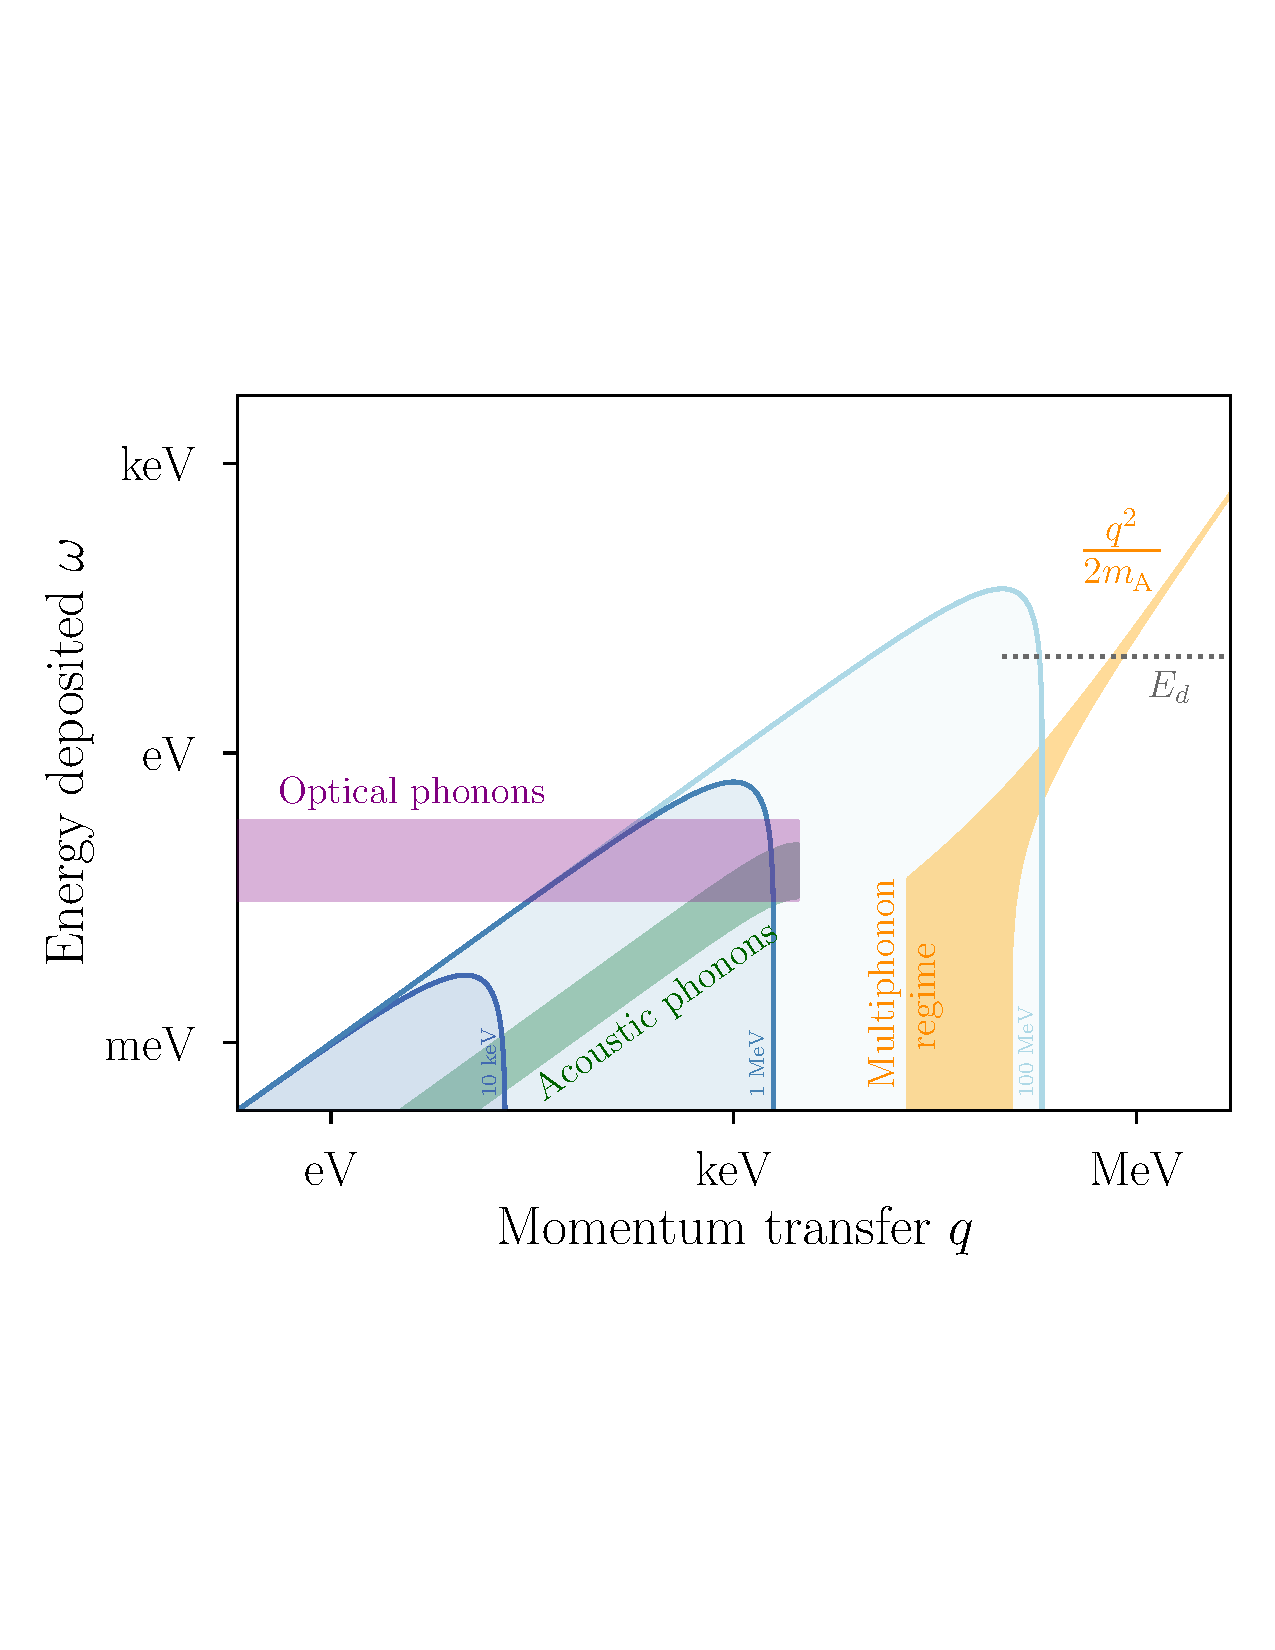
\includegraphics[width=0.55\textwidth]{figs/RPP_massparabolas_nuclear}
\caption[Phonons]{\label{fig:DM:phonons}\it  Different kinematical regions  relevant for DM scattering on nuclei. The free particle regime, $\omega\simeq \vec q^2 /2m_A$,  is approached for large momenta exchanges, and deposited energies well above the  displacement energy for a nucleus, $E_d$. 
Adapted from~\cite{dm:light:review} ($\copyright$IOP Publishing, reproduced with permission).  }
\end{figure}

 
 For heavy DM, $M\gtrsim \GeV$, the energy exchange is bigger than the binding energy and thus the nuclei can be treated as free particles, as done in section \ref{sec:DMscatt:nuclei}. In this case the structure function is given by the free-nucleon limit up to nuclear corrections
 \beq
 \label{eq:S:free:nuclei}
 S(\vec q, \omega)= 2\pi n_{\rm nuc}  A^2 \big|F(q)\big|^2 \delta\Big(\omega -\frac{\vec q^2}{2m_A}\Big),
 \eeq
 where for simplicity we assumed that the DM interaction is isospin symmetric, $c_1^p=c_1^n$. This is shown schematically in fig.~\ref{fig:DM:phonons} as the  orange band. 
 For energy deposits bigger than $E_d\sim {\mathcal O}(10\,\text{eV})$, the typical binding energy of atoms (nuclei) in molecules or condensed matter systems, the structure function approaches the free particle dispersion relation centered at $\omega - \vec q^2/2 m_A$. For DM with masses above $M\gtrsim {\mathcal O}(10\,\text{MeV})$ the binding energy of atomic systems
 becomes important, and needs to be taken into account. 
 The typical momentum exchange $|\vec q|\sim M v \gtrsim {\mathcal O}(10\,\text{keV})$, however, is large enough that the DM scattering can still be viewed as 
 occurring mostly on a single bound nucleon. Viewed as a particle in a potential well, the nucleus behaves as a harmonic oscillator in the ground state. The scattering event excites the harmonic oscillator to a higher energy level, resulting in the spread of the dynamical structure function around the free particle dispersion relation, eventually leading to the multi-phonon regime for small enough momenta transfers. 
 
 \smallskip
 
 For DM with masses below ${\mathcal O}(\text{MeV})$ the maximal momentum transfer is below $\sim 1 $ keV. That is, the de Broglie wavelength of $|\vec q|$ is larger than the interatomic distance in a crystal lattice. For sub-MeV DM one therefore needs to take into account the couplings between different nuclei. DM scatters coherently on collective modes, phonons, which are  the collective vibrational modes of the nuclei arranged in the crystal lattice. The so-called acoustic phonons have a linear dispersion relation $\omega_q=c_s |\vec q|$, where $c_s$ is the speed of sound. Acoustic phonons are massless Goldstone bosons associated with the spontaneous breaking of the translational symmetry. They are given by the oscillational modes that correspond in the $q\to 0$ limit to coherent shifts of all atoms in the same direction. Typically, crystals have more than one atom per unit cell so that other vibrational modes beside acoustic phonons  also exist. 
 The vibrational modes, where atoms within unit cell oscillate with the opposite phase, gives rise to optical phonons, i.e., phonons that are gapped.\footnote{Consider for instance the example where a unit crystal cell has two atoms. If these oscillate around their center of mass system, there is no net momentum flowing in and out of the unit cell, corresponding to a phonon with $\vec q=0$, but with nonzero oscillation frequency (a.k.a. a mass gap). Such an oscillation, but modulated with a long wavelength off-set in the oscillations of the atoms in different cells, then gives an optical phonon with $\vec q\ne0$.}   Optical phonons are thus quasiparticles with nonzero mass $\omega_{\rm optical}\simeq c_s/a \sim {\mathcal O}(10\text{s}\, \text{meV})$, where $a$ is the lattice spacing. The structure functions corresponding to single acoustic and single optical phonon excitations are denoted in fig.~\ref{fig:DM:phonons} as green and magenta bands, respectively.

For detection of DM scattering on phonons, other condensed matter systems, besides crystals, may possibly be used as well~\cite{DM-superfluid-He,DM-polar-materials}. In fact, the use of DM scattering off phonons as a possible detection technique for sub-GeV and sub-MeV DM was first considered for superfluid ${}^4$He (the proposal to use superfluid helium-4 as a DM detector material dates all the way back to 1988, though at that time not with sub-GeV DM in mind) \cite{DM-superfluid-He}. For $M$ above few MeV the typical momentum exchange in DM scattering on superfluid helium is larger than the inverse of a typical distance between the atoms in the supefluid liquid, and the scattering can be viewed as scattering on individual atoms. For lighter masses, however, the collective effects are important, and DM scattering occurs on collective density fluctuations in the superfluid. The difference between semi-conductors and superfluid is that superfluid ${}^4$He is a strongly coupled system, and thus the predictions for the response function $S(\vec q, \omega)$ are much harder to come by. Beside the acoustic phonon contribution, the dispersion curve in superfluid He also contains two other excitations, the maxon and roton. To obtain $S(\vec q, \omega)$ one can try to use directly the data from neutron scattering, or theoretical tools used for strongly-correlated systems, including EFT methods (the latter however only capture the interactions with acoustic phonons). Since the speed of sound  is lower in superfluid helium than in crystals, $c_2\simeq 2.4\cdot 10^2$ m/s, the DM scattering on a single acoustic phonon is not well kinematically matched. In most cases therefore the scattering of DM results in multiphonon excitations.  

Another interesting possibility are polar materials, i.e., materials composed out of constituents that have nonzero dipole moments~\cite{DM-polar-materials}. The gapped optical phonons in polar materials can be thought of as oscillating dipoles, which can thus have sizable couplings to certain types of dark matter, such as the kinetically mixed dark photons. The energy gap for optical phonons ranges from few meV to $\sim100$\,meV, depending on the material. A  useful property of polar materials is that the screening effects are also typically smaller than in superconductors and in Dirac materials. If the crystal is anisotropic, then DM scattering can also result in directional sensitivity. An interesting possibility discussed in the literature are metal halide perovskites, which are being developed in industry for high efficiency photo-voltaics, and could be repurposed for DM searches. 

\section{The Migdal effect}
\index{Direct detection!Migdal}
\label{sec:Migdal}

DM scattering on atoms can result in the  process where DM first scatters on the nucleus, the nucleus recoils, this perturbation gets transferred to the electron cloud surrounding the nucleus, and one of the electrons gets kicked out~\cite{atomic:Migdal}. 
This is the so called Migdal effect: it is a $2\to 3$ inelastic process, with an incoming DM and atom scattering into the final state consisting of an outgoing DM particle, 
an ionized atom and a free electron. This is quite different from the elastic DM/nucleus (DM/atom) scatterings which were the topic of section~\ref{sec:DMscatt:nuclei}. Elastic and inelastic DM/atom scatterings lead to different experimental signatures. 
While elastic DM/atom scatterings result in just the ``nuclear recoils'', the inelastic scatterings result in both the nuclear recoils and  the free electrons (charge deposition) in the detector, more akin to the detector signatures due to DM scatterings on electrons. Since the detector thresholds for detecting electron excitations are typically lower, the Migdal effect can be exploited to extend the sensitivity  of traditional DM detectors to DM/nucleus scattering for lighter DM masses. 

\begin{figure}
\center
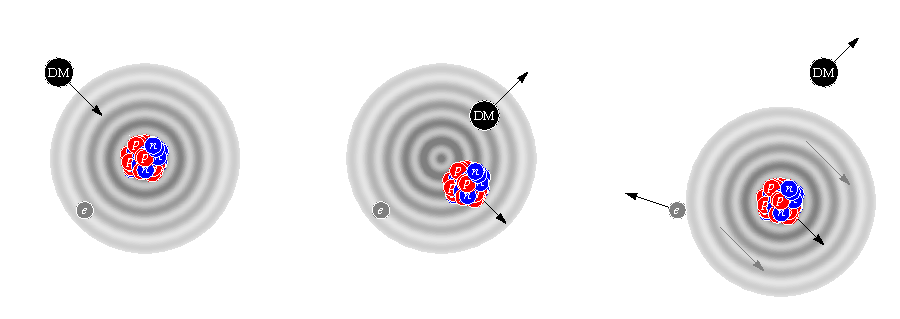
\includegraphics[width=0.9\textwidth]{figs/MigdalIllustration}
\caption[Migdal]{\label{fig:DM:Migdal}\it Illustration of the atomic {\bfseries Migdal effect}, where the scattering of DM on nucleus, and the corresponding nuclear recoil, cause the perturbation of the electronic wave functions, and results in an emission of an electron.  
}
\end{figure}

\smallskip

The structure factor for the Migdal effect, assuming SI DM/nucleus scattering, is
\beq
\label{eq:Migdal}
\frac{d S_{\rm Mig}(\vec q, \omega)}{d\omega_e} \simeq 2\pi n_{\rm nuc} A^2\, 
\delta\biggr(\omega -\frac{\vec q^2}{2 m_A}-\omega_e\biggr) 
\frac{dP}{d\omega_e},
\eeq
where $dP/d\omega_e$ is the probability distribution for the energy $\omega_e$ to be deposited in the electron excitation. In 
eq.~\eqref{eq:Migdal} we assumed for simplicity isospin symmetric DM interactions, and set the nuclear form factor to its long wavelength limit, $F(q\to 0)=1$, since experimentally the Migdal effect is most relevant for sub-GeV DM and thus small momenta exchanges. The expression \eqref{eq:Migdal} can be compared with eq. \eqref{eq:S:free:nuclei}, i.e., the expression for the elastic DM--atom scattering. The factorized form of eq. \eqref{eq:Migdal} assumes that the momentum transfer is dominated by the nuclear recoil, with only a small fraction of the momentum carried by the free electron, which is easily satisfied for present experimental thresholds. 

In the `sudden recoil' approximation, i.e., assuming that the DM/nucleus collision occurs at time-scales much faster than the ones describing the dynamics of the electronic system, the initial electron wave-function can be taken to be unperturbed. The probability distribution $dP/d\omega_e$ is then given by
\beq
\frac{dP}{d \omega_e}=\sum_f\big|\big\langle f\big| \exp\Big(i m_e \vec v_A\cdot \sum_k \vec r_k \Big)\big|i \big\rangle \big|^2 \delta \big(E_f-E_i -\omega_e\big),
\eeq
where $\vec v_A=\vec q/m_A$ is the velocity of the nucleus (and thus the ionized atom) after the recoil, and $\vec r_k$ are the positions of the electrons. 
The exponential phase factor is the net result of the nucleus receiving the kick from DM scattering, and is equivalent  to boosting the initial electron wave-function $|i \rangle$ to the new rest frame of the nucleus.
This simple expression was first obtained as a semi-classical approximation by Migdal in 1939, but can also be derived fully quantum mechanically \cite{Baur:Rossel:1983} (for a quick but somewhat heuristic derivation highlighting the required change of variables see ~\cite{dm:light:review}).
Note that the sum over electron positions is in the exponent of the phase factor, in contrast to the case of DM/electron scattering, eq.~\eqref{eq:S:electron:general}, where the number operator resulted in a sum over phase factors. The final states $\langle f|$ are products of the outgoing free electron wavefunctions and of the ionized atom, with the summation running over all the possibilities.  For sub-GeV DM the recoiled nucleus is slow, $|\vec v_A|\ll 1$. Expanding the phase factors to linear order in $\vec v_A\cdot \vec r_k$ we see that the leading contribution to the Migdal effect is due to the dipole transition matrix elements. These can then be related to the measured photo-absorption cross sections. 



\medskip

For the atomic Migdal effect, the Migdal and electron ionization rates are schematically given by 
\beq
\label{eq:Migdal:ion}
\frac{dR_{\rm Mig}/d\vec q}{d R_{\rm ion}/d\vec q}> Z^2\biggr(\frac{m_e}{m_A}\biggr)^2(\vec q r_{\rm atom})^2,
\eeq
where for simplicity we assumed equal couplings of mediators to protons and electrons. Here $r_{\rm atom}\sim a_0$ is the effective atomic radius. The rate for the Migdal effect is enhanced by $Z^2$, due to coherent scattering on nucleus (for isospin symmetric couplings of the mediator this would be replaced by $A^2$).  
On the other hand, the rate is suppressed by the small electron to nucleus mass ratio, $(m_e/m_A)^2$, 
which negates the $Z^2$ enhancement. 
Because of the $(\vec q r_{\rm atom})^2$ factor the Migdal spectrum is dominated by larger momentum transfers than electron ionisations. Taking all three factors into account we see that the rate for Migdal effect can be comparable or exceed the electron scattering rates for heavy atoms. 

\medskip


The Migdal effect can also occur in crystals, and describes the response of the electron distributions in a crystal due to perturbations  from a single recoiling nucleus, resulting in collective electron excitations or ionisations \cite{crystal:Migdal}. In a crystal, the initial and final states are many body states, with valence electrons delocalised across the crystal. The electromagnetic interactions between the nucleus and a valence electron are screened by the bound inner-shell electrons and by all the other valence electrons in the material. The first effect can be modelled by introducing a $k$-dependent ion charge, $Z_{\rm ion}(k)$, while the second effect can be related to the energy loss function $\Im\big[-1/\epsilon(\vec q,\omega)\big]$ in a similar way as for the DM scattering on electrons, see section~\ref{sec:direct:electrons}. 
The relative ionization vs Migdal rate in crystals is expected to be similar to eq.\eq{Migdal:ion}, valid for atoms.


Rather than triggering the emission of an electron, the DM/nucleus collision can instead result in an emission of a photon~\cite{photon:DM:scattering}. 
While this also provides a possibility to reduce the experimental energy thresholds, the corresponding scattering cross sections are smaller than for the Migdal effect, and thus less useful in practice. 

\medskip


The effect predicted by Migdal has not yet been observed.
It has been searched for experimentally at energies relevant for DM detection in liquid Xenon using neutron scattering.
The outcome was a puzzling null result where a positive signal was expected~\cite{exp:Migdal}. 
There are a few possible interpretations. 
One is that the theoretical calculations are overestimating the rate for the Migdal process, at least in the liquid Xenon used for this search. In that case, the DM constraints relying on this process with this target material (e.g.~{\sc Xenon, PandaX}) would need to be revised. 
Another option is that the physics of the recombination of the free electron and the ionized atom is more efficient than foreseen, and therefore the signal is less prominent than expected.
Or it might be that the magnetic moment of the neutrons, used in the experiment, somehow complicates the physics affecting the Migdal process. In such a case, the DM particle, which possesses negligible electromagnetic interactions, would exhibit the expected Migdal effect.


\section{Non-standard direct-detection signals}
\label{sec:direct:nonstandard}
 
The above discussion of direct detection signatures assumed that DM scatters elastically, 
i.e.,\ that DM does not change during the scattering.
It also assumed that DM couples through a simple mediator to the SM. 
More and more complicated scenarios can be considered.
Below, we discuss a sample of possible deviations from minimality with quite important phenomenological consequences. 


\subsection{Direct detection of inelastic DM}\index{Direct detection!of inelastic DM}\index{DM properties!inelastic}\label{sec:inelasticDM}
\label{sec:inelastic:DM:scattering}
Instead of elastic scattering, $\text{DM}+\text{SM} \to \text{DM}+\text{SM}$, the DM particle could change during the scattering event to a different dark-sector state, $\text{DM}+\text{SM} \to \text{DM}'+\text{SM}$ \cite{inelastic:DM}. 
If the new dark state is lighter, $M'<M$, the direct detection scattering becomes an {\em exothermic} reaction 
that can deposit significantly more energy in the detector than what is possible in elastic scattering, 
 $\mu v^2/2$, where $v\sim 10^{-3}$ is the velocity of the DM particle, and $\mu = Mm/(M+m)$ is the reduced mass of the DM/nucleus system~\cite{exothermic:DM}.  
In the opposite case, $M'>M$, {\em endothermic} reactions arise, so that the direct detection scattering 
can even be kinematically completely forbidden, alleviating the direct detection constraints. 
Kinematic closure happens when $M'- M > \mu v^2/2 \sim {\mathcal O}(100\,\text{keV})$.
In such cases it is possible that the scattering is kinematically allowed on heavier nuclei
and forbidden on light nuclei.\footnote{This property was the original motivation to introduce inelastic DM with 
$ M'-M \sim100\,{\rm keV}$ splitting between the states, 
which for a while lead to a viable explanation of the  {\sc Dama}/{\sc Libra} anomaly discussed in section~\ref{sec:DAMA}.}
 If DM scattering results in an inelastic nuclear transition, ${\rm DM}+A^*\to{\rm DM}'+A$, i.e., if DM up-scatters to the heavier state, while the initial nucleus  $A^*$ transitions to a lower energy level $A$, one can search for mass splittings  of up to $ M'-M \sim \text{MeV}$ 
(though, at present the experiments are sensitive  only to very large scattering cross sections)~\cite{2306.04442}.

Inelastic DM can be realized quite naturally.
Let us consider, for example, a fermionic DM: a Dirac 4-component fermion  
$\Psi=(\psi_L, \bar\psi_R)$ is composed from two 2-component Weyl fermions $\psi_{L,R}$.
In general, it can have a Dirac mass term, $M\bar \Psi \Psi
=M \psi_L \psi_R + \hbox{h.c.}$, 
as well as Majorana mass terms, $ \delta_L \psi_L^2/2 + \delta_R \psi_R^2/2 +\hbox{h.c} $.
In the limit of dominant Dirac mass terms, $M\gg \delta_{L,R}$, this is the so called ``pseudo-Dirac'' DM.
The Majorana terms can naturally be small, since they break a possible global U(1) symmetry, the DM number.
The Majorana terms, even if small, qualitatively change the mass eigenstates, which are then
 two quasi-degenerate  Majorana fermions.   In a 2-component notation they are given by
\begin{align}
\chi_1\simeq& i \frac{\psi_L - \bar\psi_R}{\sqrt2}, \qquad m_1\simeq M-(\delta_L+ \delta_R)/2,
\\
\chi_2\simeq& \phantom{i}\frac{\psi_L +\bar\psi_R}{\sqrt2}, \qquad m_2\simeq M+(\delta_L+\delta_R)/2.
\end{align}
In energetic enough scatterings, such that the energy transfer is well above $\delta_{L,R}$,
the splitting can be neglected, and the two states behave as part of a single Dirac fermion.
In the opposite, low-energy limit, the two states behave as two separate Majorana fermions. 

The low energy limit also reveals a  qualitative change in the structure of the interaction.
Assuming a vector current interaction to quarks, $(\bar \Psi \gamma_\mu \Psi)(\bar q\gamma^\mu q)$, 
this corresponds to effectively elastic scattering at high energies (when mass eigenstates are degenerate to a good approximation), but to an inelastic interaction among mass eigenstates at low energies, transforming $\chi_1$ to $\chi_2$ in the scattering:
\beq
\bar \Psi\gamma_\mu \Psi\simeq i \big(\bar\chi_1 \bar \sigma_\mu \chi_2- \bar\chi_2 \bar \sigma_\mu \chi_1\big).
\eeq
A similar phenomenon happens, if a small mass term splits a complex scalar into two real scalars.






\subsection{Baryonic DM and nucleon decay}
Models of baryogenesis  involving dark sectors (section~\ref{sec:AsymmetricDMth}) involve
asymmetric DM carrying anti-baryonic global number, so that the net baryon number, combining visible and dark sectors, is zero.
Antibaryonic DM  can, in a very special case, lead to a spectacular signature in direct detection experiments --- a DM-induced nucleon decay \cite{baryon:decay:asym:DM}. 
If the dark sector consists of two stable states, the anti-baryonic DM and a slightly lighter DM$'$ with no baryon number, 
then the DM can scatter inelastically in the target material, $\text{DM}+p\to \text{DM}'+\pi^+$ or $\text{DM}+n\to \text{DM}'+\pi^0$.
Other mesonic final states with more pions or with kaons, are also possible;
DM with baryonic number $1/3$ can induce $\overline{\text{DM}}+n\to \text{DM}+\text{DM}$.
In all these cases, from observer's point of view, the proton $p$ or a neutron $n$ bound inside a nucleus would appear to decay, a signature usually associated with Grand Unified Theories.  The bounds on such processes are comparable to the bounds on the proton decay itself, and correspond to effective nucleon lifetimes of $10^{29-32}$ years. Note that the mass difference between DM and DM$'$ cannot be too large 
since then decays $\text{DM}\to \text{DM}'+\bar n$ become kinematically open and DM is no longer stable.



\subsection{Secluded DM}\index{Direct detection!of secluded DM}
Secluded DM is a generic mechanism by which direct detection scattering cross sections can be suppressed, while DM is still a thermal relic, however, largely decoupled from the SM \cite{secluded:DM}. Secluded DM does not couple directly to DM, but rather interacts with some extra mediator particles, 
which then couple to the SM. 
In the early Universe the DM relic abundance is determined by annihilations to mediators, i.e., the mediators are lighter than the DM. 
The mediators then decay to SM particles, with couplings that can be very small --- 
lifetimes as long as a fraction of a second are fine, since the mediators still decay before the BBN. 
Since the couplings of mediators to the SM can be very small, this gives highly suppressed direct detection signals, 
possibly well below any present or future sensitivities. 



\begin{figure}[t]
\begin{center}
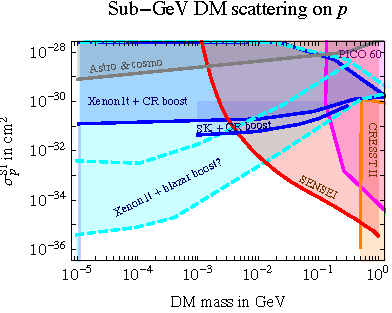
\includegraphics[width=0.45\textwidth]{figs/DirectDetectionSubGeVDMp} \qquad
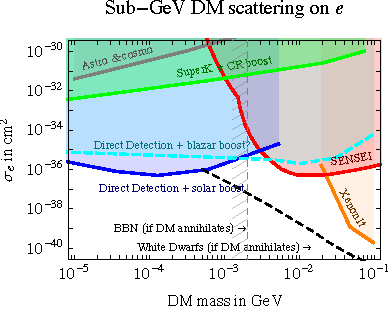
\includegraphics[width=0.45\textwidth]{figs/DirectDetectionSubGeVDMe} 
\end{center}
\caption[Bounds on sub-GeV DM]{\em {\bfseries Bounds on sub-GeV} Dark Matter. 
Boosted DM is discussed in section~\ref{BoostedDM}; BBN bounds in~\ref{sec:BBNconstraints};
White Dwarf bounds in~\ref{sec:CaptureWD}. The astrophysical and cosmological bound is taken from \arxivref{2107.12377}{Buen-Abad et al.~(2022)} \cite{SIMP}, see section \ref{sec:SIMP}.
\label{fig:DirectDetectionSubGeVDM}}
\end{figure}



\subsection{Boosted DM}\label{BoostedDM}\index{Direct detection!of boosted DM}\index{DM properties!boosted}\index{Boosted DM}
DM gravitationally bound inside the galactic halo is non-relativistic, 
with velocity below the escape velocity $v_{\rm esc}\approx 10^{-3}$, see section~\ref{sec:DMv}. 
Different processes can accelerate a small fraction of DM particles to higher energies, generating a `boosted DM' component.
Some of the main possibilities are:
\begin{enumerate}
\item Multiple scatterings with fast moving nuclei or electrons inside the Sun, where DM gains kinetic energy and evaporates (the so called {\em solar reflection}). The energy transfer is large enough that sub-GeV DM can now have enough energy to be seen in direct detection experiments ~\cite{CR:DM:Sun}.
\item Collisions of DM particles with cosmic rays in the Galactic environment; 
this boosted component of the DM wind is sometimes called the {\em cosmic ray DM}~\cite{CR:DM:CR}.
\item A similar effect could arise around sources of cosmic rays, especially blazars such as the BL Lacert\ae{}
(the nearby active galactic nucleus that emits a jet pointing towards us). 
The resulting flux of boosted DM depends on the uncertain DM density around such sources~\cite{CR:DM:blazars}.
\item The evaporation of Primordial Black Holes at present times \cite{Boosted:PBH:DM}. This is analogous to the process that could have produced DM particles in the early Universe~\cite{DMfromPBH}. PBHs with masses from $10^{14}$ to $10^{16}$ g are a source of boosted MeV DM with energies of tens of MeV.
\item Decays or annihilations of heavier dark matter states;
this possibility is, however, more speculative and model dependent~\cite{Boosted:DM}. 
\end{enumerate}
Boosted DM is an especially important effect for sub-GeV DM. After boosting, the DM particle can have enough kinetic energy to give
a detectable energy deposition in direct detection targets,  above the experimental threshold.
By taking into account this effect, the lower reach of DM direct detection experiments 
gets extended down to $M\approx 100 \ \text{keV}$ DM masses~\cite{Boosted:DM:exp},
as illustrated in fig.\fig{DirectDetectionSubGeVDM}.
We also mention that, as a related application, \arxivref{2307.09460}{Herrera and Murase (2023)  \cite{CR:DM:CR}} derived constraints on sub-GeV DM scatterings on protons and electrons via the requirement that cosmic rays emitted by AGN are not slowed down too much by the interactions with the surrounding DM.



\subsection{Self-destructing DM}\index{Direct detection!of self-destructing DM}
A long lived DM state might convert through scattering on nucleus or electron into a short-lived dark sector state \cite{Self:destr:DM}. 
This then decays to standard model particles within the detector, giving a visible deposited energy  that can be comparable to DM mass --- 
many orders of magnitude larger than the recoil energy deposited during elastic scatterings. 
This allows to search for self-destructing DM in large detectors with high energy thresholds, 
such as the neutrino detectors and not just with dark matter direct detection experiments. 




\subsection{Absorption of DM}\index{Direct detection!absorption}
If DM has interactions with the SM that involve only a single DM field, such as ${\rm DM}\,\bar q q$ or ${\rm DM}\,\bar e e$, 
then the DM particle can get absorbed in the target material when interacting with an electron or with a nucleon \cite{absorption:DM}. 
Such interactions also induce DM decays and therefore need to be highly suppressed so that DM is long-lived enough on cosmological time scales. 
This means that absorption of DM is a very rare event. The experimental signature, on the other hand, is quite different compared to DM scattering. 
In DM absorption the deposited energy is controlled by the DM mass, $M$, and is thus six orders of magnitude larger than the  energy 
deposited in the scattering event (controlled by DM kinetic energy, $ M v^2/2\approx 10^{-6} M$). 
Through DM absorption on electrons one can thus probe also very light bosonic DM, with masses in the ${\mathcal O}(10\,\text{eV})$ range 
(see the more detailed discussion in section~\ref{sec:novel:material}).
Absorption is also possible for fermionic DM, by emitting a light SM fermion in the process (similarly to interactions of SM neutrinos).
Typically, the emitted particle is a neutrino, if absorption  is through a neutral current interaction, or an electron, for a charged current interaction. 



\subsection{Multiple scatterings}
The bounds on scattering cross sections of ultra-heavy DM, with mass above $M\gtrsim 10\,$TeV, 
are weak enough to allow events where DM scatters multiple times inside the detector \cite{ultraheavy:DM:direct} 
(the cross section has to be small enough that DM particles reach the underground detector, see also section~\ref{sec:SIMP}). 
Such very heavy DM loses little energy in the scattering event and would travel through the detector in a straight line, leaving behind a track of small energy deposits. Such a signature is distinct enough that it can be distinguished from backgrounds. 
Dedicated analyses of data in conventional direct detection experiments are being performed to search for such events.  


\subsection{Scattering of composite DM}
\index{Composite DM!direct detection}\index{Direct detection!of composite DM}
If DM is a composite object rather than a point-like particle,
this can be accounted for through a DM form factor, $F_{\rm DM}(q)$. In section~\ref{sec:SI} we took  into account nuclear structure in the same way through the use of nuclear form factors. That is, the SI scattering cross section in eq.~\eqref{eq:dsigmaAdER} now gets multiplied by  $F_{\rm DM}(q)^2$ (for SD scattering of composite DM one needs to introduce several form factors, the same as for nuclei in section~\ref{sec:SD}). 
The DM form factor encodes the parametric suppression of scatterings in which momenta exchanges are large compared to the DM size, $r_{\rm DM}$, $F_{\rm DM}(q)\propto \exp(-q^2 r_{\rm DM}^2/2) /(qr_{\rm DM})^2$ for $q r_{\rm DM}\gg 1$, 
see the expression for Helm nuclear form factor below eq.~\eqref{eq:ERmax}. 
Larger $r_{\rm DM}$ implies loosely bound composite DM, in which case there is little momentum and energy transfer between DM and the target in the detector (imagine a ball of very soft foam scattering on a small hard target). 
The bounds from the usual direct detection experiments then become weaker. 
In an extreme situation, thousands or more DM particles can be bound in nuggets, 
held together by a Yukawa potential due to a light scalar mediator. 
Ref. \cite{nugget:levitate} searched for such TeV mass nuggets, for mediators lighter than an eV, i.e., for Yukawa potentials with a range larger than about a $\mu$m. As a sensitive sensor they used an optically levitated sphere, and set bounds on DM-neutron scattering at the level of $\sigma_{\chi n}\lesssim 10^{-26}$\,cm${}^2$ for nugget masses in the TeV range.


\subsection{DM gravitational effects} 
\label{gravisignal}\index{Direct detection!gravitational}\index{Gravitational DM}
DM with a Planck-scale mass that only interacts through the gravitational force can be searched for in the laboratory using an array of mechanical sensors, operated as a single detector. 
The passage of a DM particle with galactic velocity $v \sim 10^{-3}$
through the detector can potentially be measured, if DM is heavy enough, since DM exerts a gravitational force
transferring the impulse
\beq  
p_\perp= \int dt\, F_\perp = \tau \frac{G M m_{\rm detector}}{b^2} \approx 10^{-20}\,\frac{\rm m}{\rm s}\, m_{\rm detector} \left(\frac{{\rm mm}}{b}\right)^2,
\eeq
where $\tau = 2b/v $ is the event duration and $b$ the impact parameter.
This can be compared to the thermal fluctuation $\med{ \delta p_\perp^2} \sim m_{\rm detector} T \tau/\tau_{\rm detector}$
for a single suspended detector  with a mechanical damping time $\tau_{\rm detector} \sim 10^8\,{\rm s}$.
The DM flux is large enough, if DM is light enough,
$\Phi_{\rm DM}= \rho_{\rm DM} v/M\approx 1/({\rm yr}\, {\rm  m}^2)  (M_{\rm Pl}/M)$. This means that
DM with a Planck-scale mass requires detectors with a cross sectional size of about a square meter.
To obtain a measurably large signal will require about $10^6$ gram-size accelerometers. 
A development of such a sensor was proposed by the {\sc Windchime} collaboration~\cite{gravitational:DM:direct}.  
The same type of detectors could search for DM with speculative extra long-range forces.

\begin{table}
\setlength\tabcolsep{1pt} \renewcommand{\arraystretch}{0.95}
\resizebox{\columnwidth}{!}{
\begin{tabular}{llccccc}
\hline
\hline
 {\bf Experiment} & {\bf Location} & {\bf Data taking} & {\bf Readout} &{\bf Target} & {\bf Home} & {\bf Ref.}   \\

\hline
{\sc PNL/USC} & Homestake, SD & 1986 $\to$ 1991 &  ioniz. ($\sim$77\,K) &  $0.7\to2$\,kg Ge & \href{https://dx.doi.org/10.1016/0370-2693(87)91581-4}{paper} & \cite{Ahlen:1987mn} \\

\multirow{2}{*}{{\sc UCSB/LBL/UCB}} & \multirow{2}{*}{Oroville dam, CA  $\biggr\{$} & 1986 $\to$ 1990 &  ioniz. ($\sim$77\,K) &  $0.9\,$kg Ge & \multirow{2}{*}{\href{https://doi.org/10.1103/PhysRevLett.61.510}{paper}} &\multirow{2}{*}{ \cite{Caldwell:1988su}} \\

&  & 1989 &  ioniz. (77\,K) &  17\,g Si&  &  \\

{\sc Gotthard Ge} & Gotthard, Switzer. & 1986 $\to$ 1990 &  ioniz. ($\sim$77\,K) &  0.7\,kg Ge & \href{http://www.nu.to.infn.it/exp/all/gotthard/}{web} & \cite{Treichel:1989cj}
\\


{\sc COSME} & Canfranc, Spain & 1990 $\to$ 1999 & ioniz. ($\sim$77\,K) &  234\,g Ge& \href{https://arxiv.org/pdf/hep-ex/0101037.pdf}{paper} & \cite{Garcia:1995ez}
\\

{\sc Heidel.-Moscow} & Gran Sasso, Italy & 1990 $\to$ 1998 & ioniz. ($\sim$77\,K) & $2.76$\,kg Ge& \href{http://www.klapdor-k.de/Theory\%20of\%20Experiments/HDMDBD/HeiMos.htm}{web} & \cite{Beck:1993sb}
\\

{\sc EDELWEISS-0} & Modane, France & 1991 $\to$ 1994 &  ther. phon. (50\,mK) &  $24$\,g Al${}_2$O${}_3$ & \href{https://doi.org/10.1016/S0927-6505(96)00040-0}{paper} & \cite{Edelweiss-0}
\\

{\sc TWIN} & Homestake, SD & 1992 & ioniz. ($\sim$77\,K) &  $\sim$2.1\,kg Ge& \href{https://doi.org/10.1016/0920-5632(93)90160-8}{paper} & \cite{TWIN}
\\

{\sc BRS} & Gran Sasso/Modane & 1992 & scint. ($\sim$300\,K)  &  0.7\,kg NaI(Tl) & \href{https://doi.org/10.1016/0370-2693(92)91575-T}{paper} & \cite{BRS}
\\

{\sc NaI32} & Canfranc, Spain & 1992 $\to$ 1995 & scint. ($\sim$300\,K)   &  32\,kg NaI(Tl) & \href{https://doi.org/10.1016/0920-5632(96)00211-3}{paper} & \cite{Sarsa:1995yb}
\\

\multirow{2}{*}{{\sc ELEGANT V $\Big\{$}} & Kamioka, Japan & 1992 $\to$ 1998 & \multirow{2}{*}{scint. ($\sim$300\,K)}  &  36.5 $\to$ 662\,kg NaI(Tl) & \multirow{2}{*}{\href{https://doi.org/10.1016/S0927-6505(99)00086-9}{paper}} & \multirow{2}{*}{\cite{ELEGANTV}}
\\

 & Oto-Cosmo, Japan & 1999 $\to$ 2000 &   &  730\,kg NaI(Tl) &  & 
\\

\multirow{2}{*}{{\sc BPRS}~~~~~~$\Big\{$} & Gran Sasso, Italy & 1993 $\to$ 1994 & scint. ($\sim$300\,K)  &  7\,kg NaI(Tl) & \multirow{2}{*}{\href{https://www.sciencedirect.com/science/article/abs/pii/092056329500470T}{paper} }& \multirow{2}{*}{\cite{BPRS}}
\\

 & Gran Sasso/Modane & 1993 & scint. ($\sim$300\,K)  &  0.37\,kg CaF${}_2$(Eu) & & 
\\

{\sc DEMOS} & Sierra Grande, Argen. & 1994 $\to$ 1997 & ioniz. ($\sim$77\,K)   &  $\sim1\,$kg Ge & \href{https://doi.org/10.1016/S0927-6505(98)00047-4}{paper} & \cite{DEMOS}
\\

{\sc UKDM-NaI} & Boulby, UK & 1994 $\to$ 1997 & scint. ($\sim$300\,K)  &  $1.3\to6.2$\,kg NaI(Tl) & \href{https://doi.org/10.1016/0370-2693(96)00350-4}{paper} & \cite{UKDMC-NaI}
\\

{\sc MIBETA} & Gran Sasso, Italy & 1995 $\to$ 2000 &  ther. phon. (10\,mK) &  $0.34$\,kg TeO${}_2$ & \href{http://www.nu.to.infn.it/exp/all/mibeta/}{web} & \cite{MIBETA}
\\

{\sc DAMA/LXe} & Gran Sasso, Italy & 1995 $\to$ 2001 & scint. (170\,K)  &  6.5\,kg LXe & \href{https://dama.web.roma2.infn.it/?page_id=84}{web} & \cite{DAMA-Xe}
\\

{\sc HDMS} & Gran Sasso, Italy & 1996 $\to$ 2003 & ioniz. ($\sim$77\,K) & $0.2$\,kg Ge & \href{http://www.klapdor-k.de/Theory\%20of\%20Experiments/DarkMatter/Recent\%20Results.htm}{web} & \cite{HDMS}
\\

{\sc DAMA} & Gran Sasso, Italy & 1996 $\to$ 2002 & scint. ($\sim$300\,K)  &  $\sim100\,$kg NaI(Tl) &  \href{http://people.roma2.infn.it/~dama/web/ind_nai.html}{web} & \cite{DAMA}
\\

\multirow{2}{*}{{\sc CDMS-I}} & \multirow{2}{*}{Stanford, CA \hspace{4mm} $\Big\{$} & 1996 $\to$ 1999 & ther. phon.+ioniz. (20\,mK)   &  $0.5\to1$\,kg Ge& \multirow{2}{*}{\href{https://www.slac.stanford.edu/exp/cdms/}{web}}&  \multirow{2}{*}{\cite{CDMS-I}}
\\
   & & 1996 $\to$ 1999 & ath. phon.+ioniz. (20\,mK)  &  $0.1\to0.2$\,kg Si&  &
\\

{\sc EDELWEISS-I} & Modane, France & 1997 $\to$ 2004 &  ther. phon.+ioniz. ($\sim20\,$mK) & $70\,\text{g}\to1$\,kg Ge & \href{http://edelweiss.in2p3.fr/index.php}{web} & \cite{Edelweiss-I} 
\\


{\sc Saclay-NaI} & Modane, France & 1997 & scint. ($\sim$300\,K)  &  10\,kg NaI(Tl) & \href{https://doi.org/10.1016/S0927-6505(99)00004-3}{paper} & \cite{SaclayNaI}
\\

{\sc ELEGANT-VI} & Oto Cosmo, Japan & 1998 $\to$ 2007 & scint. ($\sim$300\,K) &  10\,kg CaF$_2$(Eu) & \href{https://doi.org/10.1088/1742-6596/120/4/042019}{paper} & \cite{ELEGANT-VI}
\\

{\sc IGEX-DM} & Canfranc, Spain & 1999 $\to$ 2002 &  ioniz. ($\sim77\,$K) & 2.0\,kg Ge& \href{https://doi.org/10.1016/S0920-5632(03)01401-4}{paper} & \cite{IGEX-DM} \\

\multirow{3}{*}{{\sc ROSEBUD}} & \multirow{3}{*}{Canfranc, Spain $\Biggr\{$} & 1999 $\to$ 2002 & ther. phon. (20\,mK) &  50\,g Al${}_2$O${}_3$& \multirow{3}{*}{\href{https://lsc-canfranc.es/wp-content/uploads/2018/10/ROSEBUD_EN.pdf}{paper}} & \multirow{3}{*}{\cite{ROSEBUD}} \\

 &  & 1999 $\to$ 2002 & ther. phon.+scint.  (20\,mK)  &  $ 54$\,g  CaWO${}_4$ &  &  \\
 
  &  & 1999 $\to$ 2002 & ther. phon. (20\,mK)   &  $ 67\,\text{g}$  Ge &  &  \\

{\sc SIMPLE} & LSBB, France & 1999 $\to$ 2010 &  superheat. dropl. ($\sim$290\,K)  & $15\to215\,$g C${}_2$CIF${}_5$ & \href{https://doi.org/10.1103/PhysRevD.89.072013}{paper} & \cite{SIMPLE}
\\

{\sc CRESST-I} & Gran Sasso, Italy & 2000 & ther. phon. (15\,mK)   &  $262$\,g Al${}_2$O${}_3$ & \href{https://doi.org/10.1016/S0927-6505(02)00111-1}{paper} & \cite{CRESST-I}
\\

{\sc NAIAD} & Boulby, UK & 2000 $\to$ 2003 &   scint. ($\sim 280$\,K) & $46\to55$\,kg NaI(Tl) & \href{https://doi.org/10.1016/S0927-6505(03)00115-4}{paper} & \cite{NAIAD} \\

\multirow{3}{*}{{\sc Tokyo-DM}} & \multirow{3}{*}{Kamioka, Japan $\Biggr\{$} & 2001 $\to$ 2002 &  ther. phon. (10\,mK)  & 168\,g LiF & \multirow{3}{*}{\href{https://doi.org/10.1016/j.physletb.2005.12.025}{paper}}& \multirow{3}{*}{\cite{Tokyo-DM}} 
\\

 & & 2002 $\to$ 2003 &  ther. phon. (4\,K)  & 176\,g NaF &   &  
\\

 & & 2005 &  scint. ($\sim300$\,K)  & 310\,g CaF${}_2$(Eu) &   &  
\\

{\sc ZEPLIN-I} & Boulby, UK & 2001 $\to$ 2003 &  scint. ($\sim 170$\,K) & 3.2\,kg Xe & \href{https://hepwww.pp.rl.ac.uk/groups/ukdmc/project/ZEPLIN-I/zeplin-i.html}{web} & \cite{ZEPLIN-I} \\

\multirow{4}{*}{{\sc CDMS II}~~~$\Biggr\{$} & \multirow{2}{*}{Stanford, CA } & \multirow{2}{*}{2001 $\to$ 2002 } & \multirow{2}{*}{ath. phon.+ioniz. (20\,mK)$\Big\{$}& $1\,$kg Ge & \multirow{4}{*}{\href{https://www.slac.stanford.edu/exp/cdms/}{web}} & \multirow{4}{*}{\cite{CDMS-II}} 
\\
 &  &  &  & $0.2\,$kg Si &  & 
\\
 
 & \multirow{2}{*}{Soudan, MN} & \multirow{2}{*}{2003 $\to$ 2008 } &  \multirow{2}{*}{ath. phon.+ioniz. (50\,mK)$\Big\{$} & $1\to4.6\,$kg  Ge &  &  
\\
 &  &  &  & $0.2\to1.2\,$kg Si &  & 
\\
 
{\sc ORPHEUS} & Bern, Switzerland & 2002 $\to$ 2003 & superheat. grains ($\sim$100\,mK) & 0.45\,kg Sn & \href{https://doi.org/10.1016/j.astropartphys.2004.06.005}{paper} & \cite{ORPHEUS}
\\

{\sc KIMS} & Yangyang, S. Korea & 2004 $\to$ 2012 &  scint. ($\sim300\,$K) & $6.6\to 103.4$\,kg CsI(Tl) & \href{https://web.archive.org/web/20200218154113/http://q2c.snu.ac.kr/KIMS/KIMS_index.htm}{web} & \cite{KIMS}

\\

{\sc PICASSO} & SNOLAB, Canada & 2004 $\to$ 2014 &  superheat.  dropl. $(\sim 300\,$K)& $0.02\to3.0\,$kg C${}_4$F$_{10}$ & \href{http://www.picassoexperiment.ca}{web} & \cite{PICASSO}
\\

\multirow{2}{*}{{\sc COUPP}~~~~~$\biggr\{$} & Fermilab, IL & 2005 $\to$ 2009 &   bubble chamber $(\sim300\,$K) & $1.5\to3.5\,$kg CF${}_3$I & \multirow{2}{*}{\href{https://web.archive.org/web/20210318000115/https://www-coupp.fnal.gov/}{web}} & \multirow{2}{*}{\cite{COUPP}} \\

 & SNOLAB, Canada & 2010 $\to$ 2011 &  bubble chamber $(303\,$K) & $4\,$kg CF${}_3$I  &  &  \\

{\sc ZEPLIN-II} & Boulby, UK & 2006 &  scint.+ioniz. ($\sim170\,$K) & 7.2\,kg Xe & \href{https://doi.org/10.1016/j.nima.2007.11.005}{paper} & \cite{ZEPLIN-II} \\

{\sc XENON10} & Gran Sasso, Italy & 2006 $\to$ 2007 & scint.+ioniz. ($179\,$K)  & 5.4\,kg Xe& \href{http://xenon.astro.columbia.edu/XENON10_Experiment/}{web} & \cite{XENON10}
\\
 
\multirow{2}{*}{{\sc NEWAGE} $\Big\{$} &  Kyoto, Japan & 2006 &  ioniz. $(\sim300\,$K)  & $\sim10\,$g CF${}_4$ & \multirow{2}{*}{\href{http://ppwww.phys.sci.kobe-u.ac.jp/~newage/newage_e.htm}{web}} & \multirow{2}{*}{\cite{NEWAGE}}\\

 &  Kamioka, Japan & 2008 $\to$ 2018 &  ioniz. $(\sim300\,$K)  & $\sim10\,$g CF${}_4$ &  &  \\

{\sc TEXONO} & Kuo-Sheng, Taiwan & 2007 $\to$ 2013 &  ioniz. ($\sim77$\,K) &  $20\to840\,$g Ge & \href{https://doi.org/10.1103/PhysRevLett.110.261301}{paper} & \cite{TEXONO}
\\


\hline\hline
\end{tabular}}
\caption[Historic direct detection experiments]{\em {\bfseries Historic Direct Detection experiments} that placed bounds on DM nuclear scattering, ordered by the year of the first physics run (3rd column). The 2nd column shows the location, 
the 4th column the technology used, the 5th column the fiducial target mass, and the last two columns the references. 
The abbreviations for the readout channels are: ath. phon. $\to$ athermal phonons, ther. phon. $\to$ thermal phonons,  scint. $\to$ scintillation light, ioniz. $\to$ ionization, superheat. dropl. $\to$ superheated droplets, superheat. grains $\to$ superheated grains.
See table~\ref{tab:DDexp} for the modern experiments. 
\label{tab:DDexp:hist}}
\end{table}


\begin{table}[p]
\begin{center}
\setlength\tabcolsep{1pt} \renewcommand{\arraystretch}{0.95}
\resizebox{\columnwidth}{!}{
\begin{tabular}{ccccccc}
\hline
\hline
 {\bf Experiment} & {\bf Location} & {\bf Data Taking} & {\bf Readout} &{\bf Target} & {\bf Home} & {\bf Ref.}   \\

\hline

{\sc DAMA/LIBRA} & Gran Sasso, Italy & 2003 $\to$ 2024 &  scint. $(273\,$K)& 250\,kg NaI(Tl) & \href{http://people.roma2.infn.it/~dama/web/home.html}{web} & \cite{DAMA/LIBRA}
\\


 {\sc EDELWEISS II} & Modane, France & 2008 $\to$ 2010 & ther. phon.+ioniz. (18\,mK) & 4\,kg Ge & \href{http://edelweiss.in2p3.fr}{web} & \cite{EDELWEISS-II}
\\

{\sc ZEPLIN-III} & Boulby, UK & 2008 $\to$ 2011 &  scint.+ioniz. $(\sim170\,$K)   & $6.5\to5.1$\,kg Xe& \href{http://www.hep.ph.ic.ac.uk/ZEPLIN-III-Project/}{web} & \cite{ZEPLIN-III}
\\

\multirow{2}{*}{{\sc CoGeNT}~~~~$\Big\{$} & Chicago, IL & 2008 &  ioniz. $(\sim90\,$K)& $475\,$g Ge &  \multirow{2}{*}{\href{https://doi.org/10.1103/PhysRevD.88.012002}{paper}} & \multirow{2}{*}{\cite{CoGeNT}}
\\

& Soudan, MN & 2009 $\to$ 2013 &   ioniz. $(\sim90\,$K) & $330\,$g Ge &   & 
\\

{\sc CRESST-II} & Gran Sasso, Italy & 2009 $\to$ 2015 & ther. phon.+scint. (10\,mK) & $2.7\to5$\,kg CaWO${}_4$ & \href{https://www.cresst.de/index.php}{web} & \cite{CRESST-II}
\\

{\sc XENON100} & Gran Sasso, Italy & 2009 $\to$ 2014 &  scint.+ioniz. $(182\,$K) & $48\to34\,$kg Xe& \href{http://xenon.astro.columbia.edu/XENON100_Experiment/}{web} & \cite{XENON100}
\\


{\sc DRIFT-II} &  Boulby, UK & 2009 $\to$ 2016 &   ioniz. $(\sim300\,$K) & 100\,g\,CS${}_2$+38\,g\,CF${}_4$& \href{https://web.archive.org/web/20130713090725/http://driftdarkmatter.org/}{web} & \cite{DRIFT-II}\\

{\sc DMTPC} & MIT, MA & 2010 & ioniz. $(\sim300\,$K) &  3.3\,g CF${}_4$ & \href{https://doi.org/10.1088/1742-6596/179/1/012009}{paper} & \cite{DMTPC}
 \\

\multirow{2}{*}{{\sc DAMIC}~~~~$\Big\{$} & Fermilab, IL & 2010 $\to$ 2011 &   ioniz. $(\sim140\,$K) & $0.5$\,g Si &  \multirow{2}{*}{\href{http://damic.uchicago.edu}{web}} & \multirow{2}{*}{\cite{DAMIC}} \\
 & SNOLAB, Canada & 2014 $\to$ 2018  &  ioniz. $(\sim120\,$K)& $7\to40\,$g Si &   &  \\
 
 {\sc DM-Ice17} & South Pole & 2011 $\to$ 2015 &   scint.  $(\sim 260\,$K) & 17\,kg NaI(Tl) &  \href{http://dm-ice.yale.edu/home}{web} & \cite{1602.05939} \\
 
  {\sc CDEX-0} & Jinping, China & 2012 $\to$ 2013 &  ioniz. $(\sim90\,$K) & 20\,g Ge &  \href{http://cdex.ep.tsinghua.edu.cn}{web} & \cite{CDEX-0}
\\
 
 {\sc CDEX-1} & Jinping, China & 2012 $\to$ 2018 &  ioniz. $(\sim90\,$K) & 0.9\,kg Ge &  \href{http://cdex.ep.tsinghua.edu.cn}{web} & \cite{CDEX-1}
\\

{\sc XMASS-I} & Kamioka, Japan & 2012 $\to$ 2017 &  scint. ($173\,$K) & 832\,kg Xe & \href{http://www-sk.icrr.u-tokyo.ac.jp/xmass/index-e.html}{web} & \cite{XMASS-I}
\\

{\sc CDMSlite} & Soudan, MN & 2012 $\to$ 2014 & ath. phon.+ioniz. $(\sim50\,$mK)& $0.6\,$kg Ge & \href{https://supercdms.slac.stanford.edu}{web} & \cite{CDMSlite} \\

{\sc SuperCDMS Soudan} & Soudan, MN & 2012 $\to$ 2014 & ath. phon.+ioniz. $(\sim50\,$mK) & $9\,$kg Ge & \href{https://supercdms.slac.stanford.edu}{web} & \cite{SuperCDMS}
\\

{\sc KIMS-NaI} & Yangyang, S. Korea & 2013 $\to$ 2015 &  scint. $(\sim300\,$K)  &  17\,kg NaI & \href{https://web.archive.org/web/20200218154113/http://q2c.snu.ac.kr/KIMS/KIMS_index.htm}{web} & \cite{KIMS-NaI} \\

{\sc DarkSide-50} & Gran Sasso, Italy & 2013 $\to$ 2018 &  scint.+ioniz. $(\sim80\,$K)  &  46\,kg Ar & \href{http://darkside.lngs.infn.it}{web} & \cite{DarkSide-50} \\

{\sc LUX} & Sanford, SD & 2013 $\to$ 2016 &  scint.+ioniz. $(\sim180\,$K)  & $145\to98\,$kg Xe & \href{https://sites.brown.edu/luxdarkmatter/}{web} & \cite{LUX}
 \\
 
 {\sc PICO-2L} & SNOLAB, Canada & 2013 $\to$ 2015 &    bubble chamber $(289\,$K) & 2.9\,kg C${}_3$F${}_8$ & \href{http://www.picoexperiment.com}{web} & \cite{PICO-2L}
 \\

\multirow{2}{*}{{\sc PICO-60}} & \multirow{2}{*}{SNOLAB, Canada ~~$\Big\{$} & 2013 $\to$ 2014 &    bubble chamber $(\sim310\,$K) & 37\,kg CF${}_3$I & \multirow{2}{*}{\href{http://www.picoexperiment.com}{web}} & \multirow{2}{*}{\cite{PICO-60}}
\\

 & & 2016 $\to$ 2017 &   bubble chamber $(\sim290\,$K) & 52\,kg  C${}_3$F${}_8$ &  & 
\\

{\sc EDELWEISS-III} & Modane, France & 2014 $\to$ 2015 &  ther. phon.+ioniz.$(18\,$mK) & $\sim5\,$kg Ge & \href{http://edelweiss.in2p3.fr}{web} & \cite{EDELWEISS-III}
\\

{\sc PandaX-I} & Jinping, China & 2014 &  scint.+ioniz. (179.5 \,K)  &  54\,kg Xe & \href{https://pandax.sjtu.edu.cn}{web} & \cite{PandaX-I}
\\

{\sc PandaX-II} & JinPing, China & 2015 $\to$ 2018 &  ioniz.+scint. $(\sim165\,$K) & $\sim 330\,$kg Xe &  \href{https://pandax.sjtu.edu.cn}{web} & \cite{PandaX-II}
\\

{\sc NEWS-G : SEDINE} & Modane, France & 2015 &  ioniz. $(\sim300\,$K) & 280\,g Ne+3\,g CH${}_4$ &  \href{https://www.queensu.ca/physics/news-g//}{web} & \cite{NEWS-G} \\

{\sc XENON1T} & Gran Sasso, Italy & 2016 $\to$ 2018 & ioniz.+scint. (177\,K) & $1.0\to1.3$\,t Xe & \href{https://xenonexperiment.org}{web} & \cite{Xenon-1T} 
\\

 
\multirow{2}{*}{{\sc CRESST-III}} & \multirow{2}{*}{GranSasso, Italy~~~~$\Big\{$} & 2016 $\to$ 2018 &  ther. phon.+scint. (15\,mK) & 24\,g CaWO${}_4$ & \multirow{2}{*}{\href{https://www.cresst.de}{web}} & \multirow{2}{*}{\cite{CRESST-III}}
\\

 &  & 2021 &  ther. phon.+scint. (5\,mK)& 20\,g LiAlO${}_2$ &  & 
\\

{\sc DEAP-3600} & SNOLAB, Canada & 2016 $\to$ & scint. $(\sim85\,$K)  & 3.3\,t Ar & \href{http://deap3600.ca}{web} & \cite{DEAP-3600}
\\

{\sc COSINE-100} & Yangyang, South Korea & 2016 $\to$ 2023 &   scint. $(\sim300\,$K) & 61.3\,kg NaI(Tl) &  \href{http://cosine.yale.edu/home}{web} &~\cite{COSINE}
 \\
 
 {\sc ANAIS-112} & Canfranc, Spain & 2017 $\to$ & scint. $(\sim300\,$K)  &  112.5\,kg NaI(Tl) & \href{http://gifna.unizar.es/anais}{web} & \cite{ANAIS}
\\

\multirow{2}{*}{{\sc CRESST proto.}} & \multirow{2}{*}{Munich, Germany~~~$\Big\{$} & 2017 &  ath. phon.+scint. (10\,mK) & 0.5\,g Al${}_2$O${}_3$ & \multirow{2}{*}{\href{https://www.cresst.de}{web}} & \multirow{2}{*}{\cite{CRESST-proto}}
\\

 &  & 2019 &  ther. phon.+scint. (22\,mK)& 2.7\,g Li${}_2$MoO${}_4$ &  & 
\\

{\sc CDEX-10} & Jinping, China & 2017 $\to$ 2018 &  ioniz. $(\sim 90\,$K) & $0.9$\,kg Ge&  \href{http://cdex.ep.tsinghua.edu.cn}{web} & \cite{CDEX-10} \\


\multirow{2}{*}{{\sc EDELWEISS-SubGeV}~~$\Big\{$} & Lyon, France & 2018 & ther. phon. (10\,mK) & 33.4\,g Ge & \multirow{2}{*}{\href{http://edelweiss.in2p3.fr}{web}} & \multirow{2}{*}{\cite{EDELWEISS-SubGeV}}
\\
 & Modane, France & 2018 $\to$ 2020 & ther. phon. (44\,mK) & 200\,g Ge & & 
\\

\multirow{2}{*}{{\sc NEWS-G : SNOGLOBE}$\Big\{$} & Modane, France & 2019 &  ioniz. $(\sim300\,$K) & $\sim100\,$g CH${}_4$ &  \multirow{2}{*}{\href{https://www.queensu.ca/physics/news-g//}{web}} & \multirow{2}{*}{\cite{NEWS-G:SNOGLOBE}} \\

& SNOLAB, Canada & 2022 $\to$ &  ioniz. $(\sim300\,$K) & $\sim2\,$kg CH${}_4$ &   &  \\

{\sc SuperCDMS-CPD} & SLAC, CA & 2020 & ath. phon. (8\,mK)  & $10.6\,$g Si & \href{https://supercdms.slac.stanford.edu}{web} & \cite{SuperCDMS-CPD} \\

\multirow{2}{*}{{\sc SENSEI}~~$\Big\{$} & Fermilab, IL & 2020 &  ioniz. $(130\,$K) & $1.9$\,g Si &  \multirow{2}{*}{\href{https://sensei-skipper.github.io}{web}} & \multirow{2}{*}{\cite{SENSEI}}
\\
& SNOLAB, Canada & 2022 $\to$  &  ioniz. $(130\,$K) & $\sim 100$\,g Si &   & 
\\

{\sc LZ} & Sanford, SD & 2021 $\to$  &  ioniz.+scint. (174\,K) & 5.5\,t Xe & \href{https://lz.lbl.gov}{web} & \cite{LZ} \\


{\sc PandaX-4T} & Jinping, China & 2021 $\to$ &  ioniz.+scint. $(\sim 170\,$K) & 2.7\,t Xe & \href{https://pandax.sjtu.edu.cn}{web} & \cite{PandaX-4T}\\

{\sc XENONnT} & Gran Sasso, Italy & 2021 $\to$  &  ioniz.+scint. (177\,K) & 4.4\,t Xe & \href{http://www.xenon1t.org}{web} & \cite{Xenon-nT}\\

{\sc TESSERACT-Si} & Berkeley, CA  & 2024 & ath. phon. (48\,mK) &  0.22g Si & \href{https://tesseract.lbl.gov}{web} & \cite{TESSERACT} \\

   {\sc DAMIC-M} & Modane, France & 2024 $\to$ &  ioniz. $(\sim120\,$K) & $26.4$\,g Si &  \href{http://damic.uchicago.edu}{web} & \cite{DAMIC-M} \\

\hline\hline

\end{tabular}}
\end{center}
\caption[Main direct detection experiments]{\em  {\bfseries Recent and presently running direct detection experiments} that placed bounds on {\bfseries DM scattering on nuclei}. 
Experiments are ordered by the year of the first physics run (3rd column), with the 2nd column showing the location, the 4th column the signal channel used, and the 5th column the fiducial target mass.
 The last two columns give references for each experiment. The abbreviations used are the same as in table \ref{tab:DDexp:hist}, which lists the historic experiments. For planned experiments see table~\ref{tab:DDexp:fut}.  
\label{tab:DDexp}}
\end{table}










\section{Experimental techniques}\label{sec:direct:exp}
\index{Direct detection!experiment}
The main idea behind direct detection is to observe the energy deposited by DM scattering on matter. 
The two main scattering processes used in the present day experiments are: DM scattering off electrons (section~\ref{sec:direct:electrons}) or off nuclei (section~\ref{sec:DMscatt:nuclei}). 
For DM scattering on electrons the deposited energy is typically $E_R\sim \eV$, while for scattering on nuclei it is in the range of $E_R\sim$ few keV to 100s keV. The experimental techniques based on nuclear scattering have a longer history, so we focus on these first. The experimental techniques for observing scattering on electrons are then reviewed in section~\ref{sec:electron:DMscatter}.

\smallskip

Experiments so far found that the rate of DM scattering elastically on nuclei is
below few events per ton per year. This is much smaller than the typical rates from unshielded backgrounds, most commonly the $\gamma$ and $X$-rays, which lead to energy depositions in the form of electron recoils. The rates for these can be as high as kHz per kg of the detector mass. A significant amount of experimental attention is devoted to reducing the environmental backgrounds. This can be achieved by shielding against cosmogenic or environmental radioactivity, by purifying the active substance and by utilising the signal shape to discriminate between electron and nuclear recoil events. 
It is especially important to reduce the neutron backgrounds, because neutron scattering can mimic the DM induced nuclear recoils. 
For further discrimination one can use the fact that the DM scattering signal is expected to exhibit an annual modulation due to the Earth moving around the Sun, and the diurnal modulation due to the rotation of the Earth (see also section~\ref{DMmodulation}).

\begin{figure}[t]
\begin{center}
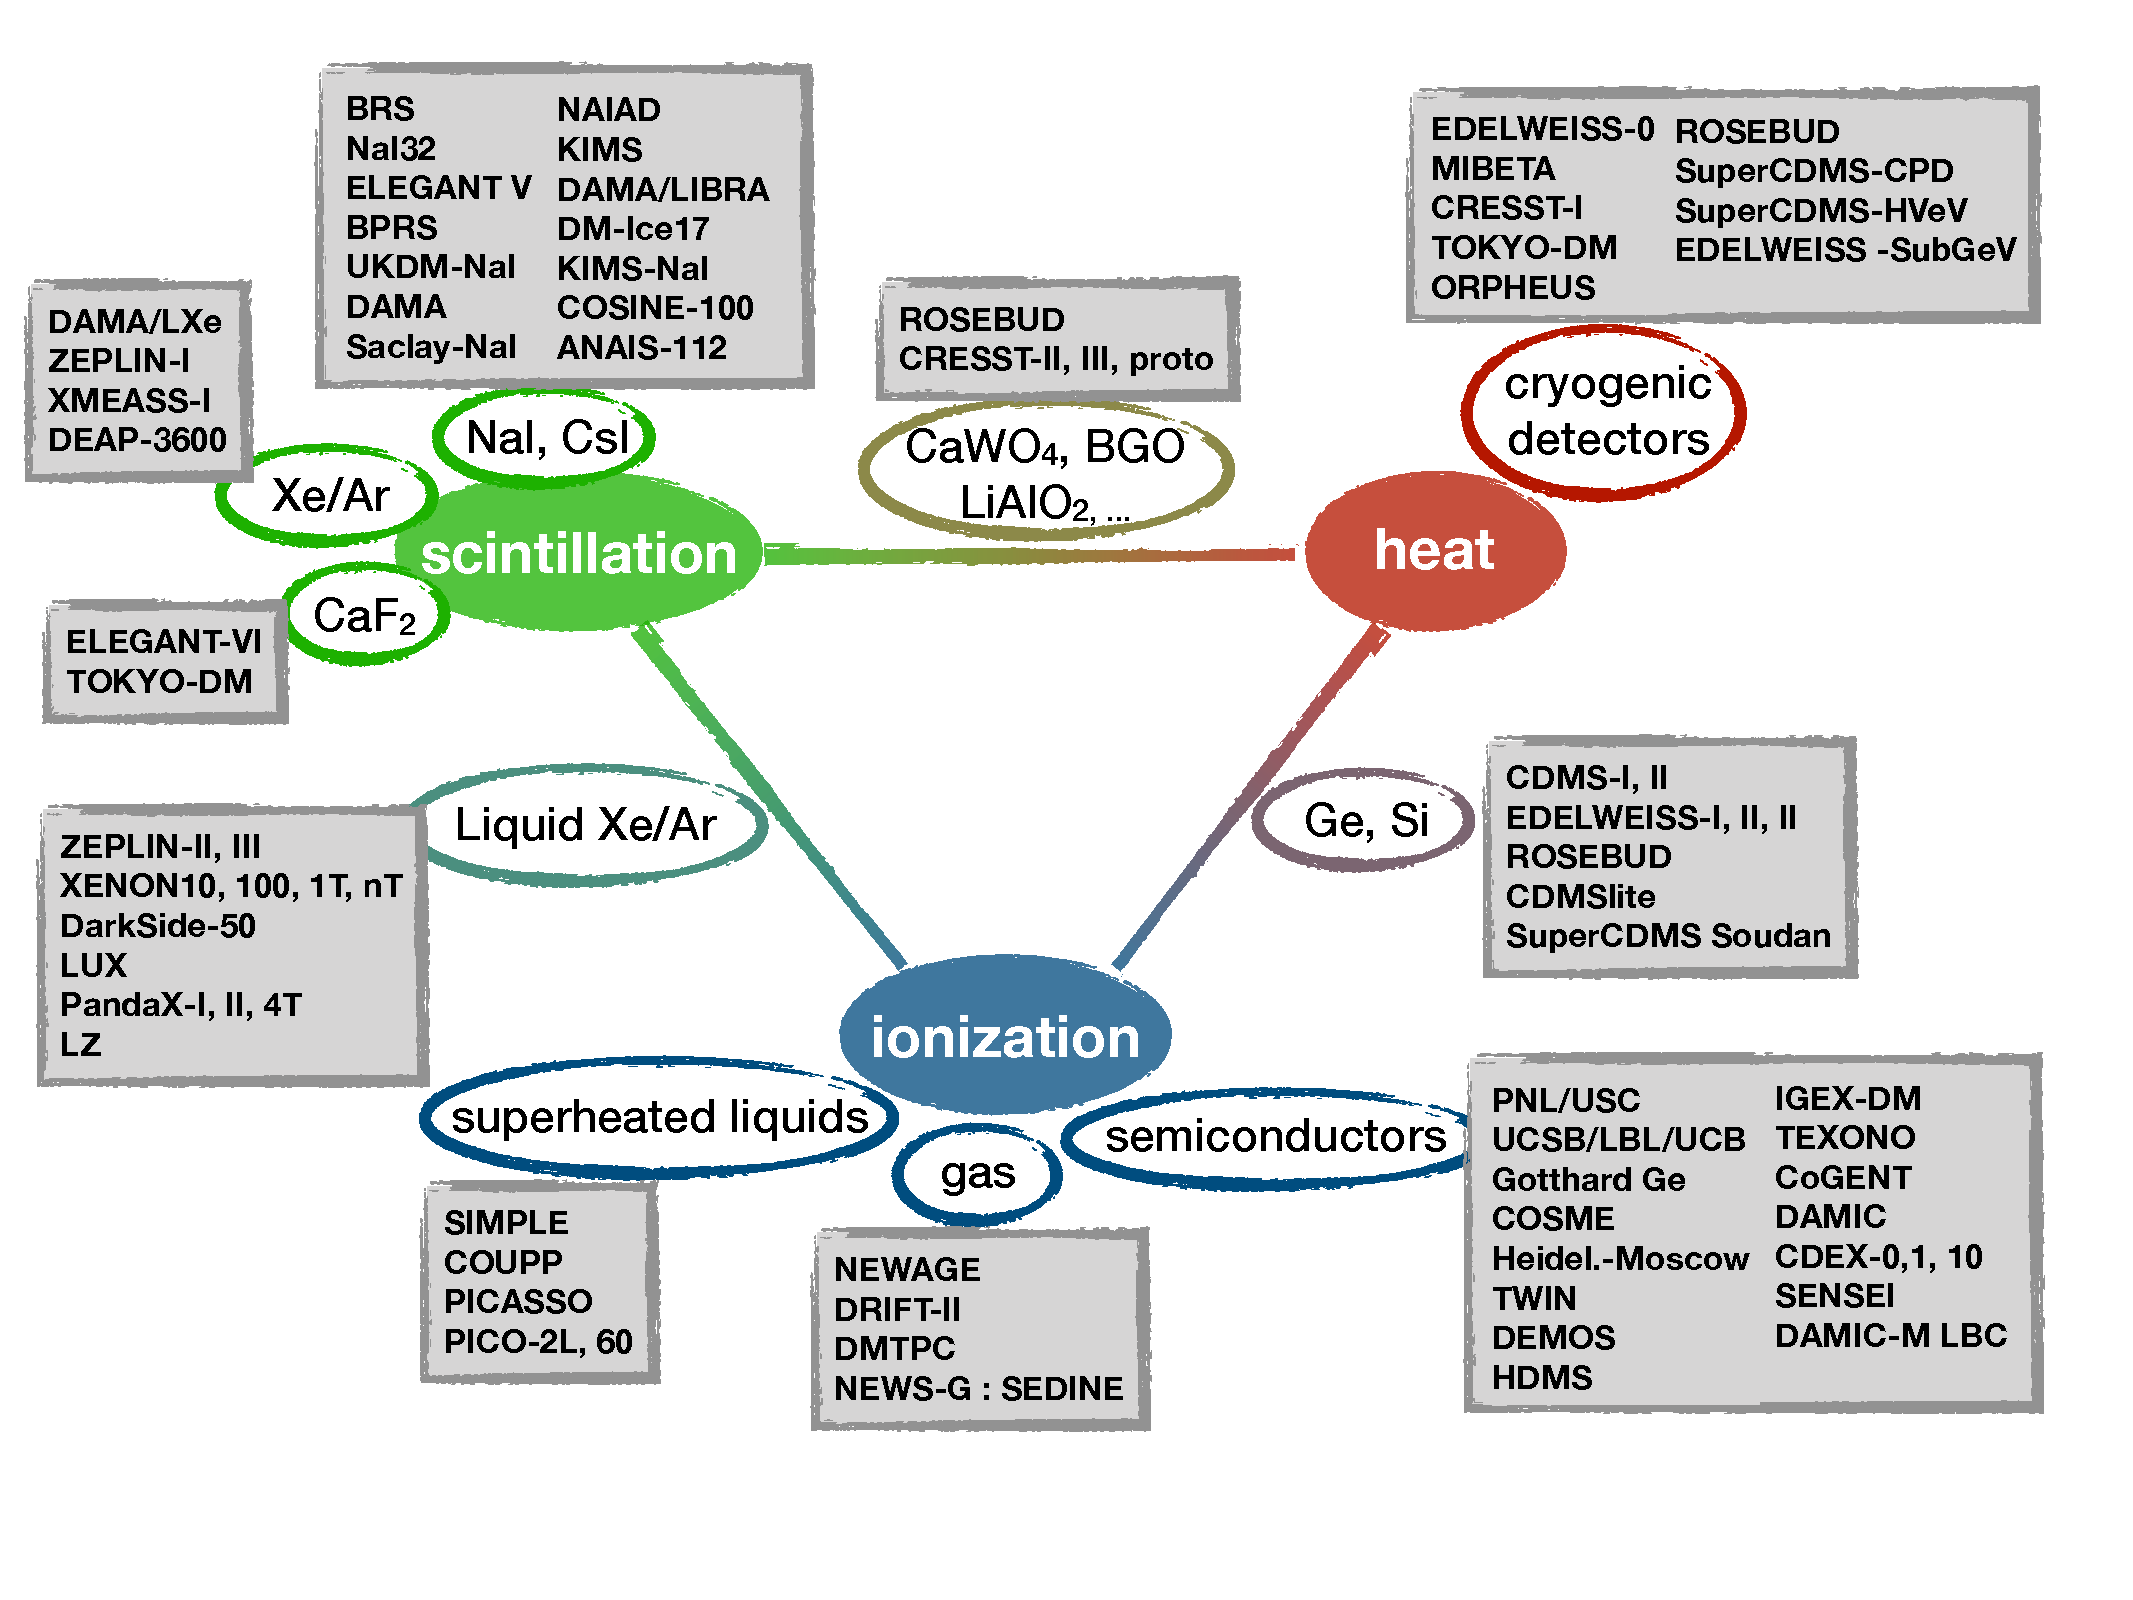
\includegraphics[width=0.9\textwidth]{figs/DM_triangle} 
\end{center}
\caption[Different DM direct detection techniques.]{\em An illustration of different  {\bfseries techniques for DM direct detection}, relying on three different ways of measuring the recoil energy deposited in the scattering on target: scintillation, heat and ionization.} 
\label{fig:DMtriangle}
\end{figure}

\medskip

The energy deposited in DM scattering is observed either as {\em heat, scintillation}, or {\em ionization}. 
That is, the struck nucleus travels through the material and looses energy either by inducing motion of other atoms in the target 
(heat --- in crystals these are the thermal phonons), while a smaller amount of energy loss goes toward exciting or ionizing target atoms. The de-excitation of atoms leads to scintillation light. Either of the three channels can be picked up by appropriate sensors. While historic experiments relied on just one type of signal, many of the more recent experiments read two out of three, and none all three, 
 see fig.~\ref{fig:DMtriangle} and tables \ref{tab:DDexp:hist}, \ref{tab:DDexp}, \ref{tab:DDexp:fut}.
 
 \smallskip
 
  Furthermore,  the response of the detector is different for scattering on electrons and nuclei. The struck electrons lose energy more slowly while traversing the material, and induce almost exclusively a combination of ionization and scintillation.  For detectors sensitive to ionization and/or scintillation but not heat, an electron recoil results in a much higher visible signal than a nuclear recoil event does (in the latter most of the energy goes into heat).  For such detectors it is conventional to present results in terms of 
\beq
\label{eq:quench}
E_{\rm ee}({\rm keV}_{\rm ee})=Q_F \times E_R({\rm keV}_{\rm nr}),
\eeq
where $E_{\rm ee}$, quoted  in keV${}_{\rm ee}$ (keV electron-equivalent), is the would-be energy of an electron recoil that would have resulted in the same detector response as the
nuclear recoil of energy $E_R$ (quoted in keV${}_{\rm nr}$).
The ratio between the two defines the quenching factor, $Q_F$, which in general depends on $E_R$. 
The reason for this bizarre choice of units is that it is straightforward to obtain the response of a detector to electron recoils by using one of several $\gamma$ ray sources of well known energy. This gives the energy calibration of the detector in  keV${}_{\rm ee}$. 
Obtaining the detector response to nuclear recoils is more involved. 
One either needs to perform a dedicated measurement using a mono-energetic neutron source or obtain $Q_F$ from theory. For detectors that are sensitive to the deposited heat, the quenching factor in eq.~\eqref{eq:quench} is irrelevant, and the results can be quoted directly using $E_R$. 

The technologies used in DM direct detection can be grouped in terms of 
cryogenic detectors, scintillating crystals, noble liquid detectors, superheated liquids,  and directional detectors, see also fig.~\ref{fig:DMtriangle}. 
Next, we will discuss in more detail each of these technologies (for other reviews see the Direct Detection part of the reference list in~\cite{otherpastDMreviews}).

\subsection{Cryogenic detectors}\index{Direct detection!cryogenic}
Cryogenic detectors are kept at temperatures well below the room temperature. 
They can accurately measure the energy transferred to the nucleus after the DM scattering event. 
The relative importance of the three signals --- phonons, ionization and scintillation --- depends on the detector material, the detector design, as well as on the read-out. For instance, for a very large detector both ionization and scintillation eventually convert to heat, i.e.,\ phonons. Furthermore, the distribution of the signal among phonons, ionization and scintillation is different for DM (or neutron) scattering and for electron scattering. 
Measuring a signal in two out of three channels is thus an efficient way of reducing the backgrounds.  

\subsubsection*{Ionization detectors} \index{Direct detection!ionization}
The pioneering DM detectors, and some of the more recent cryogenic detectors such as TEXONO  and CoGeNT, were operated as single parameter detectors, utilizing only the ionization channel, see table \ref{tab:DDexp:hist}. 
These were the first detectors to search for DM through direct detection, starting in the late 1980s, as repurposed detectors, originally used in the searches for neutrinoless double $\beta$ decay.  These ionization detectors are semiconductor detectors made out of germanium, operated at the liquid nitrogen temperature of 77$\,$K.  
The energy from nuclear recoil in the  DM scattering event partially goes to excite electrons from the valence band to the conduction band. 
For instance, the quenching factor in Ge is about $Q_F\sim 25$\%. 
This means that an ionization signal  of $1$ keV${}_{\rm ee}$ in the observed energy comes from a nuclear recoil energy of $4$ keV${}_{\rm nr}$.  
The excitation energy required to create a single electron--hole pair is low, ${\mathcal O}(1\eV)$, so that a typical DM scattering event results in many charge carriers, about ${\mathcal O}(300/{\rm keV})$. 
Because of this, the ionization detectors have good energy resolution and low energy thresholds. 
They apply a high voltage $\sim \keV$, to collect all the deposited charge, which, on the other hand, makes  difficult the measurements of the heat deposition in terms of phonons. 


\subsubsection*{Ionization phonon bolometers} 
The CDMS and EDELWEISS collaborations developed Ge and Si detectors that simultaneously measure  the ionization and phonon signals. 
Since the detectors are operated at mK temperatures a discrimination between nuclear and electron recoils is possible even for few keV recoil energies. An important systematic is the incomplete charge collection from the scatterings that occur close to the surface. The collaborations were able to reduce this background with special interleaved electrode readouts. The new SuperCDMS detectors
are expected to reach low thresholds, of $10\,{\rm eV}_{\rm ee}$ for phonons. 


\subsubsection*{Scintillation phonon bolometers} 
The CRESST collaboration developed detectors on CaWO${}_4$ crystals that can measure both the scintillating and phonon signals. The light yield, the ratio of the scintillation and phonon signals, is used to discriminate different scattering types ---  the neutron or DM scattering from the electron or $\gamma$ backgrounds. 
DM can scatter on any of the three nuclei, calcium ($Z=20, A\approx 80$), tungsten ($Z=74, A\approx 180$), or oxygen ($Z=8, A=16$), so that one detector combines light and heavy nuclear targets.  The light yield for DM scattering differs slightly for each of the three cases, which needs to be taken into account in the analysis. The main goal of the CRESST collaboration in recent years was to lower the energy thresholds to below $100\,{\rm eV}_{\rm nr}$ in order to increase sensitivity to sub-GeV DM.



\subsection{Scintillating crystals}
\index{Direct detection!experiment!scintillation}

The scintillating inorganic crystal used in DM detection is most commonly NaI(Tl), and, less commonly, CsI(Tl). Both of these types of detectors are usually operated at room temperature. The DM detection mechanism relies on the fact that part of the nuclear recoil energy from the DM scattering event is converted into scintillation light.  When the recoiled nucleus 
 traverses the scintillating material, it excites the atoms, which then de-excite by emitting light. The NaI and CsI crystals are doped with thalium. This creates defects in the crystal lattice, increasing the light output of the scintillator. It also shifts the emitted light to longer wavelength, at which the crystals are more transparent, while at the same time the light can also be detected with higher efficiency using photosensors. 

The detectors based on NaI(Tl) and CsI(Tl) scintillators have several advantages. The crystals have high mass density, so that it is possible to build targets with large mass. They have high light output, which translates into good energy resolution, and have lower energy thresholds than other scintillators. The detectors are also relatively simple, making it easier to achieve stable operating conditions over periods of several years. The disadvantage is that the energy deposition is measured only in one channel, scintillation, so  it is harder to reject backgrounds. 
This is not possible on  event by event basis, but only statistically, using the fact that the DM signal should exhibit an annual modulation, which for the spin-independent interactions would peak at or around June 2nd. 

Such a signal is claimed with 13$\sigma$ significance in the combined DAMA and DAMA/LIBRA datasets obtained using the ultra low radioactive NaI(Tl) crystals operated at the LGNS laboratory over a period of 14 annual cycles \cite{DAMA,DAMA/LIBRA}. A comparison with the other experiments that do not see a DM signal excludes the DAMA measurement to be due to DM, see section \ref{sec:DAMA}.
In particular, a model-independent check of DAMA signal is possible using the same inorganic scintillator, NaI(Tl). Such detectors are DM-Ice17 operating at  the South Pole since 2011 \cite{1602.05939}, the COSINE experiment at Yangyang, South Korea  and the experiment SABRE in construction, with two detectors, in the south and north hemispheres \cite{SABRE}.
If DM is assumed to scatter on iodine, a model independent check is provided also by CsI(Tl) scintillators,  used in the KIMS experiment at Yangyang, S.\ Korea  \cite{KIMS}.


\subsection{Noble liquid detectors}
\index{Direct detection!experiment!noble liquid}

For a large range of DM masses the most stringent constraints on DM scattering  at present come from the detectors using noble liquids, see fig.s~\ref{fig:sigmaSIbound} and \ref{fig:DDSDbounds}. These type of detectors have several advantages, including a reasonably straightforward scalability to bigger target masses. An important asset of 
detectors based on liquid xenon (LXe) and liquid argon (LAr) is that they can measure the signal from DM scattering in two channels, ionization and scintillation. The scintillation signal originates from excited atoms  that form dimers, ${\rm Xe}_2^*$ and ${\rm Ar}_2^*$. These de-excite to a dissociate ground state, $2 {\rm Xe}$ and $2 {\rm Ar}$, emitting in the process photons with wavelengths of 178 nm and 128 nm, respectively. 
Scintillation efficiency is an important input describing how detectors respond to DM scattering, and is measured in dedicated experimental set-ups. The relative scintillation efficiency, $L_{\rm eff}$, gives the scintillation light yield of nuclear recoils compared to electron recoils of the same energy. It is significantly lower than 1, signifying that electron recoils are much more efficient in producing the scintillation signal. Furthermore, $L_{\rm eff}$ decreases for smaller recoil energies. It equals, for instance, $L_{\rm eff}\approx 0.1$ in  Xe for $E_{\rm nr}\approx$ 10 keV, see, e.g.~\cite{1104.2587,LUX}.  
For very low recoil energies, $E_{\rm nr}\approx$ 1keV, $L_{\rm eff}$ is still rather uncertain, and is an important systematic uncertainty when interpreting the scattering cross section bounds for DM masses below $M\lesssim 10$ GeV. In contrast, the ionization charge yield  of nuclear recoils, in $e^-/{\rm keV}_{\rm nr}$, increases for low-energy recoils. This helps in detecting recoils of GeV or sub-GeV DM. 

\begin{figure}[t]
\begin{center}
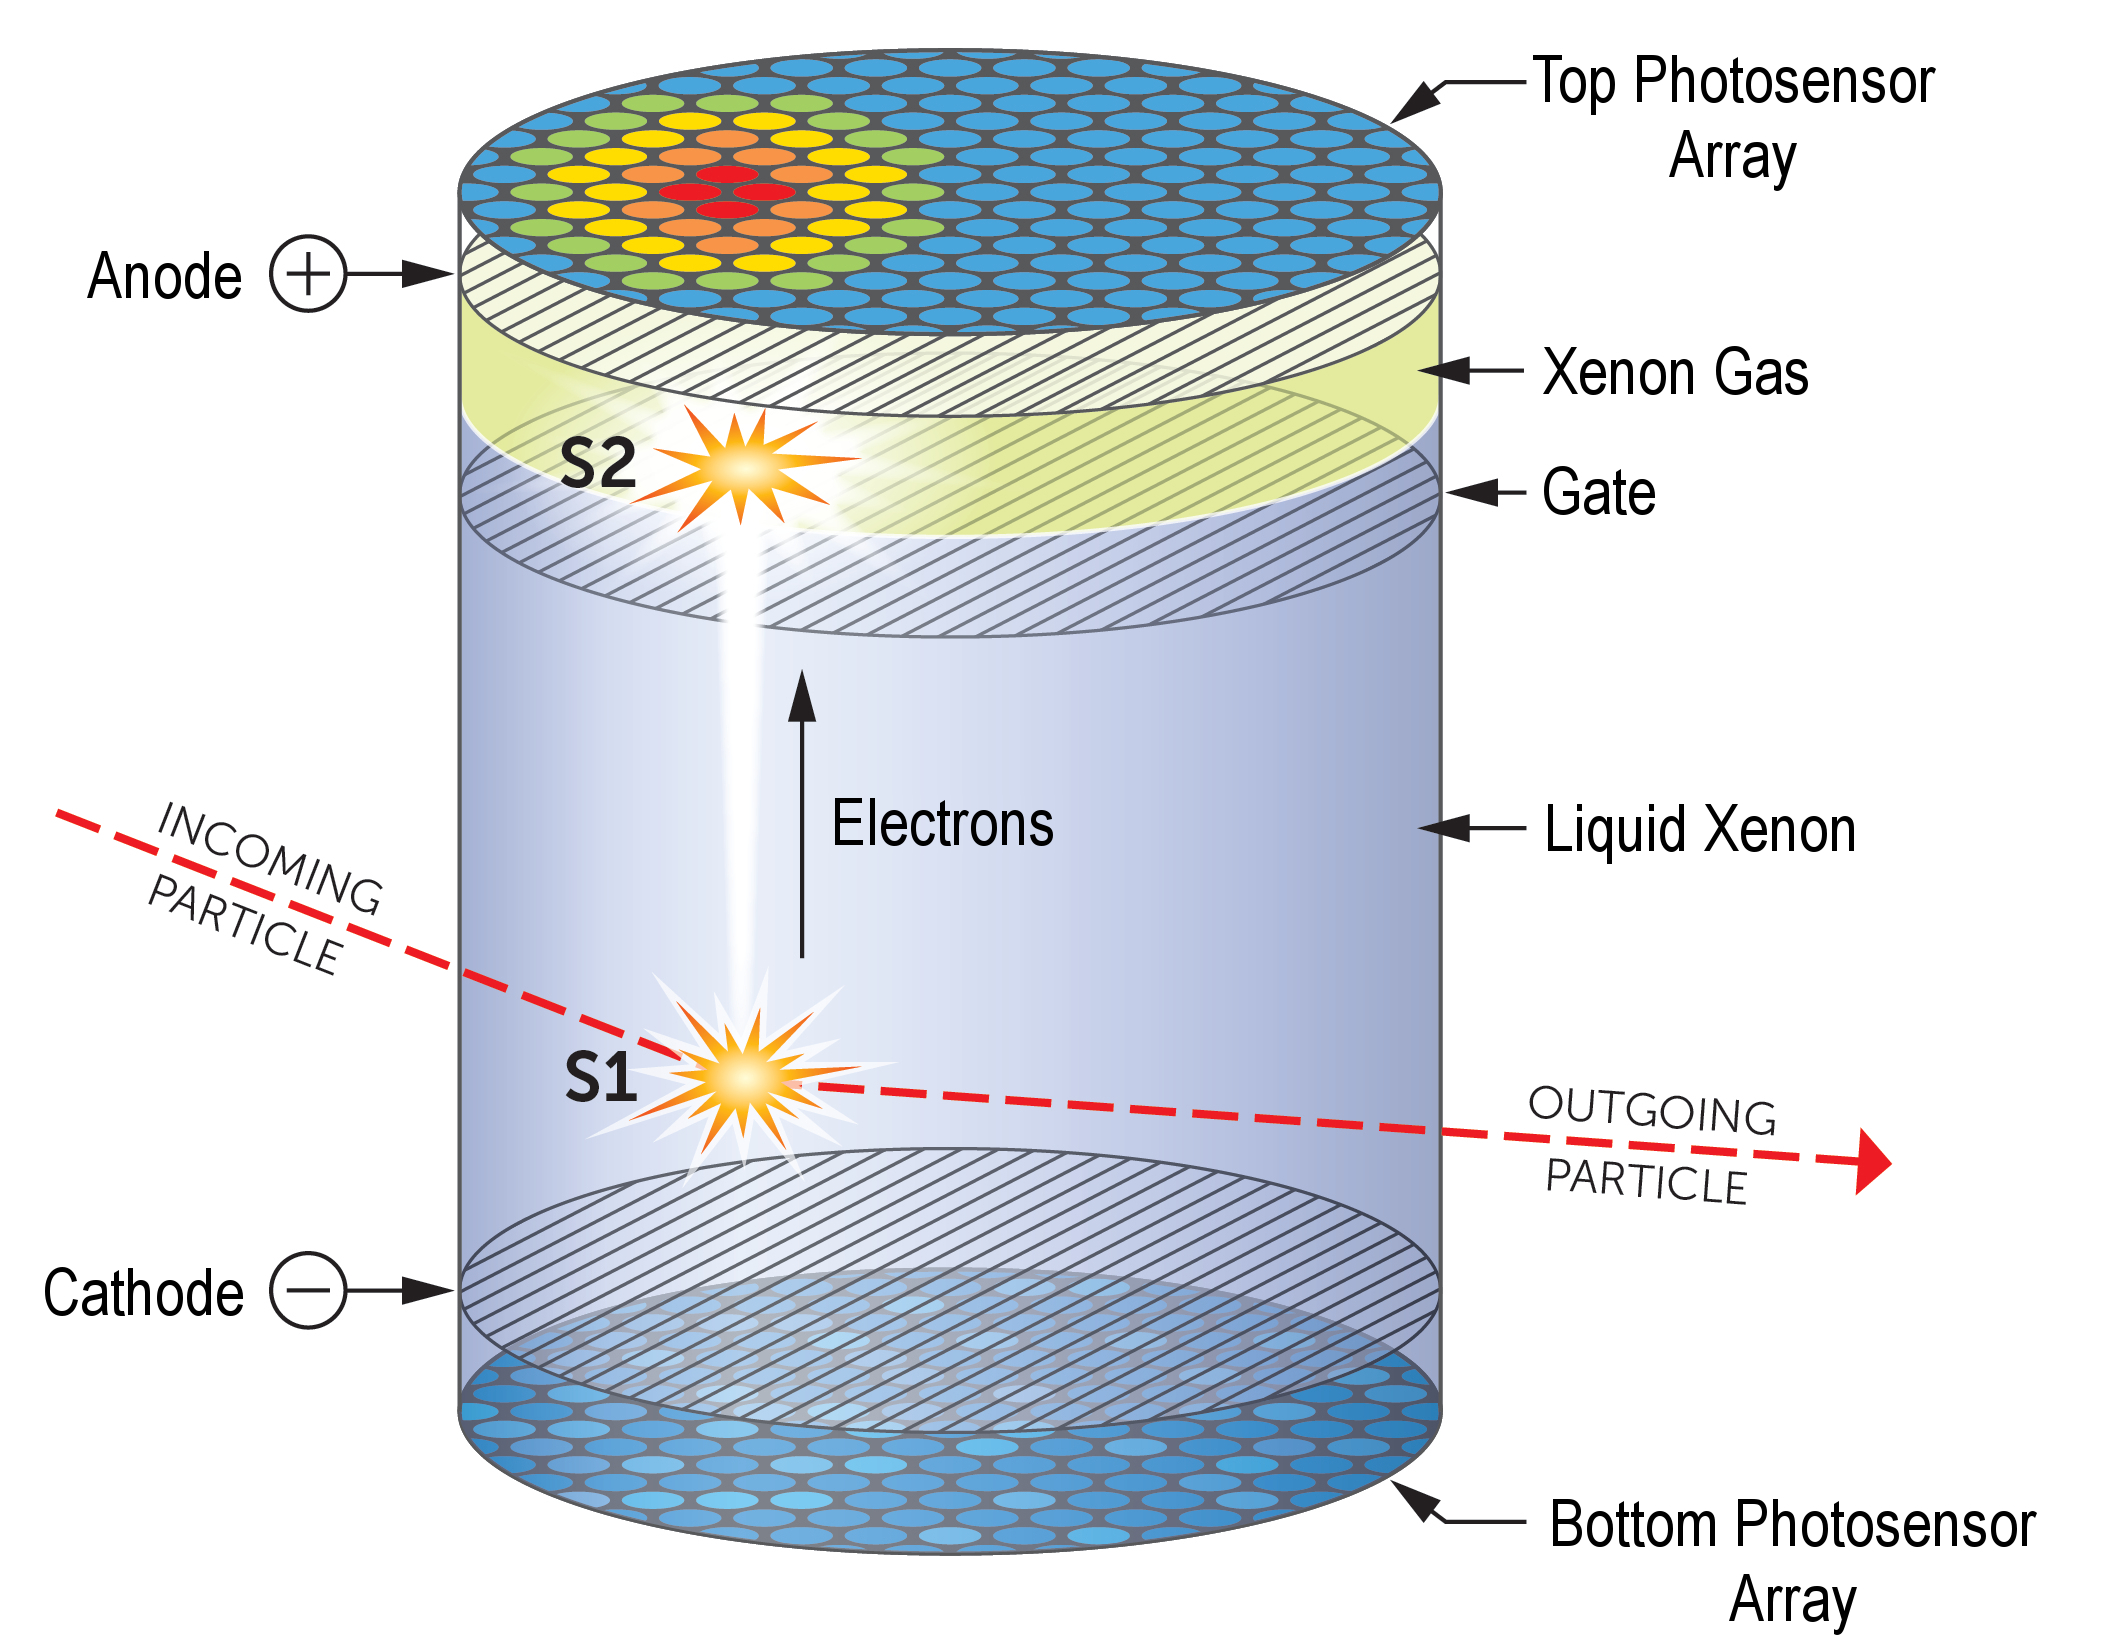
\includegraphics[width=0.53\textwidth]{figs/dual_phase_TPC} 
\end{center}
\caption[Schematics of dual phase TPC detector]{\em The schematics showing the principles of a {\bfseries noble liquid/noble gas dual phase TPC detector}, giving prompt S1 scintillation and delayed S2 ionization signals. Figure from \arxivref{2203.02309}{J.~Aalbers et al.~(2022)} in~\cite{1606.07001}.}
\label{fig:dual:phase:TPC}
\end{figure}

\smallskip

A typical design of the LXe  (or LAr) detectors is a two-phase time projection chamber (TPC). The bulk of the detector is LXe, with gaseous Xe layer on top, see fig.~\ref{fig:dual:phase:TPC}. DM scattering on LXe in the active volume of the TPC creates both scintillation light and the ionization electrons. The scintillation light is collected by the photo-multiplier tubes (PMTs) at the perimeter of the detector, giving the prompt ``$S1$'' signal. 
Under the influence of external electric field, the ionization electrons drift in pure LXe toward the gaseous Xe layer, get accelerated in it by an additional electric field, emitting proportional scintillation photons in the process. This gives the ``$S2$'' signal, delayed by the drift time. 
Since the drift velocity is constant for given electric field, the delay gives the $z$ position of the DM scattering event, while the $x$ and $y$ coordinates are determined by the position of the hits in the PMTs. Furthermore, the $S2/S1$ ratio is an important discriminator of DM signal over backgrounds, since nuclear recoils and electron recoils have very different $S2/S1$ values, $(S2/S1)_{\rm nr}\ll (S2/S1)_{\rm ee}$. 
The 3D positioning of the scattering events allows to cut out the events close to the boundary of the detector, 
utilising the self-shielding property of Xe (in LXe the ambient radiation does not propagate very far). The recent two phase TPC experiments are LUX \cite{LUX}, {\sc PandaX-4T}~\cite{PandaX-4T}, XENON1T \cite{Xenon-1T} and XENONnT \cite{Xenon-nT}\ for Xe, and DarkSide-50 \cite{DarkSide-50}, ArDM \cite{ArDM}  for Ar.
The single phase experiments, XMASS  using LXe \cite{XMASS-I}, and DEAP-3600  using LAr \cite{DEAP-3600}, only measure the scintillation signal $S1$. 
These detectors benefit from a simpler design since there is no need for external electric fields, but the rejection against the backgrounds is harder. Therefore, all the upcoming and planned LXe and LAr experiments are of the dual phase type.

The dual phase design also allows to search for DM scattering or DM absorption on electrons, using the ``$S2$ signal only'' searches, at the cost of larger backgrounds. Similar types of analysis also allow for sub-GeV DM scattering on nucleons through the Migdal effect, see section \ref{sec:Migdal}.


\subsection{Superheated liquids}
\index{Direct detection!experiment!superheated liquid}

The detectors based on superheated liquids are ``yes or no'' types of detectors~\cite{Pullia:2014vra}. The largest such detectors are operated as bubble chambers. A small deposit of energy due to DM scattering on a nucleus triggers a phase transition, creating a bubble of gas, but only if enough energy is deposited locally.
 A commonly used material is C${}_3$F${}_8$ or other liquids that contain fluorine. The most common fluorine isotope, ${}^{19}$F, has an unpaired proton. Thus, there is an enhanced sensitivity to spin-dependent DM/nucleus interactions due to a large corresponding hadronic matrix element.

\smallskip

The readout is in two channels: optical (searching for visible bubbles) and acoustic (measuring the pressure waves from the collapse of the bubbles).  In order for bubbles to be created, the ionization density needs to be above a certain threshold. The DM interactions, neutron interactions or passing $\alpha$ particles ionize above the threshold, while the electromagnetic backgrounds, $\beta$ particles and $\gamma$'s, are below the threshold. Acoustic discrimination can be used to reject the $\alpha$ particle background, since the corresponding signal is louder than the one from DM scattering. The target volume is also monitored visually with digital cameras, detecting the formation of bubbles and their positions. In this way one can reject the surface events, which are more likely to be backgrounds.

Several different versions of detectors based on superheated liquids have been developed. In the past, the experiments with bubble chambers, described above, were the domain of the COUPP collaboration~\cite{1204.3094}.  
A different approach, based on superheated droplets embedded in a gel structure, was developed by SIMPLE \cite{1404.4309} and PICASSO  \cite{1611.01499} collaborations. These types of detectors are more stable and cheaper, but have the downside that only a small part, a few percent, of the detector mass is the target material. The PICASSO and COUPP collaborations merged into PICO collaboration that is operating in SNOLAB a 60 kg bubble chamber of C${}_3$F${}_8$ \cite{1510.07754,1702.07666}. A 40\,l chamber is under construction, while  in the future a 500\,l chamber is planned, see table \ref{tab:DDexp:fut}.  A new concept for the bubble chamber, based on the ``Geyser'' technique, where the vapour above the liquid is kept at a lower temperature, is being developed by the MOSCAB collaboration \cite{1708.00101}. Such detectors have, unlike the conventional bubble chambers, a very short reset time of a few seconds since the bubbles float to the top of the vessel, and then exit the liquid. In contrast, in the conventional bubble chambers one gets rid of the bubbles by increasing the pressure, which is a longer process. 


\subsection{The irreducible neutrino background}
\label{nubck}
\index{Direct detection!neutrino background}
\index{Neutrino!floor/fog/background in DD}

Coherent neutrino/nucleus scattering is an irreducible background to direct DM searches~\cite{nubckg}.
The neutrino/nucleus cross section for neutrinos with energy $E_\nu \circa{<}\GeV$  
is approximately given by
\beq 
\sigma_{\nu A} \approx \frac{\GF^2}{4\pi}N^2 E_\nu^2 F^2(q),
\eeq
where $N$ is the number of neutrons in the nucleus, and $F(q)\approx 1$ is the nuclear form factor for the SI scattering, cf. eq. \eqref{eq:dsigmaAdER}. The neutrino/electron scattering cross section is similarly
\beq 
\sigma_{\nu e} \approx \frac{\GF^2}{4\pi}Z^2 E_\nu^2.
\eeq



The solar neutrinos are the dominant background to DM--nucleus scattering for  DM with a mass below $M\lesssim 10$~GeV,  and for DM scattering on electrons, while the atmospheric and  diffuse supernova background neutrinos are important for heavier DM masses, see fig.s~\ref{fig:sigmaSIbound}, \ref{fig:DDSDbounds}, \ref{fig:DDSIelec:bounds}. In the greyed out regions in the figures the neutrino background is important, and leads to the expected bounds on DM scattering to scale  as 1/(exposure)${}^{1/2}$, instead of the  1/(exposure) scaling in the absence of backgrounds.


A DM signal due to SI scattering on a nucleus can be almost perfectly mimicked by the solar neutrino scattering, so that this background is sometimes referred to as the {\em``neutrino floor''} or the {\em ``neutrino fog''}. The solar neutrinos
give recoil energies, $E_R < 2E_\nu^2/m_A$, where $E_\nu$ is in the MeV regime, resulting in $E_R$
smaller than $\sim (4\div 40)\keV$, with the precise number depending on the mass of the nucleus. The  atmospheric neutrinos, created by cosmic ray collisions with the atmosphere, on the other hand, have a lower flux but reach higher energies, such that they will become a problem for heavy DM masses when the bounds reach $\sigma_{\rm SI}/M \circa{<}10^{-48}\cm^2/\TeV$.
Amusingly, the background due to such neutrinos would be smaller
for a detector on the moon, which has almost no atmosphere, while cosmic ray collisions with the lunar surface and crust lead to a less energetic neutrino flux~\cite{2305.04943}.


An important discriminator against the neutrino background could be measurements done with different nuclei. While coherent neutrino scattering is dominated by couplings to neutrons, DM could couple to neutrons and protons with comparable strengths, or even more preferentially to protons, giving differing signals for scatterings on light versus 
heavy nuclei. This strategy is especially powerful, if DM/nucleon interactions are dominated by the spin-dependent scattering, the rate for which is highly dependent on the type of target used in the experiment. 

Another possibility is to develop directional detectors, which we discuss next. In this case one could cut on events originating from the Sun's direction, thus reducing the solar neutrino background. 



\subsection{Directional detectors}
\index{Direct detection!directional}
\label{sec:dir:detection}
The Earth is moving through the DM halo toward  the Cygnus constellation (with Galactic coordinates $\ell \approx 90^\circ$ and $b\approx 0^\circ$), see section~\ref{sec:DM:velocity:Earth}. In the Earth's rest frame there is therefore an apparent DM wind blowing  
from the direction of the Cygnus constellation. Since the DM/nucleus scattering peaks in the forward direction, the nuclear recoils also preferentially originate from the direction of the Cygnus constellation, but with a wider angular spread. 
The directionality of the DM signal can be a discriminator against the otherwise irreducible backgrounds that will be reached in the future, 
such as the events induced by the solar and atmospheric neutrinos (the so called neutrino fog, see section~\ref{nubck}). 
A significant effort is therefore devoted toward developing directional detectors, which may be needed to go below the neutrino fog \cite{1110.6079}. The detectors can have 1D capabilities, i.e.,~only distinguishing the forward scattering from the backward scattering, or the more powerful 2D or the full 3D reconstruction of the nuclear recoil track. In addition, if the information on the progression of the track is available (such as timing or the shape of the tracks), this allows for the head-tail discrimination, i.e., which direction did the track originate from. The signal in directional detectors carries enough information 
that one could simultaneously determine the DM mass, the scattering cross section as well as the DM velocity profile from a single 3D directional detector.

Several types of detectors that have potential directional sensitivity are being developed. Broadly speaking there are two approaches:

\subsubsection*{Direct imaging of the recoil track} 
Gas time projection chambers (TPCs) are the most mature technology. 
The gas needs to be  at low pressure so that the  keV-scale nuclear recoils result in $\sim \text{mm}$ ionization tracks, 
which can then be imaged with fine enough readout approaches. Because of the required low pressure the challenge for the gas TPC is always the small total target mass. The benefit is, beyond reducing backgrounds due to directionality of the signal, that many different types of gases or mixtures of gases can be used: Ne, CH${}_4$, CF${}_4$, CHF${}_3$, C${}_4$H${}_{10}$,..., and thus can be sensitive to different DM interactions. The start of the research dates all the way to early 1990s \cite{Buckland:1994gc}, and is now a global effort, with DRIFT at Boulby mine, UK  \cite{DRIFT-II}, MIMAC in Modane, France\cite{MIMAC}, NEWAGE in Kamioka, Japan \cite{NEWAGE}, DMTPC at MIT, USA \cite{DMTPC}, D${}^3$ at U.\ Hawaii and LBNL, USA \cite{D3}, and CYGNO at Gran Sasso, Italy \cite{CYGNO}. Recently, these groups formed a CYGNUS proto-collaboration, which is exploring a possibility of a ton-scale `recoil observatory' \cite{CYGNUS}. This would reach the neutrino fog for GeV DM masses and potentially push below it. Other, less well developed ideas for DM detectors with directional capabilities are based on emulsions \cite{NEWSdm}, crystal defects \cite{CrystalDefectsDM}, 2D materials \cite{Hochberg:2016ntt,PTOLEMY} and using DNA strands \cite{Drukier:2012hj}. The distribution of tracks could potentially also  be used to search for a weak scale DM signal in the ``paleo-detectors'', i.e., the deep underground mineral rock samples with Gyr exposures (scanning of mica slabs was already used to set limits on ultraheavy DM, which would deposit the easier  to distinguish long tracks) \cite{Paleodetectors}. In general, in emulsions and solids there is a significant spread in the movement of the recoiled nucleus in the transverse direction, while in the low pressure gas environment of TPCs the directionality of the recoiled nucleus is much better preserved. Consequently, most of the research and development has focused on various versions of  the gas TPCs.  \index{Paleo-detectors}

\subsubsection*{Indirect directional detection} 
Even if the tracks from the individual DM scattering are not reconstructed, one can still gain some directional information on a statistical basis, if the response of the detector is anisotropic \cite{AnisotropicScint,2212.04505,Columnar:Recombination}. Anisotropic scintillators, such as ZnWO${}_4$, have a light yield that depends on the recoil direction relative to the crystal axes \cite{AnisotropicScint}. This can then be correlated with the expected direction of the DM wind, taking into account both the annual and daily modulation, in order to increase the significance of the DM scattering signal. Interestingly, there is also some asymmetry in the ionization and scintillation responses of liquid argon (and potentially xenon) detectors due to the applied electric field, though the asymmetry is probably too small to significantly aid DM searches~\cite{Columnar:Recombination}. 



\subsection{Searches for scattering on electrons}
\label{sec:electron:DMscatter}

\begin{table}[t]
\begin{center}
\setlength\tabcolsep{1pt} \renewcommand{\arraystretch}{0.95}
\resizebox{\columnwidth}{!}{
\begin{tabular}{ccccccc}
\hline
\hline
 {\bf Experiment} & {\bf Location} & {\bf Operation} & {\bf Technology} &{\bf Target Mass} & {\bf Home} & {\bf Ref.}   \\
\hline

\multirow{2}{*}{\sc CDMS II} & \multirow{2}{*}{Soudan, MN} & \multirow{2}{*}{2006 $\to$ 2007 } &  \multirow{2}{*}{ath. phon.+ioniz. (50\,mK)$\Big\{$} & $4.6\,$kg  Ge &  \multirow{2}{*}{\href{https://www.slac.stanford.edu/exp/cdms/}{web}} & \multirow{2}{*}{\cite{CDMS-II}} 
\\
 &  &  &  & $1.2\,$kg Si &  & 
\\

{\sc XENON10} & Gran Sasso, Italy & 2006 $\to$ 2007 & scint.+ioniz. ($179\,$K)  & 5.4\,kg Xe& \href{http://xenon.astro.columbia.edu/XENON10_Experiment/}{web} & \cite{XENON10}
\\

{\sc EDELWEISS II} & Modane, France & 2009 $\to$ 2010 & ther. phon.+ioniz. (18\,mK) & 4\,kg Ge & \href{http://edelweiss.in2p3.fr}{web} & \cite{EDELWEISS-II}
\\
{\sc KIMS} & Yangyang, S. Korea & 2009 $\to$ 2012 &  scint. ($\sim300\,$K) & $103.4$\,kg CsI(Tl) & \href{https://web.archive.org/web/20200218154113/http://q2c.snu.ac.kr/KIMS/KIMS_index.htm}{web} & \cite{KIMS}
\\

{\sc EXO-200} & Carlsbad, NM & 2011 $\to$ 2018 &  scint.+ioniz. ($\sim167\,$K) & $82$\,kg Xe & \href{https://www-project.slac.stanford.edu/exo/}{web} & \cite{EXO-200}
\\

{\sc CDMSlite} & Soudan, MN & 2012 $\to$ 2014 & ath. phon.+ioniz. $(\sim50\,$mK)& $0.6\,$kg Ge & \href{https://supercdms.slac.stanford.edu}{web} & \cite{CDMSlite} \\

{\sc XMASS-I} & Kamioka, Japan & 2013 $\to$ 2017 &  scint. $(173\,$K) & 832\,kg Xe & \href{http://www-sk.icrr.u-tokyo.ac.jp/xmass/index-e.html}{web} & \cite{XMASS-I}
 \\
 
  {\sc DarkSide-50} & Gran Sasso, Italy & 2013 $\to$ 2018 &  scint.+ioniz. $(\sim80\,$K)  &  46\,kg Ar & \href{http://darkside.lngs.infn.it}{web} & \cite{DarkSide-50} \\
 
 {\sc LUX} & Sanford, SD & 2013 &  scint.+ioniz. $(\sim180\,$K)  & $118\,$kg Xe & \href{http://luxdarkmatter.org}{web} & \cite{LUX}
 \\
 {\sc EDELWEISS-III} & Modane, France & 2014 $\to$ 2015 &  ther. phon.+ioniz. $(18\,$mK) & $\sim16.5\,$kg Ge & \href{http://edelweiss.in2p3.fr}{web} & \cite{EDELWEISS-III}
\\

 {\sc CDEX-1} & Jinping, China & 2014 $\to$ 2017 &  ioniz. $(\sim90\,$K) & 0.9\,kg Ge &  \href{http://cjpl.tsinghua.edu.cn/publish/jinping/903/index.html}{web} & \cite{CDEX-1}
\\
{\sc PandaX-II} & JinPing, China & 2015 $\to$ 2018 &  ioniz.+scint. $(\sim165\,$K) & $\sim117$\,kg Xe &  \href{https://pandax.sjtu.edu.cn}{web} & \cite{PandaX-II} 
\\


{\sc DAMIC} & SNOLAB, Canada & 2016 $\to$ 2017  &  ioniz. $(\sim105-140\,$K)& $6\to40\,$g Si &  \href{http://damic.uchicago.edu}{web} & \cite{DAMIC} \\

\multirow{2}{*}{{\sc SENSEI}~~$\Big\{$} & Fermilab, IL & 2017 $\to$ 2020 &  ioniz. $(130\,$K) & $95\,$mg $\to 1.9$\,g Si &  \multirow{2}{*}{\href{https://sensei-skipper.github.io}{web}} & \multirow{2}{*}{\cite{SENSEI}}
\\
& SNOLAB, Canada & 2022 $\to$  &  ioniz. $(130\,$K) & $\sim 100$\,g Si &   & 
\\

\multirow{2}{*}{{\sc SuperCDMS-HVeV} $\Big\{$} & Stanford, CA & 2017 & ath. phon. $(36\,$mK)  & $1\,$g Si & \multirow{2}{*}{\href{https://supercdms.slac.stanford.edu}{web}} & \multirow{2}{*}{\cite{SuperCDMS-HVeV}} \\
 & Northwestern, IL & 2019 & ath. phon. $(36\,$mK)  & $1\,$g Si & &  \\
 
{\sc CDEX-10} & Jinping, China & 2017 $\to$ 2018 &  ioniz. $(\sim 90\,$K) & $0.9$\,kg Ge&  \href{http://cdex.ep.tsinghua.edu.cn}{web} & \cite{CDEX-10} \\

{\sc XENON1T} & Gran Sasso, Italy & 2017 $\to$ 2018 & ioniz.+scint. (177\,K) & $1042$\,kg Xe & \href{http://www.xenon1t.org}{web} & \cite{Xenon-1T} 
\\

{\sc Blanco et al.} & Chicago, USA  & 2018 &  scint. (274\,K) & 1.3\,kg $\text{C}_8\text{H}_{10}$ & \href{https://doi.org/10.1103/PhysRevD.101.056001}{paper} & \cite{DM:electron:organic:scint}
\\

{\sc Hochberg et al.} & MIT, USA  & 2018 & supercond. nanowire (300\,mK) & 4.3\,ng WSi& \href{https://journals.aps.org/prl/pdf/10.1103/PhysRevLett.123.151802}{paper} & \cite{DM:electron:superconductors:nanowiresHochberg}
\\

{\sc EDELWEISS-SubGeV} & Modane, France & 2019 & ther. phon. (20\,mK) & 33.4\,g Ge& \href{http://edelweiss.in2p3.fr}{web} & \cite{EDELWEISS-SubGeV}
\\

{\sc LAMPOST} &  MIT, USA & 2021 & supercond. nanowire (300\,mK) & ${\mathcal O}$(4\,ng) WSi& \href{http://edelweiss.in2p3.fr}{paper} & \cite{LAMPOST}
\\

{\sc PandaX-4T} & Jinping, China & 2021 $\to$ &  ioniz.+scint. $(\sim 170\,$K) & 2.7\,t Xe & \href{https://pandax.sjtu.edu.cn}{web} & \cite{PandaX-4T}\\
{\sc XENONnT} & Gran Sasso, Italy & 2021 $\to$  &  ioniz.+scint. (177\,K) & 4.4\,t Xe & \href{http://www.xenon1t.org}{web} & \cite{Xenon-nT}\\

 {\sc DAMIC-M LBC} & Modane, France & 2022 $\to$ &  ioniz. $(\sim130\,$K) & $8$\,g Si &  \href{http://damic.uchicago.edu}{web} & \cite{DAMIC-M-LBC} \\
 
  {\sc JWST NIRSpec} & Lagrange point L2 & 2022 $\to$ &  ioniz. $(43\,$K) & $21$\,kg Hg${}_{0.7}$Cd${}_{0.3}$Te &  \href{https://jwst-docs.stsci.edu/jwst-near-infrared-spectrograph}{web} & \cite{JWST NIRSpec} \\
  
   {\sc DAMIC-M} & Modane, France & 2024 $\to$ &  ioniz. $(\sim120\,$K) & $26.4$\,g Si &  \href{http://damic.uchicago.edu}{web} & \cite{DAMIC-M} \\

\hline\hline
\end{tabular}}
\end{center}
\caption[electron scattering]{\em The past and present {\bfseries direct detection experiments} bounding {\bfseries scattering and/or absorption on electrons}. Experiments are ordered by the year of the first relevant physics run (3rd column), with the 2nd column showing the location, the 4th column the technology used and the 5th column the fiducial target mass.
 The last two columns give references for each experiment.   The abbreviations used are the same as in table~\ref{tab:DDexp:hist}. Planned experiments are listed in table~\ref{tab:DDexp:fut}.
\label{tab:Directional:exp}}
\end{table}

In any material one can have scattering of DM on either nuclei or on electrons, with the relative rates depending on the couplings of DM to electrons or to quarks and gluons. Both types of scattering deposit energy in the detector so in principle one can  search for both using a single detector. 
However, the two types of scattering lead to different signals in detectors, 
so the question is whether experimentally the resulting signal can be picked up, and not be overwhelmed by the backgrounds. The experiments that have searched for DM scattering on electrons fall into two categories. 



In the first group are the experiments that were primarily built to search for DM scattering on nuclei, and would typically treat electron recoils as backgrounds. Even so, lately many were able to place limits on DM/electron scattering by modifying their analyses. The prime examples are dual phase xenon detectors, in which in the nominal analysis the electron recoil events are treated as backgrounds and discarded, while in the $S2$-only analysis these events can be used to search for an excess due to DM scattering on electrons. 


The second group consists of the experiments specifically built to search for DM/electron scattering. 
The prime examples are the SENSEI \cite{SENSEI} and DAMIC \cite{DAMIC} experiments, which use versions of silicon CCDs 
(i.e.,\ improved versions of the CCD sensors that are in everyday digital cameras) as ionization detectors. The energy transfer from DM to the detector is via electron recoil, creating a hole-electron pair, where the hole is captured in a potential well that can be read out repeatedly. This technique leads to very low energy thresholds all the way down to the Si band gap of 1.2\,eV, since one can measure just a single hole--electron creation. This translates to a sensitivity to DM masses down to $\sim$MeV for DM/electron scattering, and to $\sim$eV for DM absorption. 
DAMIC and SENSEI are not directly sensitive to nuclear recoils in DM/nucleon scattering. However, the hole-electron creation can also be interpreted in terms of a Migdal effect in the DM/nucleon scattering, see section~\ref{sec:Migdal}. 
The energy threshold can potentially be lowered by using superconducting nanowires as the target material, which then acts as a sensitive bolometer, changing from superconducting to normal conductor even if very small energies are deposited (the superconducting gap is only $\sim {\rm meV}$). 
The first bounds on DM/electron scattering~\cite{DM:electron:superconductors:nanowiresHochberg} and dark photon absorption \cite{LAMPOST} using superconducting wires were placed already using prototype detectors, presently with comparable reach than the other experiments. 

The experiments that placed limits on DM/electron scattering and/or DM absorption on electrons are listed in table \ref{tab:Directional:exp}.




\subsection{Searches for neutrinos from the Sun and the Earth}\label{sec:DMnustatus}

The capture of DM particles in the center of celestial bodies such as the Sun and the Earth can lead to a signal in terms of high energy neutrinos. As discussed in more detail in section \ref{sec:DMnu}, the flux of neutrinos from the Sun due to DM annihilations is controlled by the DM capture rate, since this is the bottle neck. 
The bounds on neutrino flux from the Sun at energies above tens of MeV (which is high enough that the SM solar neutrino flux is negligible) 
would then impose constraints on DM capture rate, and by extension on the DM/proton scattering cross section, the same quantity that is probed by the conventional direct detection searches discussed above. The neutrino telescopes have higher thresholds,  and therefore place bounds only for GeV DM masses and above.

\medskip

Several neutrino telescopes derived such bounds.
For annihilations in the center of the Sun (for SI and SD scattering): {\sc Antares}~\cite{1603.02228}, {\sc Icecube}~\cite{1612.05949,ColomiBernadich:2019upo,2111.09970}, {\sc KM3NeT}~\cite{KM3NeT:2024xca},
{\sc Baksan}~\cite{1301.1138},
and {\sc SuperKamiokande}~\cite{1503.04858}.
For capture and annihilations in the Earth (SI): {\sc Antares}~\cite{1612.06792},
{\sc Icecube}~\cite{1609.01492},
{\sc SuperKamiokande}~\cite{hep-ex/0404025}.
A selection of these constraints is reported in the plots on direct detection bounds (SI, figure \ref{fig:sigmaSIbound}, and SD, figure \ref{fig:DDSDbounds}). 
The bottom line is that, at the current stage, the constraints from the Sun on the SI cross section are about two orders of magnitude weaker than direct detection constraints. Constraints on the SD cross section are instead stronger than the direct detection constraints by about one order of magnitude (for the leptonic and gauge boson channels).
Future   {\sc HyperKamiokande} data are expected to improve constraints from the Sun by a factor of 2-3~\cite{Bell:2021esh}.
On the other hand, given the current bounds from direct detection, the flux from the center of the Earth is predicted to be too weak to give a relevant signal. 

\begin{table}[!t]
\begin{center}
\setlength\tabcolsep{1pt} \renewcommand{\arraystretch}{0.95}
\resizebox{\columnwidth}{!}{
\begin{tabular}{ccccccc}
\hline
\hline
  {\bf Experiment} & {\bf Location} & {\bf Data Taking} & {\bf Readout} &{\bf Target} & {\bf Home} & {\bf Ref.}   \\

\hline

{\sc DarkSide-20k} & Gran Sasso, Italy & 2026 &  scint.+ioniz. $(\sim85\,$K)  &  20\,t\,Ar & \href{http://darkside.lngs.infn.it}{web} & \cite{1707.08145} \\

{\sc DarkSide-LowMass} & Gran Sasso, Italy &  &  scint.+ioniz. $(\sim85\,$K)  &  $\sim$1\,t\,Ar & \href{http://darkside.lngs.infn.it}{web} & \cite{1707.08145} \\

{\sc SBC} &  SNOLAB, Canada & 2028 & scint. bubble chamb. $(\sim100\,$K) & 10\,kg Ar & \href{https://indico.cern.ch/event/922783/contributions/4892804/attachments/2481892/4260774/Broerman_IDM2022.pdf}{talk} & \cite{SBC} \\

{{\sc ARGO}} & {SNOLAB, Canada} & {2029} &  { scint.+ioniz.}   { $(\sim85\,$K)}  & { 300\,t\,Ar} & \href{http://darkside.lngs.infn.it}{web} & \href{https://indico.cern.ch/event/765096/contributions/3295671/attachments/1785196/2906164/DarkSide-Argo_ESPP_Dec_17_2017.pdf}{web} \\

{ {\sc DarkSide-LM}} &   &   &  { scint.+ioniz. $(\sim85\,$K)} &  {1.5\,t Ar} &  \href{http://darkside.lngs.infn.it}{web} & \cite{DarkSide-LM} \\

{\sc LZ-HydroX} & Sanford, SD & 202x  &  ioniz.+scint. (174\,K) & 5.5\,t Xe + 2\,kg H${}_2$ & \href{https://lz.lbl.gov}{web} &  \href{https://www.snowmass21.org/docs/files/summaries/CF/SNOWMASS21-CF1_CF0_Hugh_Lippincott-106.pdf}{LOI} \\

{\sc XLZD} & undetermined & 203x &  scint.+ioniz. ($\sim 170\,$K) & 60/80\,t Xe & \href{https://xlzd.org}{web} & \cite{1606.07001} \\

{\sc PandaX-20T} & Jinping, China & 2027 &  scint.+ioniz. $(\sim170\,$K) & $\sim 20\,$t Xe & \href{https://pandax.sjtu.edu.cn}{web} & \href{https://indico.global/event/652/contributions/16967/attachments/57462/110370/20250325_PandaX_UCLADM.pdf}{talk} \\

{\sc PandaX-xT} & Jinping, China & 203x &  scint.+ioniz. $(\sim170\,$K) & $\sim 40\,$t Xe & \href{https://pandax.sjtu.edu.cn}{web} & \cite{Liu:2017drf} \\

{\sc QUEST-DMC} &  &  &  quasipart. $(\sim100\,\mu$K) & $1\,$cm${}^3$ ${}^3$He & \arxivref{2310.11304}{paper} & \cite{QUEST-DMC} \\

{\sc DELight} & Vue-des-Alpes, Switz. & 202x &  phon.+roton $(\sim20\,$mK) & $10\,$l ${}^4$He & \href{https://delight.kit.edu}{web} & \cite{DELight} \\

{\sc HeRALD} &  & 202x &  phon.+roton $(\sim50\,$mK) & $\sim1\,$kg ${}^4$He & \href{https://tesseract.lbl.gov/herald/}{web} & \cite{HeRALD} \\

\multirow{2}{*}{{\sc SuperCDMS SNOLAB}} & \multirow{2}{*}{SNOLAB, Canada} & \multirow{2}{*}{~~~~~~2023$\to$~~$\Big\{$} & ath. phon.[+ioniz.]  (15\,mK) & $ 11[+14]$\,kg Ge & \multirow{2}{*}{\href{https://supercdms.slac.stanford.edu}{web}} & \multirow{2}{*}{\cite{SuperCDMS-SNOLAB}} \\

 &  &  & ath. phon.[+ioniz.] (15\,mK) & $ 2.4[+1.2]$\,kg Si &  &  \\
 
  {\sc RES-NOVA} & Gran Sasso, Italy &  &  ther. phon.+ioniz.  & $\sim170\,\text{kg}\to 1.8\,\text{t}$ PbWO${}_4$ & \href{https://arxiv.org/abs/2501.12409}{paper} & \cite{RES-NOVA}
\\
 
 {\sc OSCURA} & SNOLAB, Canada & 2029 &  ioniz. $(\sim130\,$K) & $10$\,kg Si &  \href{http://damic.uchicago.edu}{web} & \cite{OSCURA} \\
 
  {\sc CDEX-50} & Jinping, China & 202x &  ioniz. $(\sim90\,$K) & $\sim 300\,$kg Ge &  \href{http://cdex.ep.tsinghua.edu.cn}{web} & \href{https://indico.ific.uv.es/event/6178/contributions/15871/attachments/9322/12147/Recent_status_and_prospects_of_CDEXCJPL-Litao_Yang-TAUP2021.pdf}{talk} \\

{\sc EDELWEISS-CRYOSEL} & Modane, France & 202x & ath. phon. ($\sim 10\,$mK) & $\sim30$\,g Ge & \href{http://edelweiss.in2p3.fr}{web} & \cite{EDELWEISS-CRYOSEL}
\\
 
 { {\sc CDEX-300}} & {Jinping, China} & {2027} &  {ioniz. $(\sim90\,$K)} & {$\sim 300\,$kg Ge} &  \href{http://cdex.ep.tsinghua.edu.cn}{web}  & \href{http://cdex.ep.tsinghua.edu.cn/upload_files/atta/1657037877563_E8.pdf}{LOI} \\
 
 { {\sc CDEX-1T}} & { Jinping, China } &  {2033}  &  { ioniz. $(\sim90\,$K)} & {$\sim 1$\,t Ge} &  \href{http://cdex.ep.tsinghua.edu.cn}{web} & \href{http://cdex.ep.tsinghua.edu.cn/upload_files/atta/1657037877563_E8.pdf}{LOI}  \\
 
 { {\sc CDEX-10T}} & { Jinping, China } & {2040} &  { ioniz. $(\sim90\,$K)} & {$\sim 10$\,t Ge} &  \href{http://cdex.ep.tsinghua.edu.cn}{web} & \href{http://cdex.ep.tsinghua.edu.cn/upload_files/atta/1657037877563_E8.pdf}{LOI}  \\

{\sc COSINE-200} & Yemilab, South Korea & 2024$\to$ &   scint. ($\sim300$\,K) & $\sim$ 200\,kg NaI(Tl) &  \href{http://cosine.yale.edu/home}{web} & \href{https://indico.sanfordlab.org/event/28/contributions/295/attachments/245/546/CoSSURF_COSINE.pdf}{talk} \\


{\sc COSINE-100U} & Yemilab, South Korea & 2025 &   scint. ($\sim300$\,K) &  99.1\,kg NaI(Tl) &  \href{http://cosine.yale.edu/home}{web} & \cite{COSINE-100U} \\

{\sc COSINUS} & Gran Sasso, Italy & 2025 &  scint. $(\sim10\,$mK)  &  $0.24\to\sim1$\,kg NaI(Tl) & \href{https://cosinus.sites.lngs.infn.it}{web} & \cite{COSINUS} \\

\multirow{2}{*}{{\sc SABRE}~~~~~$\Big\{$} & Gran Sasso, Italy & 2025 &  scint. $(\sim300\,$K) & $50\,$kg NaI(Tl) & \href{https://sabre.lngs.infn.it}{web} & \multirow{2}{*}{\cite{SABRE}}\\

 & SUPL, Australia & 2026 &   scint. $(\sim300\,$K) & $50\,$kg NaI(Tl) & \href{https://www.sabre-experiment.org.au}{web} & \\

{\sc PICOLON} & Kamioka, Japan  & 202x &  scint. $(\sim 300\,$K) & $54\to250\,$kg NaI(Tl) & \href{https://doi.org/10.1088/1742-6596/1468/1/012057}{paper} & \cite{PICOLON}
\\

{{\sc KamLAND-PICO}} & {Kamioka, Japan} & {203x} &  { scint. $(\sim300\,$K)} & {1000\,kg NaI(Tl)} & \href{https://doi.org/10.1088/1742-6596/1468/1/012057}{paper} & \cite{PICOLON}\\

{{\sc DMICE-250}} & {South Pole} &   &  { scint. $(\sim260\,$K)} & { $\sim200$\,kg NaI(Tl)}  &  \href{https://indico.sanfordlab.org/event/28/contributions/295/attachments/245/546/CoSSURF_COSINE.pdf}{talk} & \href{https://indico.sanfordlab.org/event/28/contributions/295/attachments/245/546/CoSSURF_COSINE.pdf}{talk} \\

 {\sc PICO-40L} & SNOLAB, Canada & 2025 &    bubble chamber $(\sim 290\,$K) & $\sim50\,$kg C${}_3$F${}_8$ & \href{http://www.picoexperiment.com}{web} & \cite{PICO-40L}
 \\
 
 {\sc PICO-500} & SNOLAB, Canada & 2027 &    bubble chamber $(\sim 290\,$K) & $360\,$kg C${}_3$F${}_8$ & \href{http://www.picoexperiment.com}{web} & \cite{PICO-500}
 \\

 {\sc MOSCAB} & Gran Sasso, Italy & 202x &    bubble chamber $(\sim 290\,$K) & $2\to25\,$l C${}_3$F${}_8$ & \href{https://doi.org/10.1140/epjc/s10052-017-5313-8}{paper} & \cite{1708.00101}\\
 
  {\sc MIMAC} & Grenoble, France &  &    ioniz. ($\sim 300\,$K) & CF${}_4$+CHF${}_3$ & \href{https://doi.org/10.1088/1742-6596/309/1/012014}{paper} & \cite{MIMAC}\\

  {\sc NEWS-G : ECUME} & SNOLAB, Canada &  & ioniz. ($\sim 300\,$K)  & $\sim2\,$kg CH${}_4$ & \href{https://www.queensu.ca/physics/news-g//}{web} & \cite{NEWS-G:SNOGLOBE}
 \\

{\sc NEWS-G : DarkSPHERE} & Boulby, UK  &  & ioniz. ($\sim 300\,$K)  & 27\,kg He+C${}_4$H${}_{10}$  & \href{https://www.queensu.ca/physics/news-g//}{web} & \cite{NEWS-G:SNOGLOBE} \\

{\sc CYGNO} & Gran Sasso, Italy  & 2024$\to$ & ioniz. $(\sim 300\,$K) & 1\,m${}^3$ He+CF${}_4$ & \href{https://web.infn.it/cygnus/cygno/}{web} & \cite{CYGNO} \\

{\sc CYGNUS} & multiple sites  &  & ioniz. $(\sim 300\,$K) &  $10^3\,\text{m}^3$ He+SF${}_6$/CF${}_4$ & \href{https://web.infn.it/cygnus/cygno/}{web} & \cite{CYGNUS} \\


{\sc SNOWBALL} &   &  & supercooled liq. $(\sim 250\,$K) & 1\,kg H${}_2$O & \href{https://indico.cern.ch/event/782953/contributions/3455046/attachments/1889511/3115839/snowball_dpf-compressed.pdf}{talk} & \cite{1807.09253} \\

{\sc ALETHEA} &   &  & scint.+ioniz. ($\sim 4\,$K) & 10\,kg He & \href{https://arxiv.org/pdf/2209.02320}{paper} & \cite{2103.02161} \\

{\sc SPLENDOR} &   &  & ioniz  & Eu${}_5$In${}_2$Sb${}_6$, EuZn${}_2$P${}_2$  & \href{https://indico.cern.ch/event/1188759/contributions/5258739/attachments/2617310/4524195/splendor_poster_ucladm2023.pdf}{poster} & \href{https://www.snowmass21.org/docs/files/summaries/CF/SNOWMASS21-CF1_CF2-IF1_IF2_Kurinsky-029.pdf}{LOI} \\

{\sc TESSERACT} &  Modane, France & 2028$\to$  & ath. phon.  &  Al${}_2$O${}_3$, GaAs, He & \href{https://tesseract.lbl.gov}{web} & \href{https://www.snowmass21.org/docs/files/summaries/CF/SNOWMASS21-CF1_CF2-IF1_IF8-120.pdf}{LOI} \\


{\sc Windchime} &   &  & accelerometers &   & \href{https://arxiv.org/pdf/2203.07242}{paper} & \cite{gravitational:DM:direct} \\

\hline\hline

\end{tabular}}
\end{center}
\caption[Main direct detection experiments]{\em  {\bfseries Planned future, as well as concept and R\&D projects for direct detection experiments}. Experiments are grouped by the target material, and ordered by the year of the expected first physics run (3rd column), with the 2nd column showing the location, the 4th column the technology used and the 5th column the fiducial target mass, with the last two columns listing the references.  The abbreviations used are the same as in table \ref{tab:DDexp:hist}, and in addition: ``supercooled liq.'' $\to$ ``supercooled liquid'', ``scint. bubble chamb.'' $\to$ ``scintillating  bubble chamber''.  
\label{tab:DDexp:fut}}
\end{table}



\section{Direct detection: status}
\label{sec:status:direct:detection}
The current most stringent bounds on SI DM/nucleus scattering cross sections for various target materials are shown in fig.~\ref{fig:sigmaSIbound}, with bounds on SD scattering cross sections shown in fig.~\ref{fig:DDSDbounds}, while tables~\ref{tab:DDexp:hist} and \ref{tab:DDexp} contain the complete list of experiments that have placed limits on such scatterings. Similarly, fig.~\ref{fig:DDSIelec:bounds} shows the current bounds on SI DM/electron scattering cross section, while table \ref{tab:Directional:exp} lists experiments that have set bounds on DM/electron scattering or on DM absorption on electrons. Note that using annual modulation the DM-electron scattering signal could also be searched for in neutrino detectors such as JUNO \cite{2503.09685}, though typically with smaller sensitivity than the dedicated experiments, and we thus do not list them in the table.  Note also that the  shown constraints use the value of the local DM density $\rho_\odot= 0.40 \, \GeV/{\rm cm}^{3}$, see eq. \eqref{eq:rhosun:value}, which differs from the  commonly adopted value in the direct dark matter detection literature $\rho_\odot= 0.30 \, \GeV/{\rm cm}^{3}$~\cite{Baxter:2021pqo}. In the exclusion plots that are focused on relatively small cross sections, fig.~\ref{fig:sigmaSIbound} (bottom), fig.~\ref{fig:DDSDbounds} and fig.~\ref{fig:DDSIelec:bounds}, we only show the lower bounds on the excluded regions not to clutter the figures futher. We thus do not denote explicitly at how large values of the cross sections the exclusions from each experiments are no longer applicable, since in that case DM is no longer able to reach the underground detectors (this upper boundaries are denoted for SI scattering on nuclei in fig.~\ref{fig:sigmaSIbound} (top)). In general, such large cross sections are excluded from other searches, but for electron scattering via a light mediator there is possibly still a very small allowed region for $\sigma_e\sim {\mathcal O}(10^{-21})\,\text{cm}^2$ and DM mass  around \,GeV \cite{1905.06348}.  Finally, table \ref{tab:DDexp:fut} lists planned direct detection experiments, as well as concept and R\&D projects.






\section{Laboratory searches for light and ultra-light DM}
\label{sec:UDM:direct}
\index{Ultra-light DM!direct detection}
\index{DM!as ultra-light}\index{Fuzzy DM}
As discussed in section~\ref{LightBosonDM}, DM could be a field lighter than about an eV.
If this is the case, in order to match the observed DM relic abundance, DM quanta must have large occupancy numbers, $N\gg 1$, i.e., with many DM particles overlapping within a single Compton wavelength.
Light or ultra-light DM is thus necessarily bosonic (either a scalar, $\varphi$, a pseudoscalar, $a$, or a vector, $V_\mu$)
and behaves as a classical oscillating field.
Such light DM can be searched for with cosmological and astrophysical probes, as well as with laboratory experiments. 
Here we focus on the latter, while the astrophysical and cosmological probes are discussed in section~\ref{sec:UDM:indirect}. 


The DM field would oscillate as
\beq
\label{eq:phi:classical}
\phi(t)=\phi_0 \cos(Mt + \beta),
\eeq
where $\beta$ is a phase. Assuming a nearly free field, the amplitude is 
 \beq\label{eq:phi0rho}
 \phi_0=\sqrt{2 \rho}/M,
 \eeq
with $\rho$ the local DM density. 
For laboratory experiments this is the DM density in the solar system, $\rho_{\odot}$, see section \ref{sec:MilkyWay}.  
DM particles have a small energy spread, $\Delta E_\phi$, so that  the classical field in eq.~\eqref{eq:phi:classical} has a long phase coherence time
$\tau_{\rm coh}\approx 2\pi /\Delta E_\phi$.
For DM particles gravitationally bound in the Milky Way, $\Delta E_\phi$ is expected to be comparable to the kinetic energy due to orbiting around the Galactic center. This gives the estimate $\tau_{\rm coh}\approx 4\pi /m_\phi \langle v ^2\rangle\sim 10^6\, \tau_{\rm osc}$, where $\tau_{\rm osc}=2\pi/m_\phi$ is the oscillation time, 
and we used that $\langle v ^2\rangle^{1/2}\sim 10^{-3}$ at the position of the solar system. 
That is, the oscillations of the DM classical field are coherent over many oscillations. 

\smallskip

A number of experimental techniques can exploit this insight to search for light or ultralight DM \cite{ultra:light:DM}:
\begin{itemize}
\item[$\diamond$]
{\bf Atomic, molecular, and nuclear clocks}. 
The oscillating DM field can induce time-dependent changes in the electromagnetic constant, $\alpha$, and in the fermion masses, $m_f$.
These time-dependent variations can be searched for using atomic clocks. 
For instance, a light scalar field $\phi$ coupling linearly to the SM fields through the effective Lagrangian\footnote{We work at low energies, below the QCD confinement scale, and thus the relevant degrees of freedoms are photons, electrons, protons and neutrons.}
\beq
\label{eq:Leff:phi:UDM}
\Lag_{\rm eff}=\frac{g_\gamma}{4}\phi F_{\mu\nu}F^{\mu\nu}-\sum_{f=e,p,n,} g_f \phi \bar f f,
\eeq
induces the following changes 
\beq
\label{eq:alpha:phi:UDM}
\alpha\to \frac{\alpha}{1-g_\gamma \phi}\simeq \alpha  \big(1+g_\gamma\phi \big), \qquad m_f \to m_f +g_f \phi.
\eeq
That is, both $\alpha$ and $m_f$ become time dependent, 
oscillating with frequency $M$, and the amplitude of oscillations is $g_{\gamma,f}\sqrt{2 \rho}/M$. 

The $\phi$ field might instead couple quadratically to the SM, e.g., if it is odd under a $\mathbb{Z}_2$. 
The interaction Lagrangian is then obtained by replacing $\phi\to \phi^2$ in eq.s~\eqref{eq:Leff:phi:UDM}, \eqref{eq:alpha:phi:UDM}.   
This results in oscillations of $\alpha$ and $m_f$ with frequency $2M$, since $\cos^2(M t)=(1+\cos 2Mt )/2$. There is also a time-independent shift in $\alpha$ and $m_f$ that depends on the value of DM density and induces variations in fundamental constants that are correlated with differences in local DM densities. 

The space and time variations of $\alpha$ and of $m_e/m_{p,n}$ ratios 
translate to variations in atomic, molecular and nuclear spectra, 
and thus in changes of frequencies of clocks that use these various transitions. 
The optical clocks based on atomic transitions are mostly sensitive to a variation in $\alpha$. The microwave clocks, on the other hand,  are based on transitions between hyperfine split states, and are thus sensitive to a combination of $\alpha$ and $m_e/m_p$. Both of these types of clocks are exceedingly stable and now reach relative precision on transition frequencies below $10^{-18}$. 
Since optical and microwave clock frequencies are shifted differently,
one can then search for the imprints of oscillating light or ultralight DM field by monitoring for phase shifts between the two types of clocks. Typically such searches are less sensitive than other constraints, but the field is quickly developing, with possibly world leading future sensitivities in the range of ultralight DM masses $m_\phi\approx 10^{-10}-10^{-6}$\,eV. 


\item[$\diamond$]
{\bf Atom interferometers.} An atom interferometer compares the phases accumulated by two clouds of cooled atoms, displaced by a macroscopic distance $L$. 
The separation can range from $\sim 1$ meter (in current experiments \cite{bib:atomic:interfer:present}), 
to few $100\,$m (in planned experiments \cite{bib:atomic:interfer:future}). 
The atoms are manipulated by a series of laser pulses such that their wave functions are in a coherent superposition of a ground and an excited state. Their energy levels differ by $\Delta \omega_A$, and thus the time evolution introduces a relative phase difference 
$\exp(i \int dt \,\Delta \omega_A \big)$. The phase difference imprints itself in the final interference pattern of the two atomic clouds, i.e., the number of atoms in the excited vs. ground state. 
Many experimental uncertainties cancel when comparing the interference patterns in the two clouds. 
For instance, the same laser beam can be used to manipulate both clouds of cooled atoms, 
and so a high stability of laser phase is less important than for atomic clocks. 
Furthermore, the atomic clouds are launched upwards and fall freely under gravity during measurements, 
and are thus shielded from environmental noise. 

The passing of laser beams sets the time for transitions between ground and excited states, which are then shifted for the two clouds by the time it takes for the light to travel between them. The differences in the interference patterns are therefore controlled by an interferometer phase proportional to the separation, $\delta \phi\propto \Delta \omega_A L/c$. 
Couplings of DM to SM particles induce a time-dependent $\Delta \omega_A$, 
which can be searched for experimentally in the interference patterns \cite{bib:atomic:interfer:DM}.\footnote{Another major scientific goal of atom interferometers is the search for gravitational waves, which would affect the distance $L$ between the clouds, and as a result leave an imprint in the interference patterns.}



\item[$\diamond$]
{\bf Optical cavities and mechanical resonators.} The changes in $\alpha$ and $m_e$ translate into a changed length of solid objects due to the change in the size of the electron clouds surrounding the nuclei in the material \cite{bib:cavities:reson:DM}. The sizes of the atoms are governed by the Bohr radius, $a_{\rm Bohr}=1/m_e \alpha$, and thus the change in the length $L$  of a solid object is given by
\beq
\frac{\delta L}{L}\simeq \frac{\delta a_{\rm Bohr}}{a_{\rm Bohr}}=-\frac{\delta \alpha}{\alpha}-\frac{\delta m_e}{m_e},
\eeq
where $\delta \alpha$ and $\delta m_e$ are the time-dependent changes in eq.~\eqref{eq:alpha:phi:UDM}, 
due to the couplings of matter to the oscillating DM field. 
The changes in $\delta L$ are resonantly enhanced, if the  oscillation frequency matches the vibrational mode of the solid, 
especially for resonators with large mechanical quality factors, such as optical cavities. 
The change of the linear dimensions of the cavity changes the resonant frequency of the cavity, $\nu_{\rm cavity}\propto 1/L$. This can be detected by comparing $\delta \nu_{\rm cavity}$ with the shift in a frequency of an atomic transition, each of which depends differently on $\delta \alpha$ and $\delta m_e$. The other option is to compare two cavities: one with rigidly attached sides, the distance between which then changes with DM frequency, and another with suspended sides, which do not. 

\item[$\diamond$]
{\bf Optical interferometers} are exquisitely sensitive to changes in the optical lengths in the two arms.
This has been used to  detect gravitational waves. 
Oscillating light DM  gives a signal by changing the thickness of the beam splitter, 
resulting in the time-dependence of interference patterns \cite{1906.06193}. 

\begin{figure}[t]
\begin{center}
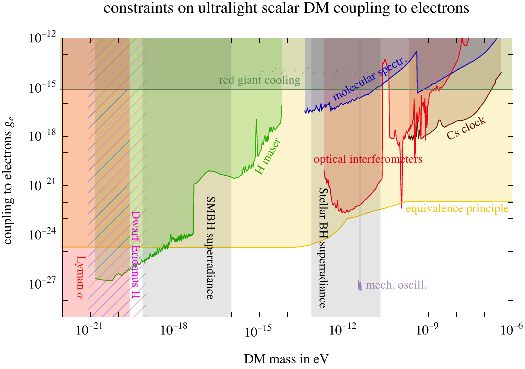
\includegraphics[width=0.72 \textwidth]{figs/plotLSelec}
\end{center}
\caption[Laboratory constraints on light and ultralight scalar DM]{\em\label{fig:SLelec:bounds} 
Laboratory {\bfseries constraints on light and ultralight scalar DM}, assumed to couple only to electrons ($g_e\ne0$  in eq.~\eqref{eq:Leff:phi:UDM}): 
from comparisons of H masers and cavities, molecular spectroscopy of I${}_2$,  optical interferometers, comparison of atomic Cs clock with reference cavity oscillator, and from tests of the equivalence principle \cite{ultra:light:DM:electrons}. There are also bounds from astrophysics (excluded vertical bands, see fig.~\ref{fig:ULDM} and section~\ref{sec:UDM:indirect} for further details),  as well as constraints from the absence of anomalously large cooling rates in red giants, which exclude the upper region of the shown range in $g_e$. 
}
\end{figure}


\item[$\diamond$]
{\bf Torsional balances}  are used to search for non-gravitational forces between macroscopic test masses, by searching for small differential accelerations perpendicular to the torsion fiber.
The light DM as a force carrier can be searched for either in the static limit, where Earth is used as a (large) source of DM induced potential, or in a time-dependent search, where one searches for oscillatory behaviour due to the new DM induced forces \cite{1512.06165}. Such tests also go under the name of {\em 5-th force searches} or {\em tests of the equivalence principle}. 


\item[$\diamond$]
{\bf Axion detectors}. 
Section~\ref{axion} will show that the axion $a$ is a motivated light boson DM candidate that couples
to photons via the $ aF_{\mu\nu}\tilde F^{\mu\nu}= - 4 a \vec E \cdot \vec B$ effective operator. 
In the presence of an external magnetic field $\vec B$, the oscillating DM axion field acts as a new source of electric and magnetic fields, 
which can be used to construct a variety of possible detection techniques, such as 
shining-through wall-experiments, helioscopes and haloscopes, to be discussed in section~\ref{AxionExp}. 
Many of these experiments can be used  to also search for dark photons. 
Since the dark photons interact with SM through kinetic mixing, the signals are then present also in the absence of an external magnetic field, and can be searched for even more readily than the axions. 
A review of uses of axion detectors for dark photon searches can be found in \cite{ultra:light:DM}.

\item[$\diamond$]
{\bf Spin-based sensors}. Axions might also couple to SM fermions via the relativistic operator 
$\partial_\mu a (\bar f_i \gamma^\mu \gamma_5 f_i)/f_{a,i}$, that results in the non-relativistic Hamiltonian
\beq
{\cal H}=-\frac{2}{f_{a,i}}\vec S_i \cdot \vec \nabla a(\vec r, t).
\eeq 
The derivative coupling is a consequence of axion being a result of a spontaneously broken global symmetry (a (pseudo)Nambu-Goldstone boson), while the coupling to nuclear or electron spin, $\vec S_i$, is possible due to the fact that axion is a pseudoscalar.  Vector DM would instead couple as ${\cal H}\propto \vec \phi \cdot \vec S_i$, without derivatives.
Such interactions with DM would therefore appear as a new magnetic-like force acting on nuclear or electron spins, 
and can be searched for using spin-based quantum sensors \cite{2106.09210,axion:nEDM:oscill}, see also section~\ref{AxionExp}.


\item[$\diamond$]
 {\bf Neutrinos}. If DM $\phi$ has an effective Yukawa coupling, 
$\Lag \supset g_\nu \,\phi \nu_L^2/2 + \hbox{h.c.}$, to SM neutrinos,
their masses receive corrections $\delta m_\nu \approx g_\nu \phi  \approx g_\nu \eV  ({\rm meV}/M)$, where the numerical estimate assumes the local DM density and eq.\eq{phi0rho}. 
For light enough DM and big enough $g_\nu$
this coukd lead to a correction comparable or larger than the observed neutrino masses~\cite{DMnumass}. 
However, significant effects from such couplings in present day neutrino experiments are disfavoured by cosmology:
since the DM density was higher in the earlier universe, CMB and BBN observations imply constraints
$g_\nu \lesssim M/\eV$.
Effects in neutrino oscillations compatible with the observed cosmology are possible, 
if DM instead couples to relatively light right-handed neutrinos~\cite{DMnumass}.


\end{itemize}
Fig.~\ref{fig:SLelec:bounds} shows an example of laboratory constraints on the electrophilic light/ultra-light scalar DM (only $g_e$ taken to be nonzero). The bounds from comparisons of Cs clocks and H masers with other resonators  (cavities), are typically less sensitive than the searches for violations of equivalence principle, which test for the presence of a new force mediated by a light scalar. 
See also fig.~\ref{fig:ULDM} and section~\ref{sec:UDM:indirect} for the discussion of astrophysical bounds, and~\cite{ultra:light:DM} for a more detailed discussion of constraints. Another example of a light scalar is the light Higgs-mixed scalar with constraints shown in fig.~\ref{fig:Higgs:mixed:scalar}. Yet another example of a light boson is an axion, with the constraints on axion couplings to photons shown in fig.~\ref{fig:axion}.
 


